\chapter{GeoPaxos with B+ Tree}\label{sec:geopaxos-with-b+tree}
Now that we have discussed the needed background, we can move onto the next step: using a B+ Tree on top of GeoPaxos to store the data objects. A b+tree has many interesting characteristics that make it particularly suitable for some types of applications, but it also brings some new challenges to the table. The data structure has to be indentical in every replica: this means that all the operations done on the tree have to be deterministic and executed in the right order. While this is not particularly complicated on other data structures, such as a HashMap, this becomes more complicated with a tree, where we have many branches and nodes that may split and cause further modifications up to the root.

Furthermore, the usage of GeoPaxos and a tree brings the need for a new type of operation. In GeoPaxos the objects are assigned to one or more groups, or partitions, depending on the type, number and origin of accesses. Of these groups, one will also be chosen in each replica to be the preferred partition for the operation, usually based on geographic location. There has to be a moment when these groups are decided and calculated for each object in the B+ Tree. For this, we have a command called repartition. The command takes the workload of an object, which is the number of reads and writes from each group on this object, and a graph that represents the geographic location of the various replicas. It then calculates the optimal placement of the object in the groups, that with the given workload would give us the minimum average latency.

This operation can take be a big performance bottleneck, since it has to be executed for every object in the tree, and since we have to consider every combination of groups it scales exponentially with the number of groups. We therefore want to find a fast way to perform this operation so that we still get the right assignment of objects in a short amount of time.

In the following sections of this chapter we will first explain what a B+ Tree is, how it works and what are its advantages and disadvantages. We will then describe the specific B+ Tree used in our application. Then we will go over the various approaches that were attempted to improve the performance of the repartition optimization, followed with tests on the performance of the repartition operation only and finally with GeoPaxos as well.

\section{B+ Tree}\label{sec:b+tree}
The B+ Tree is the data structure that was chosen to store the data in the geo-replicated servers. Since the B+ Tree is a special case of a B-Tree, let us quickly mention what a B-Tree is.

A B-Tree is a self-balancing data structure; it is a more general version of a binary search tree, since it allows nodes to have an arbitrary number of children, instead of two like in a binary search tree. Its advantage is that one node can have an increased number of children (this number being called the \emph{branching factor}), making it more efficient to retrieve large amounts of data at once. Also, its time complexities for search, insertion and deletion are still $O(log n)$.

A B+ Tree is similar to a B-Tree, but all its data items are stored at the leaves of the tree. It has three types of nodes: the root node, the inner nodes and the leaves. The leaves are the nodes at the lowest level of the tree, which we call level 0, that can only point to data items; inner nodes can be found from levels higher than 0, and they can point to other inner nodes or to leaf nodes. The root is a special case, as it is initially a leaf node when the tree is empty, but when the tree starts to fill up it will act as an inner node. Also, the branching factor of a B+ Tree can be quite high, particularly compared to a B-Tree. In our implementation, for example, we use a branching factor of $b=100$.

The main advantage of the B+ Tree, similarly to a B-Tree, is still when it comes to accessing big amounts of data at once. Say, for example, that we want to perform some operation on a range of elments. Since the data items are all at the leaves and grouped together, we can retrieve at once hundreds of data items with few operations.

Give a branching factor of $b$, leaf nodes and inner nodes can have a number of children between $\lceil b/2 \rceil$ and $b$. this means that in our implementation, with $b=100$, leaf nodes and inner nodes will always have between 50 and 100 children. The exception is the root, which initially will have only one children, and it will act as a leaf. Once it reaches $b-1$ data items, two inner nodes are created, they become children of the root and they get half of the data items each; at this point, the root will start acting like an inner node, with a minimum of 2 children up to $b$.

The splitting of nodes is similar to other self-balancing trees: when a node reaches the maximum number of children allowed by the maximum branching factor, a new node is created, and half of the children of the full node are given to the new node. Since then the new node has to be appended to the parent's children, a split may propagate up to the root of the tree.

\begin{figure}[!htb]
    \centering
    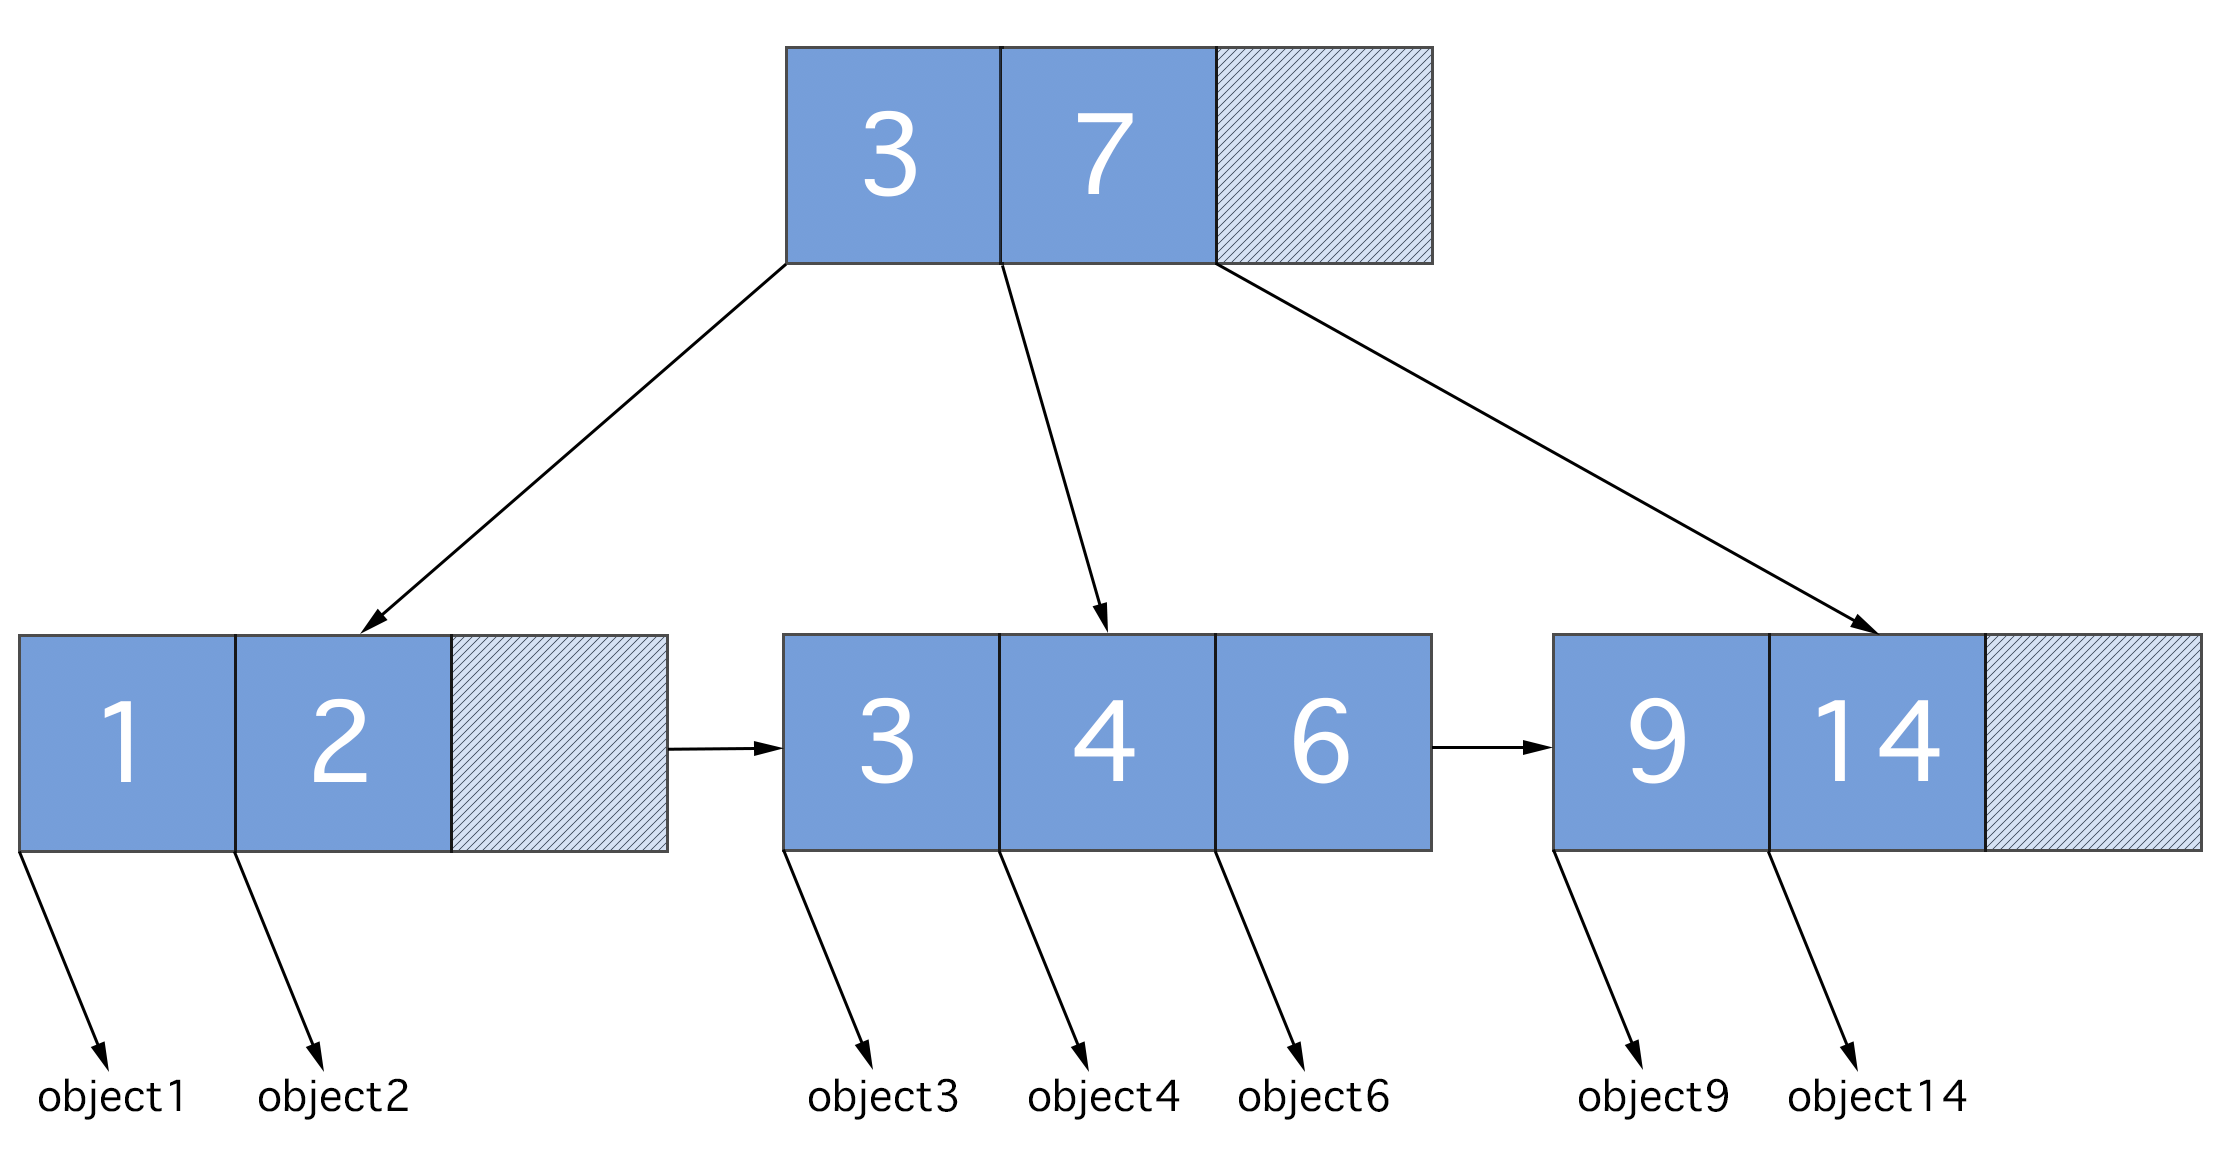
\includegraphics[width=\textwidth,height=\textheight,keepaspectratio]{img/b+tree.png}
    \caption{ An example of B+ Tree with a branching factor of $b=4$. We have a root node that acts as an inner node, meaning that its children are nodes themselves. The children nodes are leaf nodes, with their children being the actual objects that are being stored. }
    \label{fig:b+tree}
\end{figure}

% [add characteristics from wiki?]

\subsection{B+ Tree Implementation}\label{sec:b+tree-implementation}
For our application, the basic B+ Tree needs to have some extra characteristics added to it. 

First of all, each node (root, inner and leaf nodes) will store statistics based on the operations performed. In particular, each node will have two counters, one for read and one for write operations, for each group in the system. Therefore, if we have three groups, each node will have six counters. The statistics are updated from the root up to the node that handles the item accessed. 

\begin{figure}[!htb]
  \centering
  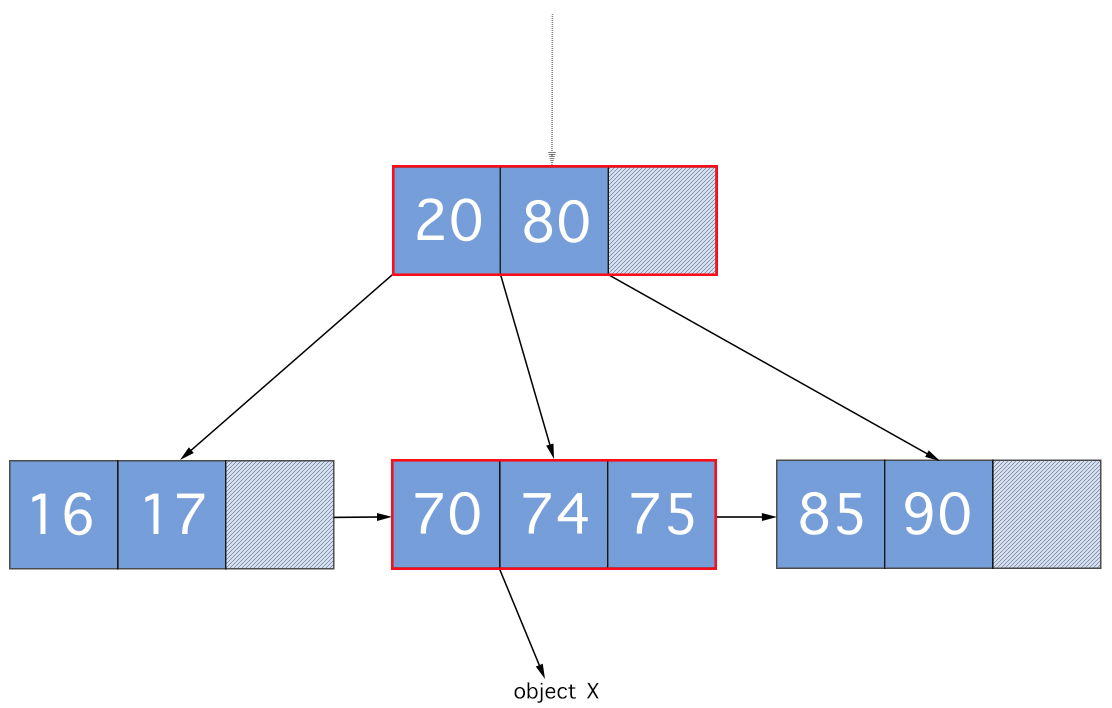
\includegraphics[width=\textwidth,height=\textheight,keepaspectratio]{img/b+tree_path.png}
  \caption{ When an operation on \emph{some object} is performed, we update the statistics on all the nodes on the path to the object. In this example, if we perform a read on said object, we increase the reads counter on both the red nodes.}
  \label{fig:b+tree_path}
\end{figure}

These statistics will be used as \emph{workload} when the repartition will be issued. Once the repartition is performed, the statistics will be updated with the formula:
$$ current\_statistics = \alpha \cdot old\_statistics + (1-\alpha) \cdot new\_statistics $$
Where the old statistics are the ones gathered until the past repartition, and the new statistics are the ones between the past repartition and the current one (See Figure \ref{fig:statistics}).
Alpha is the aging factor, which determines how much importance we give to the old and new statistics. a small alpha gives more weight to recent ones, but it also makes the system more susceptible to unexpected variations in the workloads.

\begin{figure}[!htb]
  \centering
  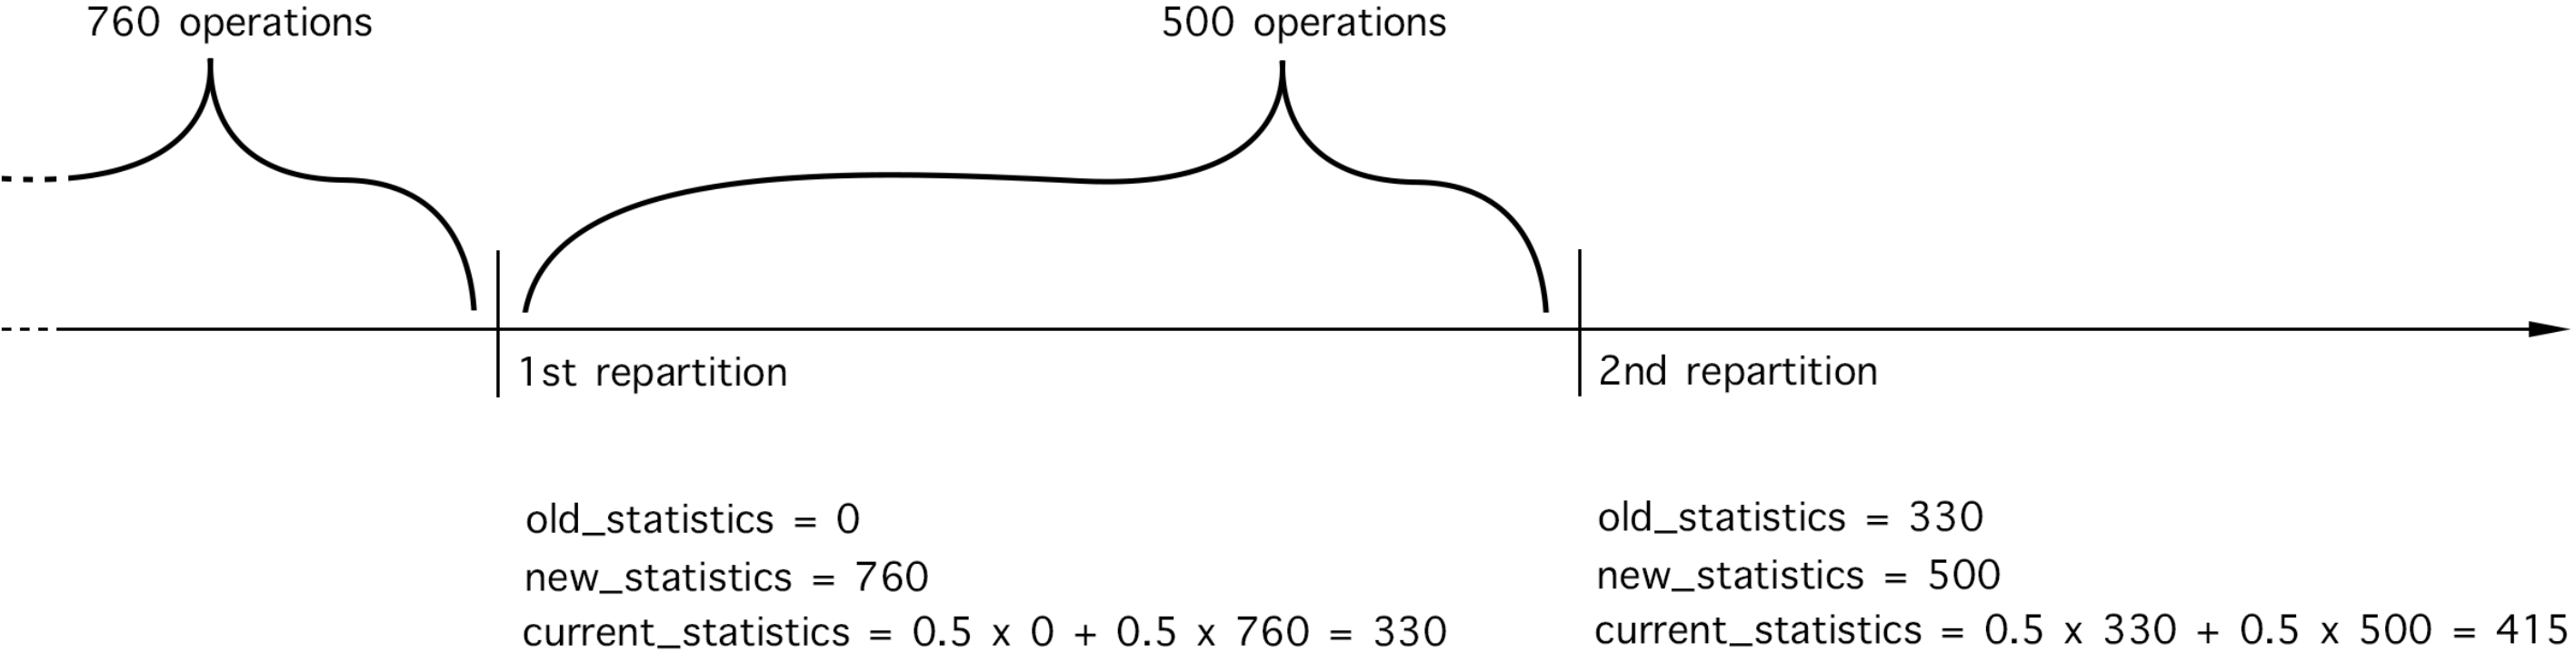
\includegraphics[width=\textwidth,height=\textheight,keepaspectratio]{img/statistics.png}
  \caption{An example of how the statistics are updated for each node after every repartition, with $alpha = 0.5$. Before the first repartition we have 760 operations on the objects handled by this node. When the first repartition is issued, we calculate the current statistics using the old and new statistics. For the second repartition, the previous current statistics will become the old statistics, and the new statistics will be the ones performed between the first and second repartition. }
  \label{fig:statistics}
\end{figure}

Furthermore, whenever a node is full and it has to split, its statistics are halved evenly between the two nodes. This is because we do not know which statistics correspond to which data item in particular, but we can assume that there is a decent chance that objects that are close to each others will have similar statistics, meaning that we expect them to have good locality.

The second thing that we need to store in the nodes of our B+ Tree are the partitions. In particular, we need to store both the \emph{partitions} that take care of each node and the \emph{preferred partition} in case there are multiple partitions to choose from. Initially, each new node will be assigned to all partitions of the system. This is to make sure that all clients will initially have the same availability of the data items. Once we issue a repartition, the algorithm will calculate the optimal partitions for each node based on the workload. These optimal repartition will be used to know which replicas to involve in the subsequent operations on each object, until the next repartition.

If a node splits, the new node will inherit the partitions from the full node. This is again a heuristic, based on the high likelihood that close objects will have similar accesses.

\subsection{System Implementation}\label{sec:system-implementation}
The implementation of the B+ Tree data structure, the repartition algorithms and the further code necessary to use this structure on top of GeoPaxos was written in C++. Since this is built on top of the GeoPaxos library, there is also the requirement for the libraries needed by GeoPaxos itself, in particular libevent[link] for the networking part, libpaxos for consensus[link] and libmcast[link] for atomic multicast.

\section{Optimization Approaches}\label{sec:optimization-approaches}
In this section we will first explain in detail how we calculate the optimal group assignment of data objects to the partitions based on the workload. We will then go over the various approaches that were attempted to improve the repartition process. 

\subsection{Optimal Partitions Algorithm}\label{sec:optimal-partitions-algorithm} 
The simplest algorithm to come up with is the one that compares all the possible combinations of partitions and picks the best one. While this algorithm will give the optimal assignments for minimum average latency for a certain workload, it is also the one that takes the largest amount of time. We will use the performance of this algorithm as a benchmark to compare against our later algorithms.

The pseudocode of this algorithm can be found in Algorithm \ref{alg:all-combinations}. This algorithm goes top to bottom and it calculates the partitions for each node. The workload of a node will have a structure similar to the one shown in Table \ref{tab:workload-example}.

\begin{table}[!htb]
  \centering
  \begin{tabular}{l l l l}
    \hline
    & \textbf{Group 1} & \textbf{Group 2} & \textbf{Group 3} \\
    \hline
    \textbf{Reads} & 150 & 37 & 540 \\
    \textbf{Writes} & 32 & 10 & 93 \\
    \hline
  \end{tabular}
  \caption{Example of a possible workload of a node in a case with three groups. The node counts the number of read and write operations received from each group, to be used for the repartition algorithm.}\label{tab:workload-example}
\end{table}

We then load a graph that represents the geographic placements of the various replicas, where the cost of the edges is the estimated average Round Trip Time required to send a message (See Figure \ref{fig:graph}).

\begin{figure}[!htb]
  \centering
  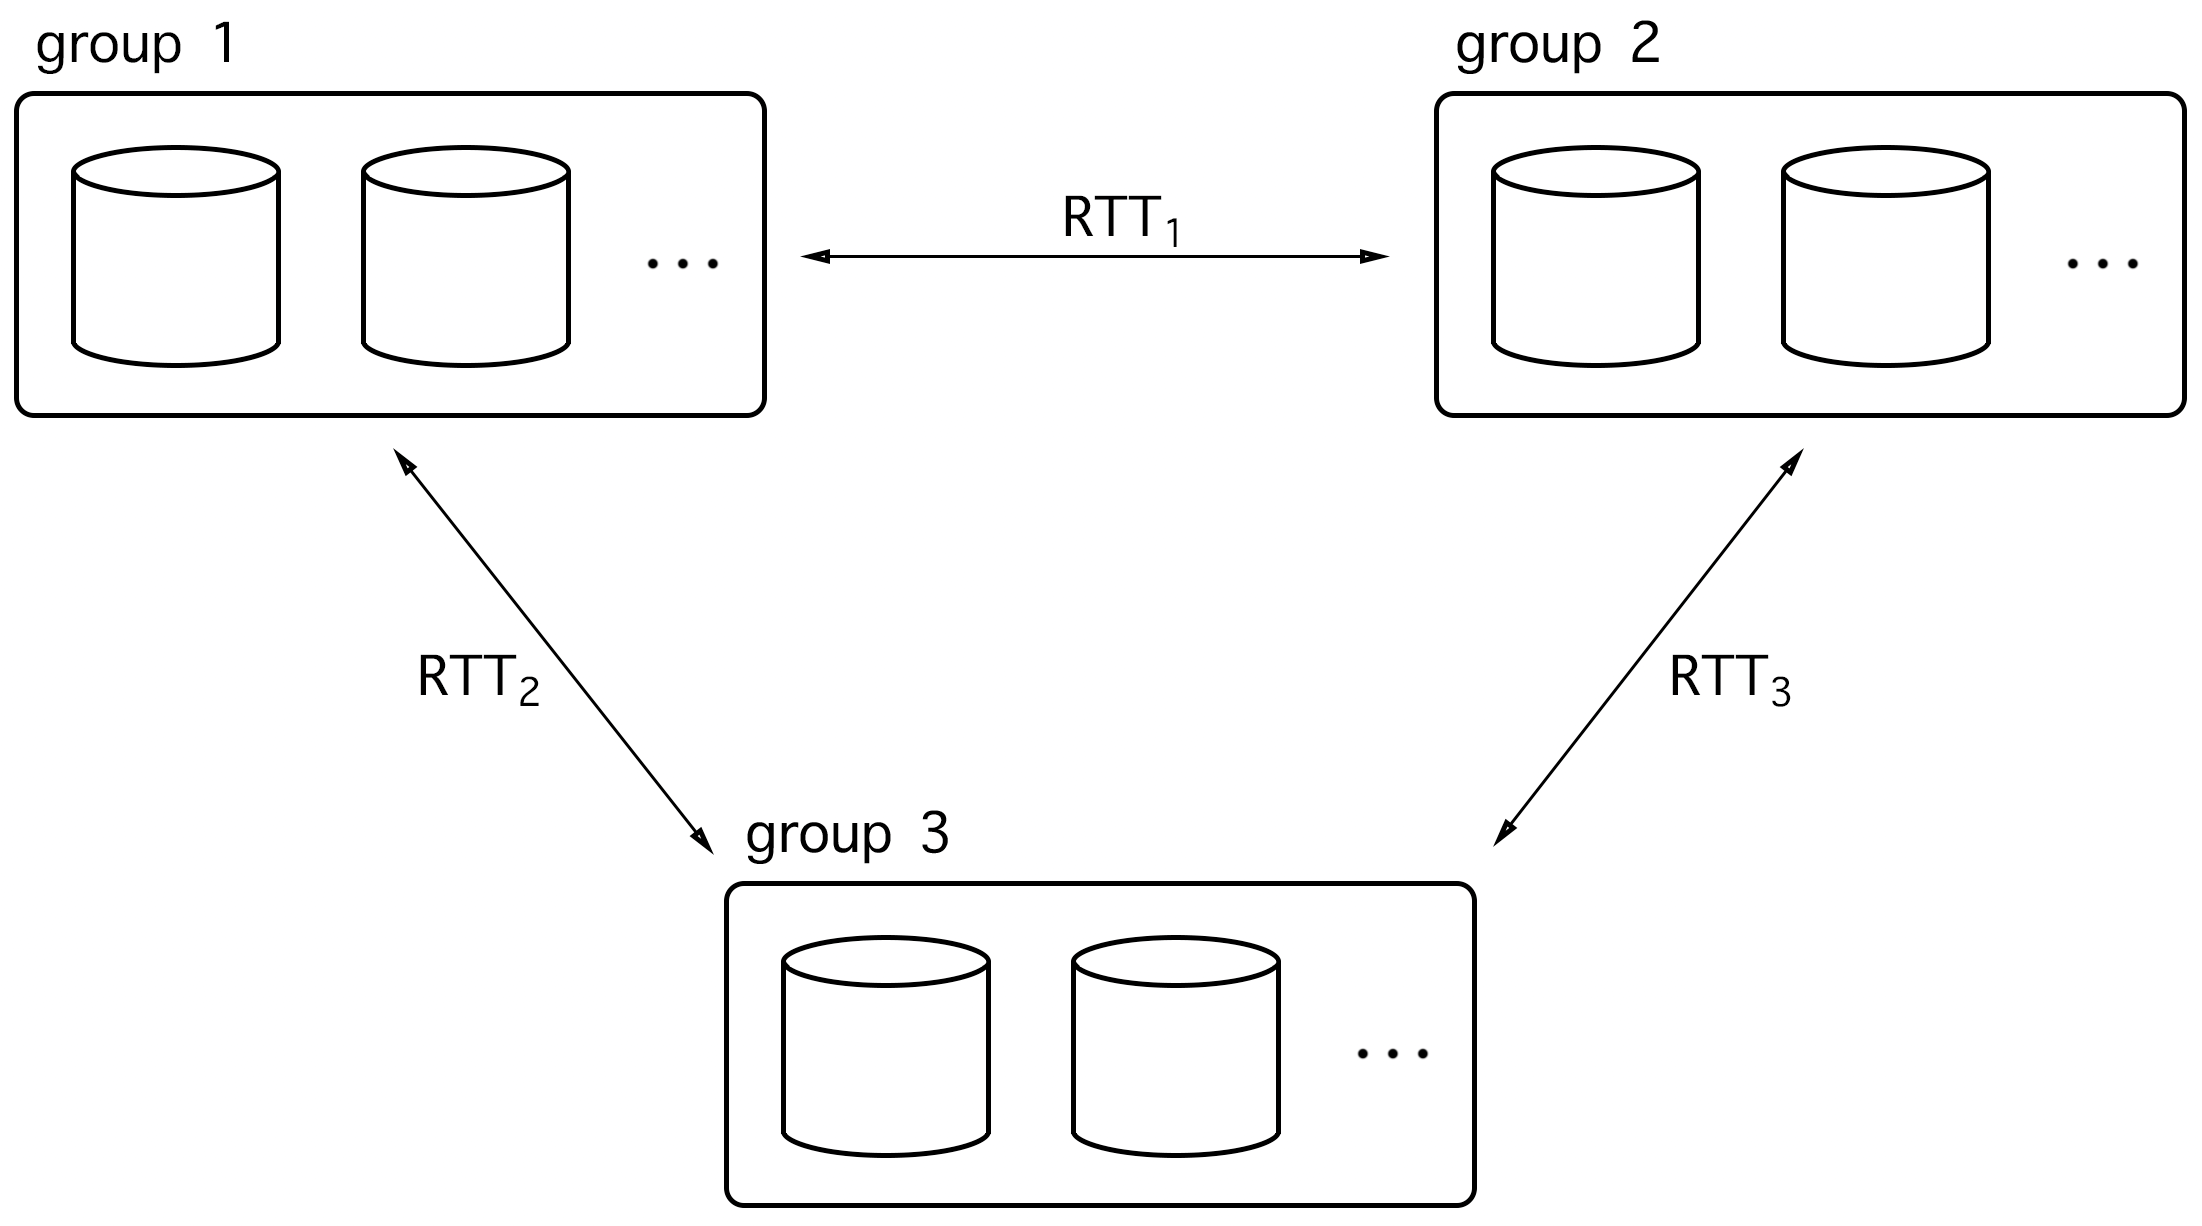
\includegraphics[width=\textwidth,height=\textheight,keepaspectratio]{img/graph.png}
  \caption{An example of a graph representing a geographically distributed environment. Each of the three groups are placed far away, with Round Trip Times defined between each pair of groups. Each group will have multiple replicas in its area, with negligible latency.}
  \label{fig:graph}
\end{figure}

We then proceed by looping over all possible combinations of partitions, where a partition can be either taken or not taken. Logically, at least one partition has to be taken, since we need the object to be assigned to at least one group. In the case of 3 groups, we would have to consider $2^3 -1 = 7$ combinations: $001, 010, 100, 011, 101, 110, 111$, where 1 and 0 mean that the object will be or will not be assigned to that specific replica.

Given the number of reads and writes for each group, and the current groups to which we are replicating this object, we multiply the number of reads by the latency with the closest replica that would have this object. For writes, we have to add the latency of all the replicas that have this object, since the operation is going to modify the data item.

Also note that the result depends on the latency that we are currently considering: for example, if we are doing the calculations from the point of view of a replica that will not have this object, each read will have to go to a different replica; therefore we have to consider the costs from the point of view of all the replicas.

Once we have gone over all the combinations, we pick the one with the lowest cost, and we move onto the next object.

% \begin{algorithm}
%   \caption{All-Combinations}\label{alg:all-combinations}
%   \begin{algorithmic}[1]
%   \Function{repartition}{}:
%   \State $repartition\_tree(root)$
%   \EndFunction
%   \Function{repartition\_tree}{$node$}:
%     \If {$node.has\_changed$}
%       % \State $vw = vector(node.statistics)$
%       \State $topology = new\ topology(node.workloads)$
%       \State $g = topology.calculate\_min\_cost\_graph()$
%       \For {$vertex \in g$}:
%         \If {$vertex.has\_object$}:
%         \State $node.partitions += vertex$
%           \If {$vertex == my\_partition\ \wedge vertex.has\_object$}
%             \State $node.preferred\_partition = vertex$
%           \EndIf
%         \EndIf
%       \EndFor
%     \EndIf
%     \If{$!node\ is\ leafnode$}:
%       \For {$child\ \in\ node.child\_nodes$}:
%         \State $repartiton\_tree(child)$
%         \EndFor
%     \EndIf
%     \EndFunction
%     \Function{calculate\_min\_cost\_graph}{}:
%     \State $min\_cost = \infty$
%       \ForAll {$graph\ combination$}:
%         \State $cost = calculate\_cost(graph, vertices)$
%         \If {$cost < min\_cost$}:
%           \State $min\_cost = cost$
%           \State $min\_graph = graph$
%         \EndIf
%       \EndFor
%     \State \textbf{return} $min\_graph$
%     \EndFunction
%     \Function{calculate\_cost}{$vertex$}:
%       \State $in\_reads, out\_reads, in\_writes, out\_writes = 0$
%       \State $reps = |vertex \in graph.vertices \mid vertex.has\_object|$
%       \For {$vertex \in graph.vertices$}:
%       \State $min\_weight = nearest vertex \in graph | vertex.has\_object$
%       \State $max\_weight = furthest\ vertex \in graph | vertex.has\_object$
%         \If {$vertex.has\_object$}:
%           \State $in\_reads+= 1$
%           \If {$rep\_size > 1$}:
%           \State $\in\_writes+= vertex.writes$
%           \Else
%           \State  $\in\_writes+= 1 $
%           \EndIf
%         \Else:
%           \State $out\_reads += vertex.reads \cdot min\_weight$
%           \State $out\_writes += vertex.writes \cdot min\_weight$
%         \EndIf
%       \EndFor
%       \State $cost = in\_reads+ out\_reads + (in\_writes+ out\_writes) \cdot max\_weight$
%       \State \textbf{return} $cost$
%   \EndFunction
%   \end{algorithmic}
%   \end{algorithm}

\subsection{Fixed-Size Buckets}\label{sec:Fixed-Size buckets}
One of the ideas to improve the performance of the repartition is to try to reduce the number of nodes that we have to do the calculations for.

Since the tree is divided in levels, the idea is to group nodes of different levels in what we call \emph{buckets} and do an aggregated calculation of the optimal partition assignment for the whole bucket. An example of a bucket can be seen in figure ~\ref{fig:Fixed-Size-buckets}. The pseudocode can be found in Algorithm \ref{alg:fixed-size}.

As a reminder, whenever a operation is performend on an object, the statistics of the tree are updated along the whole path from the root to the node that handles this object. This means that in general, the parent node will have the aggregated statistics for all its children nodes (this may not always be the exact case when the parent node splits, but this is quite rare, and even when it happens the statistics of the split nodes are good approximations of the real statistics).

There are also multiple ways to group nodes in the case where we have an odd number of levels. Since we are using buckets of two levels, we could either allow the root node to be a bucket of 1 level, or let the leaves be buckets of 1 level. Or, we could have the root be the only bucket to be allowed to have 3 levels. The first one would not reduce the number of saved calculations by much, since most nodes are on level 0; the other two options make virtually no difference, as they only affect the level with the least amount of nodes. We decided to go with the second option, allowing the root node to be in a bucket of its own in case of an odd number of levels.

It is also important to remember that this improvement affects only the number of objects, not the groups; therefore, in the case where we have $n$ objects and $m$ groups, this would improve on the linear number of objects $n$ but it would not affect the number of combinations, which grows as $2^m$.

In general, given a branching factor of $b$ of and objects $n$, the number of calculations we would be doing would be around $\approx\cfrac{n}{b}$ as the tree grows, since we are approximating all the calculations at level 0, which is by far the level with the most nodes.

This approach will generally work best in cases where we have a great amount of locality, meaning that the heuristic of grouping nodes together expecting them to have similar behavior would be mostly correct. Even in that case, though, we expect to still see repartitioning results that are not optimal.

[should I be more precise with the number of calculations saved?]

\begin{figure}[!htb]
  \centering
  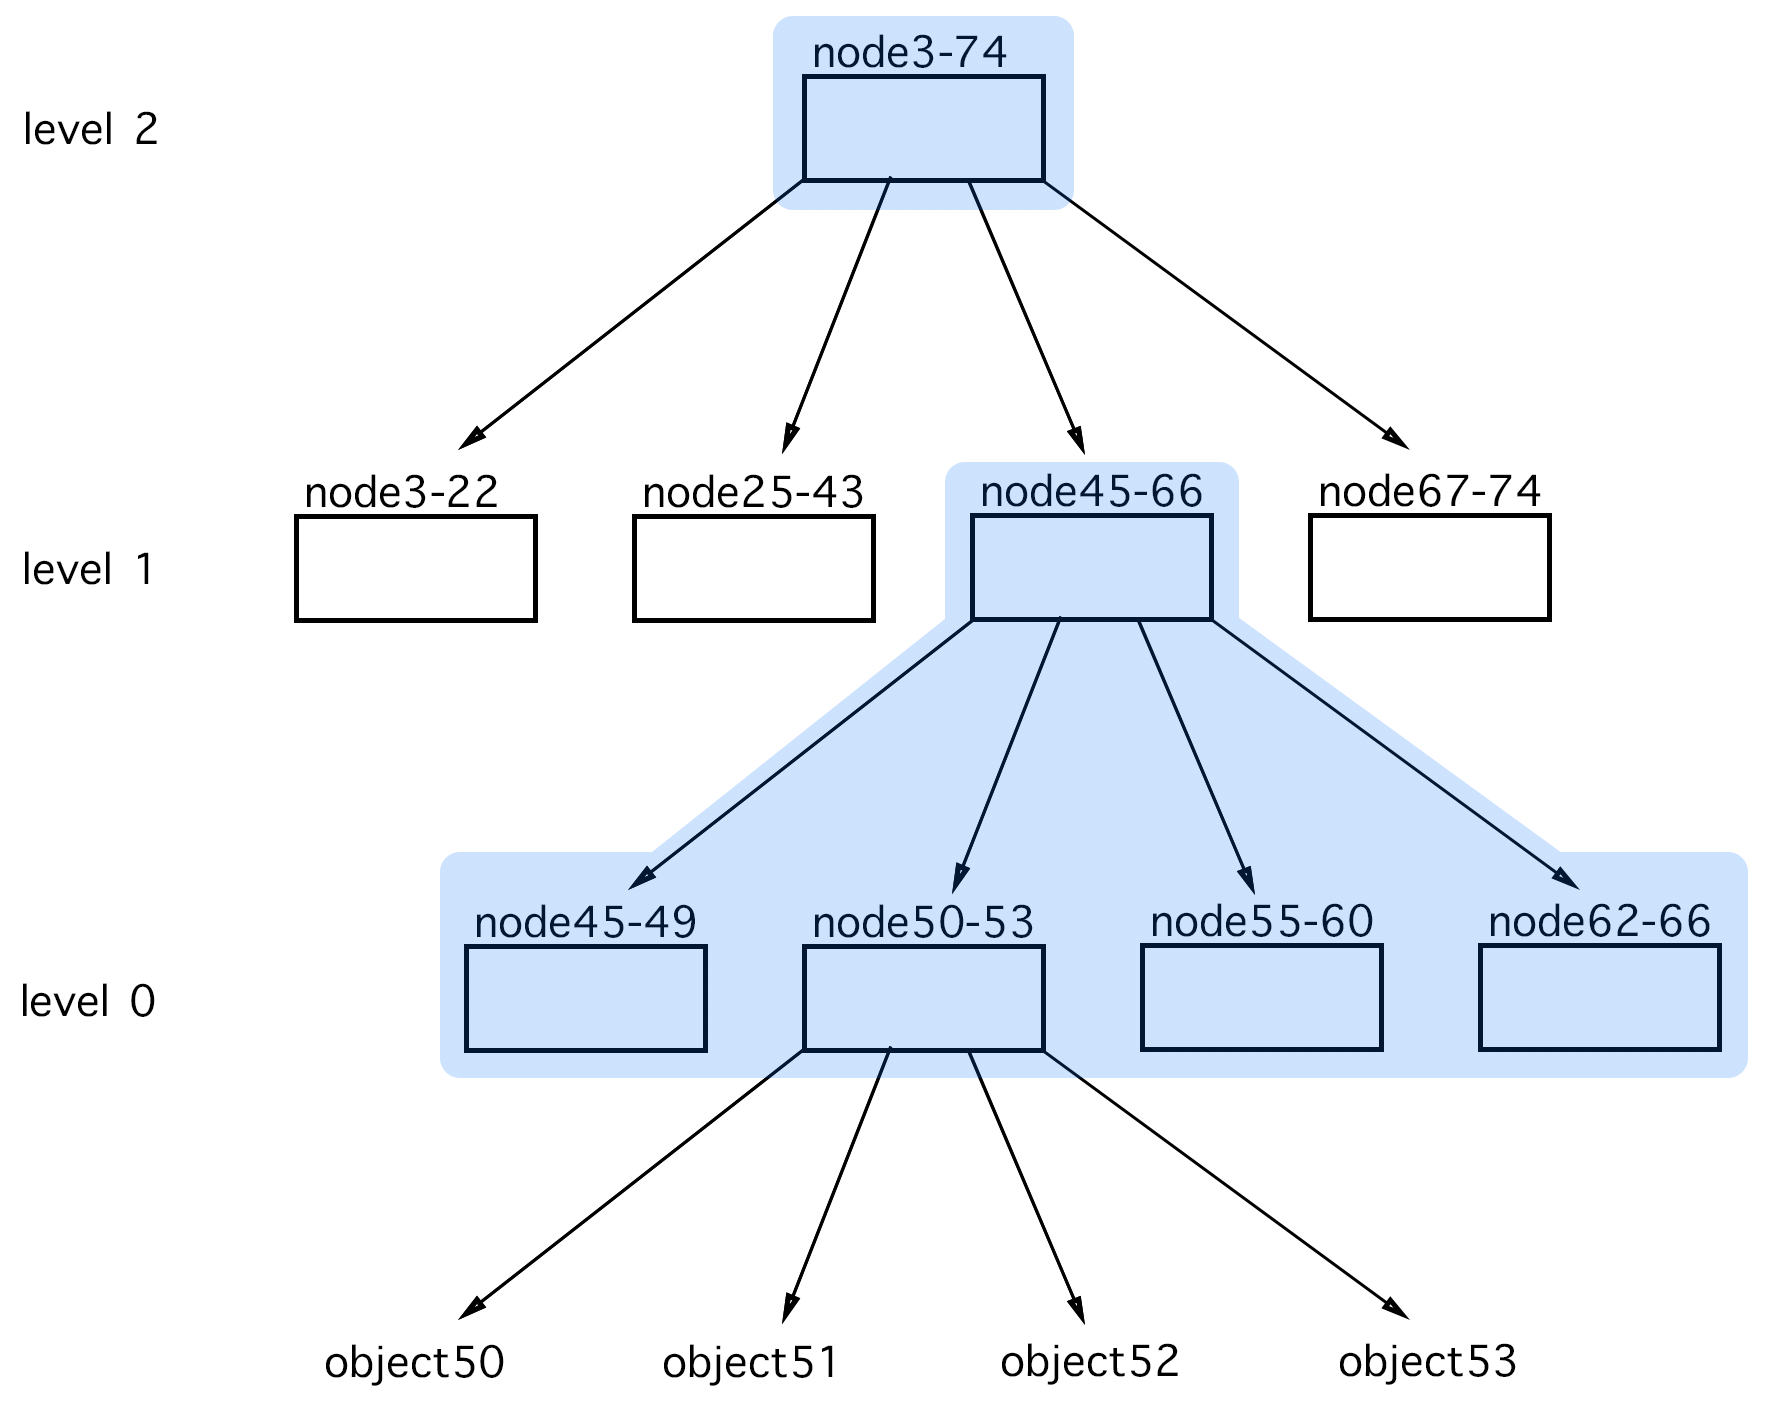
\includegraphics[width=\textwidth,height=\textheight,keepaspectratio]{img/grouped-levels.png}
  \caption{ A visualization of how the levels are grouped. The nodes in the same triangles are going to have the same partitioning, based on the aggregated statistics (which are going to be the statistics of the highest-level node). The root at level 2 is in its own bucket, since we have an odd number of levels. Also note that only a few nodes are shown too keep the visualization simple.}
  \label{fig:Fixed-Size-buckets}
\end{figure}

% \begin{algorithm}
%   \caption{Fixed-Size Buckets}\label{alg:fixed-size}
%   \begin{algorithmic}[1]
%     \Function{repartition}{}:
%   \State $repartition\_tree(root, true)$
%   \EndFunction
%   \Function{repartition\_tree}{$node, is\_root$}:
%   \State $is\_bucket\_root = node.level\ is\ odd \vee is\_root$
%     \If {$node.has\_changed \vee is\_bucket\_root$}:
%       % \State $vw = vector(node.statistics)$
%       \State $topology = new\ topology(node.workloads)$
%       \State $g = topology.calculate\_min\_cost\_graph()$
%       \For {$vertex \in g$}:
%         \If {$vertex.has\_object$}:
%         \State $node.partitions += vertex$
%           \If {$vertex == my\_partition\ \wedge vertex.has\_object$}
%             \State $node.preferred\_partition = vertex$
%           \EndIf
%         \EndIf
%       \EndFor
%     \EndIf
%     \If{$!node\ is\ leafnode$}:
%       \For {$child\ \in\ node.child\_nodes$}:
%       \If {$is\_bucket\_root = node.level\ is\ odd$}:
%         \State $child.partitions = node.partitions$
%         \State $child.preferred\_partition = node.preferred\_partition$
%       \EndIf
%         \State $repartiton\_tree(child, false)$
%         \EndFor
%     \EndIf
%     \EndFunction
%     \Function{calculate\_min\_cost\_graph}{}:
%     \State $min\_cost = \infty$
%       \ForAll {$graph\ combination$}:
%         \State $cost = calculate\_cost(graph, vertices)$
%         \If {$cost < min\_cost$}:
%           \State $min\_cost = cost$
%           \State $min\_graph = graph$
%         \EndIf
%       \EndFor
%     \State \textbf{return} $min\_graph$
%     \EndFunction
%     \Function{calculate\_cost}{$vertex$}:
%       \State $in\_reads, out\_reads, in\_writes, out\_writes = 0$
%       \State $reps = |vertex \in graph.vertices \mid vertex.has\_object|$
%       \For {$vertex \in graph.vertices$}:
%       \State $min\_weight = nearest\ vertex \in graph | vertex.has\_object$
%       \State $max\_weight = furthest\ vertex \in graph | vertex.has\_object$
%         \If {$vertex.has\_object$}:
%           \State $in\_reads+= 1$
%           \If {$rep\_size > 1$}:
%           \State $\in\_writes+= vertex.writes$
%           \Else
%           \State  $\in\_writes+= 1 $
%           \EndIf
%         \Else:
%           \State $out\_reads += vertex.reads \cdot min\_weight$
%           \State $out\_writes += vertex.writes \cdot min\_weight$
%         \EndIf
%       \EndFor
%       \State $cost = in\_reads+ out\_reads + (in\_writes+ out\_writes) \cdot max\_weight$
%       \State \textbf{return} $cost$
%   \EndFunction
%   \end{algorithmic}
%   \end{algorithm}

\subsection{Variable-Size Buckets}\label{sec:Variable-Size buckets}
The idea of the Fixed-Size buckets is interesting, as it greatly reduces the number of nodes we have to account for, but it also generalizes the situation, grouping the nodes regardless of their workload. Reducing the branching factor would not be a solution, as it would just increase the number of nodes once again, and because the high branching factor is one of the main reasons to use a B+ Tree. 

An alternative approach is to to have a variable, or dynamic, size of buckets. The idea is to group in two or more levels the nodes that have a low amount of statistics, and instead do the optimal calculations for the nodes with many operations associated to them. The idea is that approximating the nodes with few operations would not hinder the performance by much, as the object associated to those nodes will not be accessed often by the clients, while instead the objects that are accessed often will have their optimal partitions. 
The pseudocode for this method is in Algorithm \ref{alg:variable-size}.


One challenge of the Variable-Size buckets approach is to figure out when it is worth doing the full calculations and when it is better to group in buckets. In the case where the operations are evenly distributed among all children of a node, we would expect have that the statistics of a child node will be around $\cfrac{1}{b}$ of the parent node. Then, we could say that if, for example, a child node has less than $\cfrac{1}{b^2}$, then we should place it in a bucket; but finding the right number depends on many variables and on the system at hand, therefore finding a good value would have to be fine-tuned depending on the application.

\begin{figure}[!htb]
  \centering
  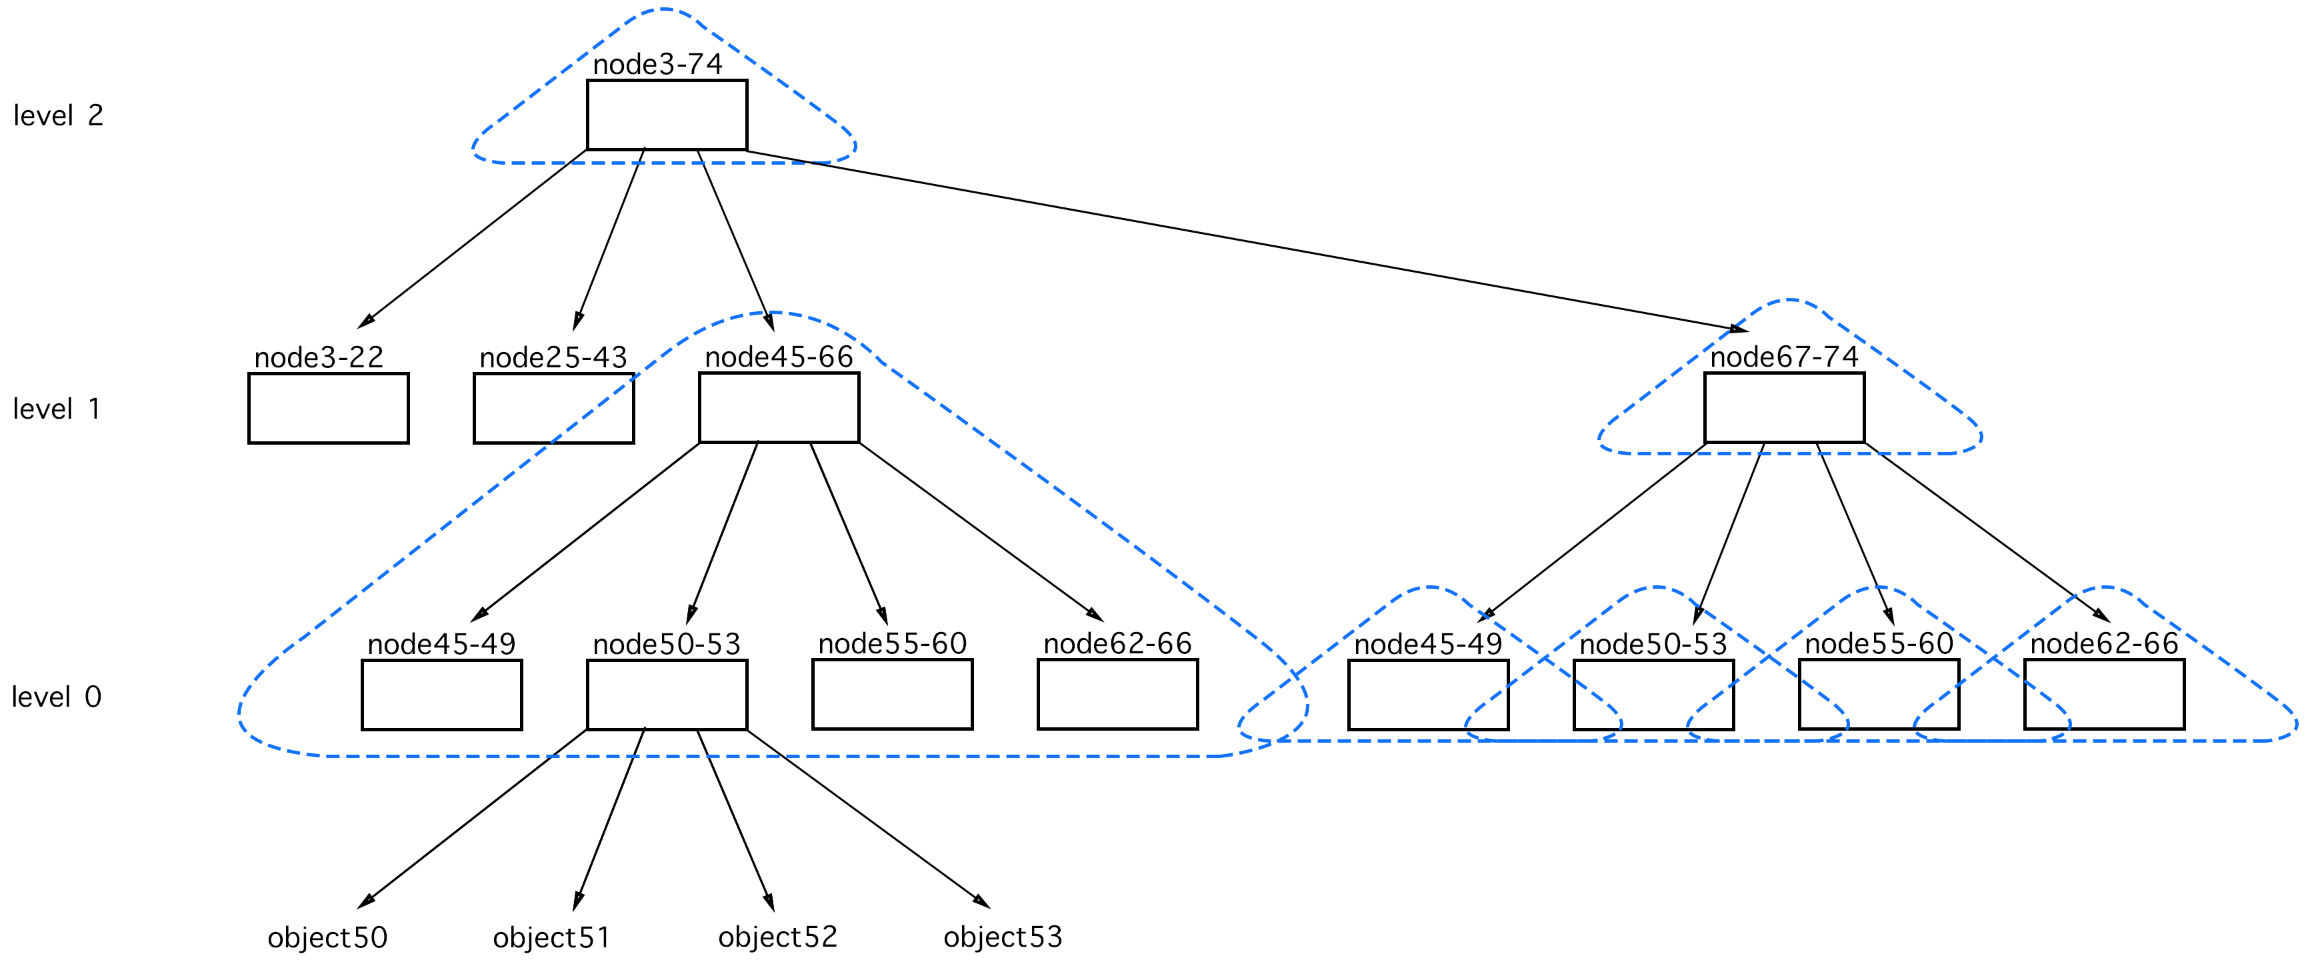
\includegraphics[width=\textwidth,height=\textheight,keepaspectratio]{img/dynamic-buckets.png}
  \caption{ A visualization of a variable-size grouping. Node 45-66 has few operations, therefore it will group all its children into one bucket. Node 67-74 instead has more operations, therefore performing a better partitioning might give us better improvements; therefore, this node will not group its children, and we will calculate the optimal partition for those nodes. }
  \label{fig:Variable-Size-buckets}
\end{figure}

% \begin{algorithm}
%   \caption{Variable-Size Buckets}\label{alg:variable-size}
%   \begin{algorithmic}[1]
%     \Function{repartition}{}:
%   \State $repartition\_tree(parent\_node, workload\_ratio)$
%   \EndFunction
%   \Function{repartition\_tree}{$node, is\_root$}:
%     \State $my\_workload = 0$
%     \If {$node.has\_changed$}:
%       \State $my\_workload = sum(node.workloads)$
%       \If {$my\_workload < workload\_ratio * treshold$}:
%       \State $child.partitions = parent.partitions$
%       \State $child.preferred\_partition = parent.preferred\_partition$
%       \Else
%       \State $topology = new\ topology(node.workloads)$
%       \State $g = topology.calculate\_min\_cost\_graph()$
%       \For {$vertex \in g$}:
%         \If {$vertex.has\_object$}:
%         \State $node.partitions += vertex$
%           \If {$vertex == my\_partition\ \wedge vertex.has\_object$}
%             \State $node.preferred\_partition = vertex$
%           \EndIf
%         \EndIf
%       \EndFor
%     \EndIf
%     \EndIf
%     \If{$!node\ is\ leafnode$}:
%       \For {$child\ \in\ node.child\_nodes$}:
%         \State $repartiton\_tree(child, false)$
%         \EndFor
%     \EndIf
%     \EndFunction
%     \Function{calculate\_min\_cost\_graph}{}:
%     \State $min\_cost = \infty$
%       \ForAll {$graph\ combination$}:
%         \State $cost = calculate\_cost(graph, vertices)$
%         \If {$cost < min\_cost$}:
%           \State $min\_cost = cost$
%           \State $min\_graph = graph$
%         \EndIf
%       \EndFor
%     \State \textbf{return} $min\_graph$
%     \EndFunction
%     \Function{calculate\_cost}{$vertex$}:
%       \State $in\_reads, out\_reads, in\_writes, out\_writes = 0$
%       \State $reps = |vertex \in graph.vertices \mid vertex.has\_object|$
%       \For {$vertex \in graph.vertices$}:
%       \State $min\_weight = nearest\ vertex \in graph | vertex.has\_object$
%       \State $max\_weight = furthest\ vertex \in graph | vertex.has\_object$
%         \If {$vertex.has\_object$}:
%           \State $in\_reads+= 1$
%           \If {$rep\_size > 1$}:
%           \State $\in\_writes+= vertex.writes$
%           \Else
%           \State  $\in\_writes+= 1 $
%           \EndIf
%         \Else:
%           \State $out\_reads += vertex.reads \cdot min\_weight$
%           \State $out\_writes += vertex.writes \cdot min\_weight$
%         \EndIf
%       \EndFor
%       \State $cost = in\_reads+ out\_reads + (in\_writes+ out\_writes) \cdot max\_weight$
%       \State \textbf{return} $cost$
%   \EndFunction
%   \end{algorithmic}
%   \end{algorithm}

\subsection{Hot Groups}\label{sec:hot-groups}
Another option is to try to reduce the number of combinations that we have to consider for each node. Since the complexity grows exponentially with the number of groups, if we are able to discard some combinations before we calculated their actual cost, then we should have a greater improvement compared to the optimizations that reduce the number of nodes.

One idea to do this is as follows: given a workload, there is a chance that one or more groups will have fewer operations on the current node compared to other groups. Then, there is a big chance that the final partition assignment would not assign the objects to the group with fewer operations, since the gain of replicating the object to said partition would be less than the added cost of it.

The cost of replicating to a group with few operations also depends on the ratio between read and write operations: with many reads we would want to assign the object to all groups, while with many writes we would want to reduce the number of group assignments for each object, as with every write we would have to coordinate between all groups involved. In general, though, such a system is better suited for applications with more reads than writes, therefore our assumption of discarding groups with few operations still holds.

The way to implement this is fairly simple: with the workload at hand, we find the group or groups with the highest number of operations (the \emph{Hot Groups}). Then, when we are going through all the possible combinations of groups, we discard those that would assign the object to groups with much lower operations than the Hot Groups.  See Algorithm \ref{alg:fixed-size} for the pseudocode.

As before, finding the ideal threshold is not an easy task; a higher threshold would discard more combinations, making the computations faster but possibly lose a lot of accuracy, while a lower threshold might only skip very few combinations giving us very small performance improvements. 


\begin{table}[!htb]
  \centering
  \begin{tabular}{l l l l}
    \hline
    & \textbf{Group 1} & \textbf{Group 2} & \textbf{Group 3} \\
    \hline
    \textbf{Reads} & 150 & 37 & 540 \\
    \textbf{Writes} & 32 & 10 & 93 \\
    \hline
  \end{tabular}

  \caption{Example of a possible workload of a node in a case with 3 groups. In this case, group 3 would be the hot group, since it is the node with more total operations. Depending on the threshold, we could discard only group 2 or both group 1 and 2 from the list of possible assignment combinations; this would reduce the number of combinations for this node from 7 to 3 or 1, respectively.}\label{tab:hot-groups-example}
\end{table}

% \begin{algorithm}
%   \caption{Hot Groups}\label{alg:hot-groups}
%   \begin{algorithmic}[1]
%   \Function{repartition}{}:
%   \State $repartition\_tree(root)$
%   \EndFunction
%   \Function{repartition\_tree}{$node$}:
%     \If {$node.has\_changed$}
%       % \State $vw = vector(node.statistics)$
%       \State $topology = new\ topology(node.workloads)$
%       \State $g = topology.calculate\_min\_cost\_graph()$
%       \For {$vertex \in g$}:
%         \If {$vertex.has\_object$}:
%         \State $node.partitions += vertex$
%           \If {$vertex == my\_partition\ \wedge vertex.has\_object$}
%             \State $node.preferred\_partition = vertex$
%           \EndIf
%         \EndIf
%       \EndFor
%     \EndIf
%     \If{$!node\ is\ leafnode$}:
%       \For {$child\ \in\ node.child\_nodes$}:
%         \State $repartiton\_tree(child)$
%         \EndFor
%     \EndIf
%     \EndFunction
%     \Function{calculate\_min\_cost\_graph}{}:
%     \State $min\_cost = \infty$
%     \State $max\_rw = 0$
%     \For $vertex \in graph$:
%       \If {$vertex.read + vertex.write > max\_rw$}:
%         \State $max\_rw = vertex.read + vertex.write$
%       \EndIf
%     \EndFor
%     \ForAll {$graph\ combination$}:
%       \For {$vertex \in combination$}:
%         \If {$(vertex.reads + vertex.writes) / max\_rw < threshold:$}
%           \State $skip\ combination$
%         \EndIf
%       \EndFor
%       \State $cost = calculate\_cost(graph, vertices)$
%       \If {$cost < min\_cost$}:
%         \State $min\_cost = cost$
%         \State $min\_graph = graph$
%       \EndIf
%     \EndFor
%     \State \textbf{return} $min\_graph$
%     \EndFunction

%     \Function{calculate\_cost}{$vertex$}:
%       \State $in\_reads, out\_reads, in\_writes, out\_writes = 0$
%       \State $reps = |vertex \in graph.vertices \mid vertex.has\_object|$
%       \For {$vertex \in graph.vertices$}:
%       \State $min\_weight = nearest vertex \in graph | vertex.has\_object$
%       \State $max\_weight = furthest\ vertex \in graph | vertex.has\_object$
%         \If {$vertex.has\_object$}:
%           \State $in\_reads+= 1$
%           \If {$rep\_size > 1$}:
%           \State $\in\_writes+= vertex.writes$
%           \Else
%           \State  $\in\_writes+= 1 $
%           \EndIf
%         \Else:
%           \State $out\_reads += vertex.reads \cdot min\_weight$
%           \State $out\_writes += vertex.writes \cdot min\_weight$
%         \EndIf
%       \EndFor
%       \State $cost = in\_reads+ out\_reads + (in\_writes+ out\_writes) \cdot max\_weight$
%       \State \textbf{return} $cost$
%   \EndFunction
%   \end{algorithmic}
%   \end{algorithm}

\subsection{LRU Caching}\label{sec:lru-caching}
This method, which we call Least Recently Used Caching, is about storing the partitions assignments using the workloads as keys. The nice thing of this approach is that it's an extra feature that can be used with any of the previously presented approaches.

The idea of storing the results makes use of two important aspects that can be observed in our applications, which allow us to use a different type of approach to improve the performance of the repartition. The first one is given that two identical workloads, the partitions assignment will be the same, which means that we can in theory cache the assignments. The second one is that of all the possible combinations of workloads, many of them are very unlikely to be met during execution.

\subsubsection{Reusability of computations}\label{sec:Reusability-of-computations}
As long as the geographic structure of our whole system does not change, then the partition assignment will always be the same whenever the statistics of the nodes are the same. The geographic information is stored in the graph that contains the latencies between the various replicas in the respective regions; this will not change while our system is running, and in a real world application it should not change often, as it would mean that we either change completely a server or that we moved it somewhere else.

This means that we may end up doing the same calculations multiple times, getting the same results each time. Therefore, we should instead store the results, so that the second time we face the same workload we can just load the result. 

Since we want to be able to load the results quickly, the first data structure that comes to mind would be some kind of map, so that we can retrieve the results in $a\approx O(1)$ time. This generates two more subtleties.

The first one is how to define keys for the entries map. we know that simply using the workload as the key would be enough, but we could ideally have an infinite number of different loads, since the statistics are unbounded. Furthermore, since we can have a varying amount of groups, the amount of combinations would grow even larger. Also, workloads that are multiples of each others would give us the same assignment of partition, meaning that we would have multiple keys for the same values for no reason.

These two issues could lead us to having a data structure that grows to an unmanageable size.

What we can do instead is to encode the workload in a new and smarter type of key. Remember that for each group we have a value for reads and writes. For each group, we will calculate the normalized workloads and the update ratios. The normalized workload is the amount of total operations for each group compared to the total number of operations for the whole node. For example, with the example workload of table~\ref{tab:lru-workload-example}, we get normalized workloads approximated to two digits as: 
$$ \cfrac{182}{862} \approx 0.21\ \ \ \ \ \ \ \ \cfrac{47}{862} \approx 0.05\ \ \ \ \ \ \ \ \cfrac{633}{862} \approx 0.73$$

Then we calculate the update ratio for each group, which is the ratio between reads and writes for said group. Again, with the workload of table~\ref{tab:lru-workload-example} we would get:
$$ \cfrac{32}{182} \approx 0.18\ \ \ \ \ \ \ \ \cfrac{10}{47} \approx 0.21\ \ \ \ \ \ \ \ \cfrac{93}{633} \approx 0.15$$

The ratios can be approximated to different precisions, depending on our needs. If we normalize them from 0 to 9 we would have a far smaller data structure, but it would also be a quite big approximation. 0 to 99 would give us an acceptable approximation without giving us humongous keys, as long as we do not have a lot of groups. In our example calculations we approximated them to two digits because it makes it easy to get values in 0-99 range.

Finally, we get the key for this workload by concatenating the normalized values:
$$ K = RW_1 U_1 RW_2 U_2 RW_2 U_2 = K_1 K_2 K_3 $$
Therefore our partial keys and final key, when using centile precision, would become:
$$ K_1 = 2118\ \ \ \ \ \ \ \ K_2 = 0521\ \ \ \ \ \ \ \ K_3 =7315 $$
$$ K = 211'805'217'315 $$

\begin{table}[!htb]
  \centering
  \begin{tabular}{l l l l}
    \hline
    & \textbf{Group 1} & \textbf{Group 2} & \textbf{Group 3} \\
    \hline
    \textbf{Reads} & 150 & 37 & 540 \\
    \textbf{Writes} & 32 & 10 & 93 \\
    \hline
    \textbf{Centile Normalized Workload} & 21 & 05 & 73 \\
    \textbf{Centile Update Ratio} & 18 & 21 & 15 \\
    \textbf{Key} & 2118 & 0521 & 7315 \\
  \end{tabular}
  \caption{Example of a possible workload of a node in a case with 3 groups, with the respective Normalized Workloads and Update Ratios necessary to build the key used for the LRU caching system.}\label{tab:lru-workload-example}
\end{table}


\subsubsection{Workloads Combinations}\label{sec:Workloads-combinations}
Our workload to key encoding now gives us a fair improvement, allowing us to discard workloads that would be duplicates and also limit the number of possible entries by normalizing them to an interval. The issue of having too many keys is still present, though: let's say we have 5 groups and we use 0-99 values, we would have 0-9999 combinations for each group, therefore having $10^{20}$ keys, for an example that is not even particularly big. We therefore have to limit the number of keys. 

The notion that can help us improve on what we have is that many of those keys will never be used. For example, the key with all 0s does not represent any workload that we could possibly have. Furthermore, even a key with a possible workload could be a very rare occurrence, and therefore we could just avoid to store it and instead do the recalculation the few times we do encounter such a workload. 

We therefore came to the conclusion that a simple map, like the HashMap that we had initially thought of using to store the partition assignments, is clearly not enough by itself.

A possible way to circumvent this issue is by implementing something like a Least Recently Used (LRU) data structure: we can limit the maximum number of keys that we keep in our cache, and once we want to add a new key but the limit has been reached, we evict the least recently used key and we add the new one. We still do not want to degrade the performance of the data structure, though: we need to be able to retrieve and insert a key in (amortized) constant time.

% Initially we were just using an unlimited size data structure, in particular a HashMap. While it was working quite well in improving the performance of the algorithm, we also had to consider the possible limitations of the system. We have a very big key space, which means that in case that the map gets completely filled up, it is going to require an enormous amount of space, which is unfeasible to handle. Therefore, we decided look for alternative data structures. We decided on using an LRU because it limited the maximum size of the cache, and because it was possible to build one that would still have constant (amortized) retrieval, addition and update of the keys, therefore not slowing down the performance that we had with the simple HashMap.

The LRU is constructed by using two simpler data structures:
\begin{itemize}  
  \item A map, which allows for quick addition and retrieval of items. We already had this, so we mostly just had to modify it so that it would work with the LRU.
  \item A list, which is used to know which items were used last. The most recently used items are put at the front of the list, and the ones at the tail are the next ones to be evicted from the LRU.
\end{itemize}

Note that we could have used other types of maps, for example a TreeMap, but in our tests we saw no no clear-cut difference between the performances of the two, hence we decided to keep using the HashMap that we were using before.

The map, instead of storing $<Key, Value>$ as before, now stores $<Key, Pair<Value, List\_value>>$. The items list instead contain the keys of the object they refer to. A visualization of this can be seen in Figure \ref{fig:lru}.

Whenever we want to retrieve an item from the LRU, we look for it in the map; if we find it, we update its position in the list (which is referenced by the $List\_value$) to the front, since it was the most recently used.

When we want to insert an item and the cache is full, we take the item at the tail of the list; this item contains the map key of the item it corresponds to, therefore to delete the item we just delete from the map the item that corresponds to the key, and then we pop the tail of the list. 
The newly inserted item will then be added to the map, and the $List\_value$ will be added to the front of the list.


% \begin{algorithm}
%   \caption{LRU cache}\label{alg:lru}
%   \begin{algorithmic}[1]
%     \Function{repartition}{}:
%   \State $repartition\_tree(root)$
%   \EndFunction
%   \Function{repartition\_tree}{$node$}:
%     \If {$node.has\_changed$}
%       % \State $vw = vector(node.statistics)$
%       \State $topology = new\ topology(node.workloads)$
%       \State $g = topology.calculate\_min\_cost\_graph()$
%       \For {$vertex \in g$}:
%         \If {$vertex.has\_object$}:
%         \State $node.partitions += vertex$
%           \If {$vertex == my\_partition\ \wedge vertex.has\_object$}
%             \State $node.preferred\_partition = vertex$
%           \EndIf
%         \EndIf
%       \EndFor
%     \EndIf
%     \If{$!node\ is\ leafnode$}:
%       \For {$child\ \in\ node.child\_nodes$}:
%         \State $repartiton\_tree(child)$
%         \EndFor
%     \EndIf
%     \EndFunction
%     \Function{calculate\_min\_cost\_graph}{}:
%     \State $min\_cost = \infty$
%     \State $lru\_key = keygen(node.statistics)$
%     \State $value = lru.get(key)$
%     \If {$value$}:
%       \State \textbf{return} $value$
%     \EndIf
%       \ForAll {$graph\ combination$}:
%         \State $cost = calculate\_cost(graph, vertices)$
%         \If {$cost < min\_cost$}:
%           \State $min\_cost = cost$
%           \State $min\_graph = graph$
%         \EndIf
%       \EndFor
%     \State $lru.put(key, min\_graph)$
%     \State \textbf{return} $min\_graph$
%     \EndFunction
%     \Function{calculate\_cost}{$vertex$}:
%       \State $in\_reads, out\_reads, in\_writes, out\_writes = 0$
%       \State $reps = |vertex \in graph.vertices \mid vertex.has\_object|$
%       \For {$vertex \in graph.vertices$}:
%       \State $min\_weight = nearest vertex \in graph | vertex.has\_object$
%       \State $max\_weight = furthest\ vertex \in graph | vertex.has\_object$
%         \If {$vertex.has\_object$}:
%           \State $in\_reads+= 1$
%           \If {$rep\_size > 1$}:
%           \State $\in\_writes+= vertex.writes$
%           \Else
%           \State  $\in\_writes+= 1 $
%           \EndIf
%         \Else:
%           \State $out\_reads += vertex.reads \cdot min\_weight$
%           \State $out\_writes += vertex.writes \cdot min\_weight$
%         \EndIf
%       \EndFor
%       \State $cost = in\_reads+ out\_reads + (in\_writes+ out\_writes) \cdot max\_weight$
%       \State \textbf{return} $cost$
%   \EndFunction
%   \end{algorithmic}
%   \end{algorithm}

\begin{figure}[!htb]
  \centering
  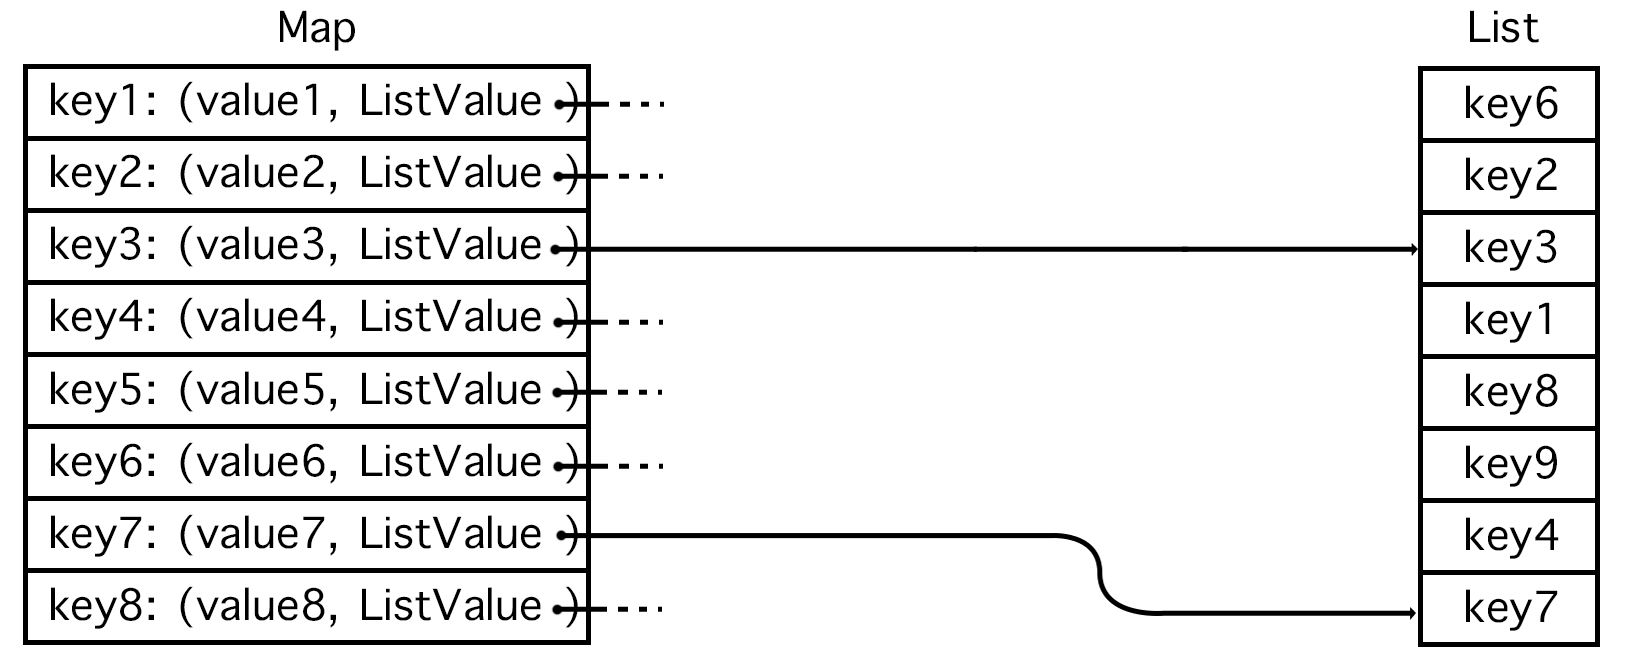
\includegraphics[width=\textwidth,height=\textheight,keepaspectratio]{img/lru.png}
  \caption{An example of an LRU with maximum size of 8. The map contains 8 items, where the key identifies the object in the map and the value is a pair of the value itself and a pointer to an element in the list. The elements of the list contain themselves the key of the object they refer to. This structure allows to perform all the needed operations in constant time. }
  \label{fig:lru}
\end{figure}

\subsubsection{LRU Warmup}\label{sec:warmup}
The main issue of using an LRU-style caching is that initially, the performance will be as bad as having no caching optimization at all. This is because until we actually have any previous calculation cached, we will still have to do all the calculations one by one. 

One possible solution for this is to employ a combination of the optimization that were presented. Since some of these optimizations work on different parts of the repartition process, we can actually use them together to have even better performance gains. For example, we can use the Hot Groups optimization, discarding the combinations of groups that are highly unlikely to be any good, and once we have the result we cache it in the LRU data structure. The Hot Groups approach would improve the performance of the system while the LRU is cold, and even when the LRU is warmed up the Hot Groups optimization would still be useful when we have a cache miss.

A possible flaw of this approach is that if one of our optimizations makes use of important approximations, then the values we store in our cache might be far from optimal; therefore, we have to be careful not to exaggerate with the approaches used. This could also be approached in a hybrid way; it is possible to use the approximation methods while the cache is empty, so that we speed up the first repartitions. Then, once the cache is full enough, we can start using the All-Combinations method whenever we have a cache-miss, so that we can start using the optimal values without having a noticeable impact on the performance of the system.

Lastly, another alternative solution to manage the bad performance of a cold LRU is to pre-load the LRU. As long as the system remains the same, we know that the cached values will still be valid. Therefore we can either store the LRU data from a previous execution, so that we can reload it before the next one, or we can pre-compute some entries of the LRU before any execution, for example entries that we expect to be likely found in our application. This would greatly reduce the drawbacks of a slow start.

\section{Optimization Tests}\label{sec:optimization-tests}
In this section we will test and compare all the different approaches to perform the repartition that were presented in the previous section. 

In particular, we will be focusing on the time it takes to complete the repartition and on the difference of the actual assignment of partitions of the different nodes of the tree.

For each case, we will use an initially empty B+ Tree of maximum slot-use, or branching factor, equal to 100. We then have variables $ITEMS$, with possible values $100'000$, $500'000$ and $1'000'000$, and $GROUPS$, with values $3, 4, 8$. The graph shape used for the groups is simmetrical, meaning that we give the same latency between all the groups.

We start each test by inserting in the B+ Tree a number of new values equal to $ITEMS$, distributed on an interval from 0 to $2\cdot ITEMS$. We then repartition, so that the statistics get reset. This avoids that these inserts affect the statistics of the repartition we actually want to test. After this first repartition, we perform, for each group, $2\cdot ITEMS$ operations, with a 50\% ratio of writes and reads. Finally we perform a second repartition, which will be timed to see how good the repartition algorithm is. Since we perform operations on the whole range of keys, it means that we will be repartitioning all the nodes at once, which is the quite rare worst-case performance.

For the last two test cases, the ones regarding the LRU caching, we perform the test differently, since it is a different type of performance optimization. We do the setup part of the test as before, but we repeat the part of performing operations and repartitioning one hundred times. This is because the LRU is an extra feature that can be paired with any of the previous algorithms, and its usefulness only shows once we have performed multiple repartitions.

% [put picture that shows client loads/skews during tests]
% \begin{figure}[!htb]
%   \centering
%   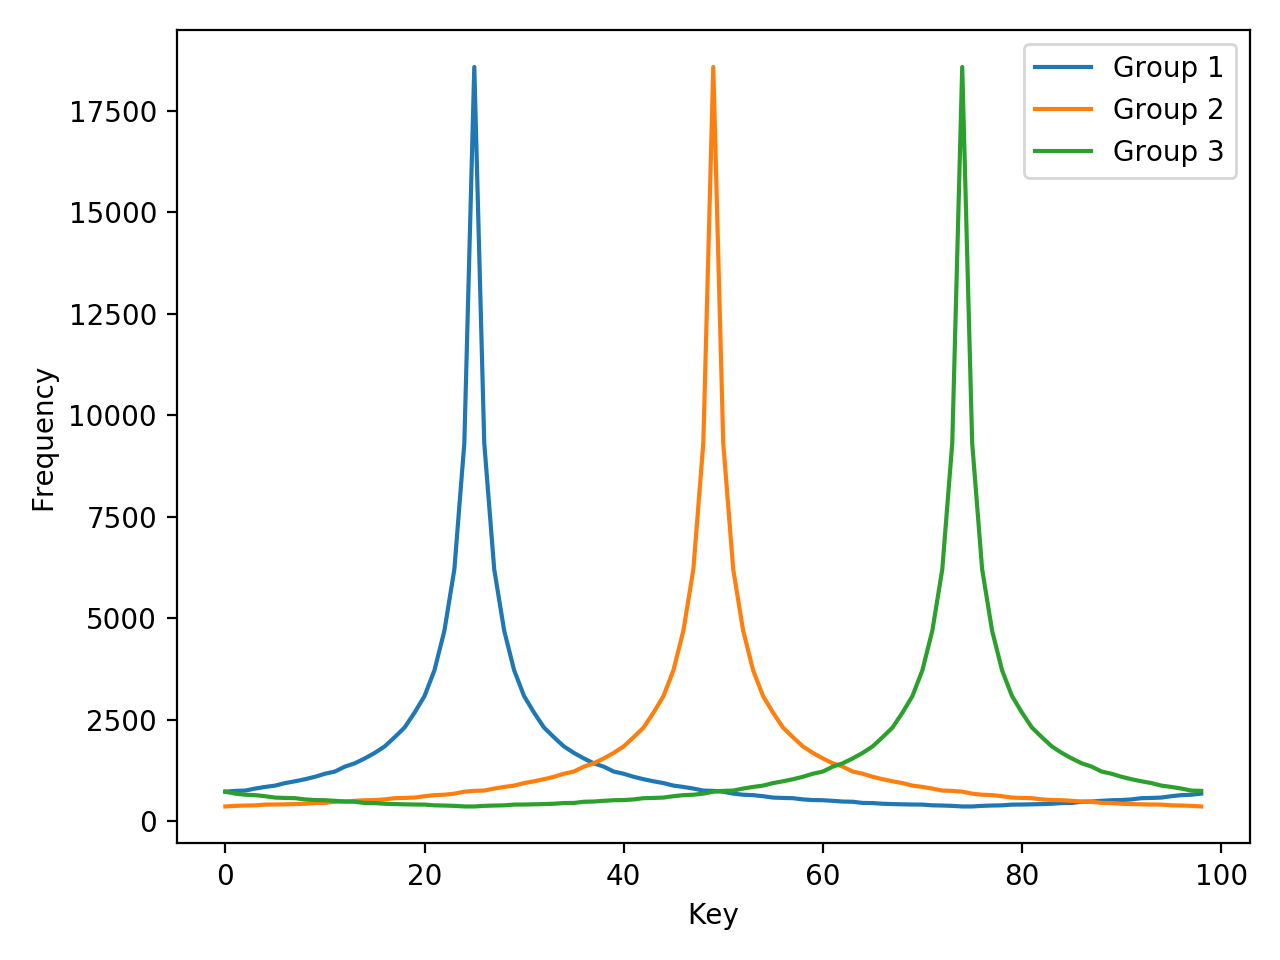
\includegraphics[width=\textwidth,height=\textheight,keepaspectratio]{img/clients_loads.png}
%   \caption{A visualization of the distribution of clients operations from the different groups and regions.}
%   \label{fig:all}
% \end{figure}

\clearpage
\subsection{All-Combinations}\label{sec:All-Combinations}
This scenario will be used as a benchmark against which we will compare all the other algorithms to. Since in this case we are considering all the possible combinations of node assignments, this algorithm will give us the best possible partitioning given a workload. At the same time it will also be the slowest one, which makes it not ideal considering that we would like to perform repartitions quite frequently, to make sure that the current partitioning matches the load of the system.

\begin{figure}[!htb]
  \centering
  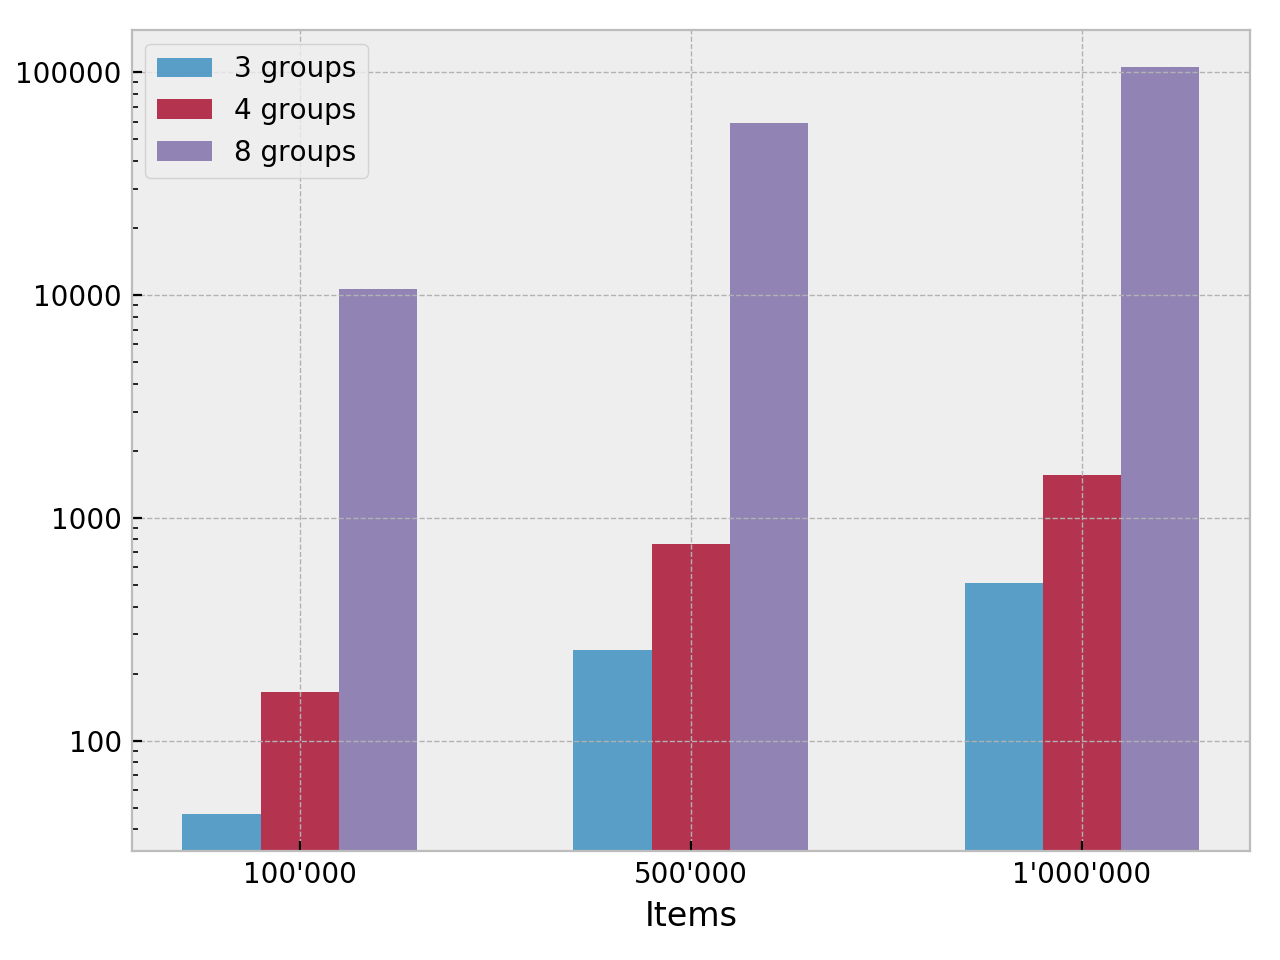
\includegraphics[width=\textwidth,height=\textheight,keepaspectratio]{img/all.png}
  \caption{The performance of the All-Combinations method with different groups and items number.}
  \label{fig:all}
\end{figure}

\subsubsection{Performance}
As we can see in figure~\ref{fig:all}, the performance slows down linearly with the number of objects in the tree, and exponentially in the number of groups, as expected. The time required to perform a total repartition becomes quickly too big, even with a relatively small tree.

\clearpage
\subsection{Fixed-Size Buckets Tests}\label{sec:Fixed-Size buckets-tests}
This approach groups the nodes in \emph{buckets} of size two, meaning that the nodes of even levels of the tree will inherit the partitions of their parent node. This reduces the number of calculations of a factor of approximately $b$, the branching factor. Therefore, we expect the repartitions to take much less time compared to the previous approach. At the same time, we know that the partitions will be approximated greatly, since we will have all the leaf nodes, the ones containing the objects, approximating their partitions to the ones of their parent node.

\begin{figure}[!htb]
  \centering
  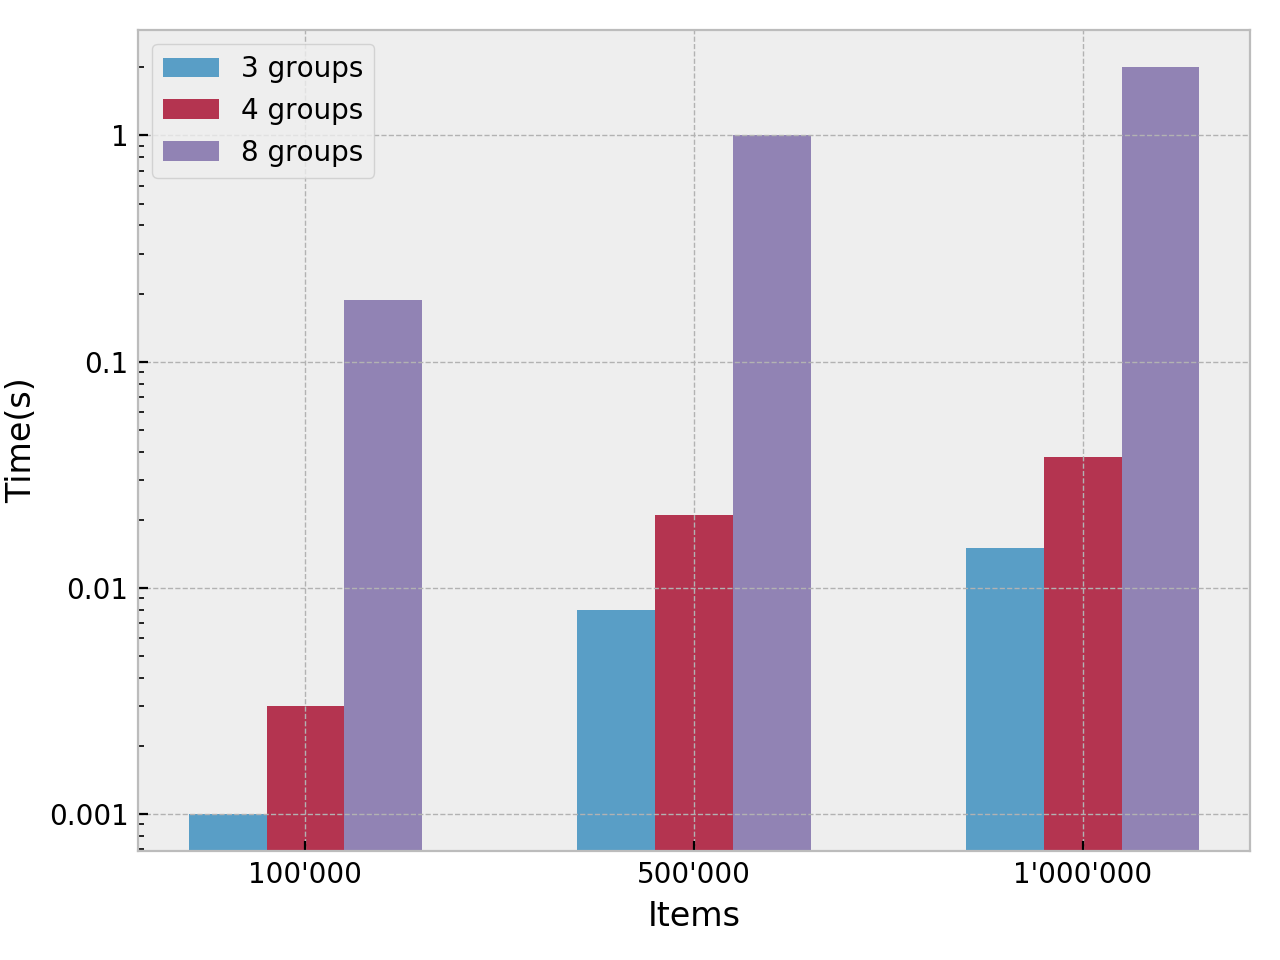
\includegraphics[width=\textwidth,height=\textheight,keepaspectratio]{img/fixed.png}
  \caption{The performance of the Fixed-Size Buckets method with different groups and items number.}
  \label{fig:fixed}
\end{figure}

\begin{figure}[!htb]
  \centering
  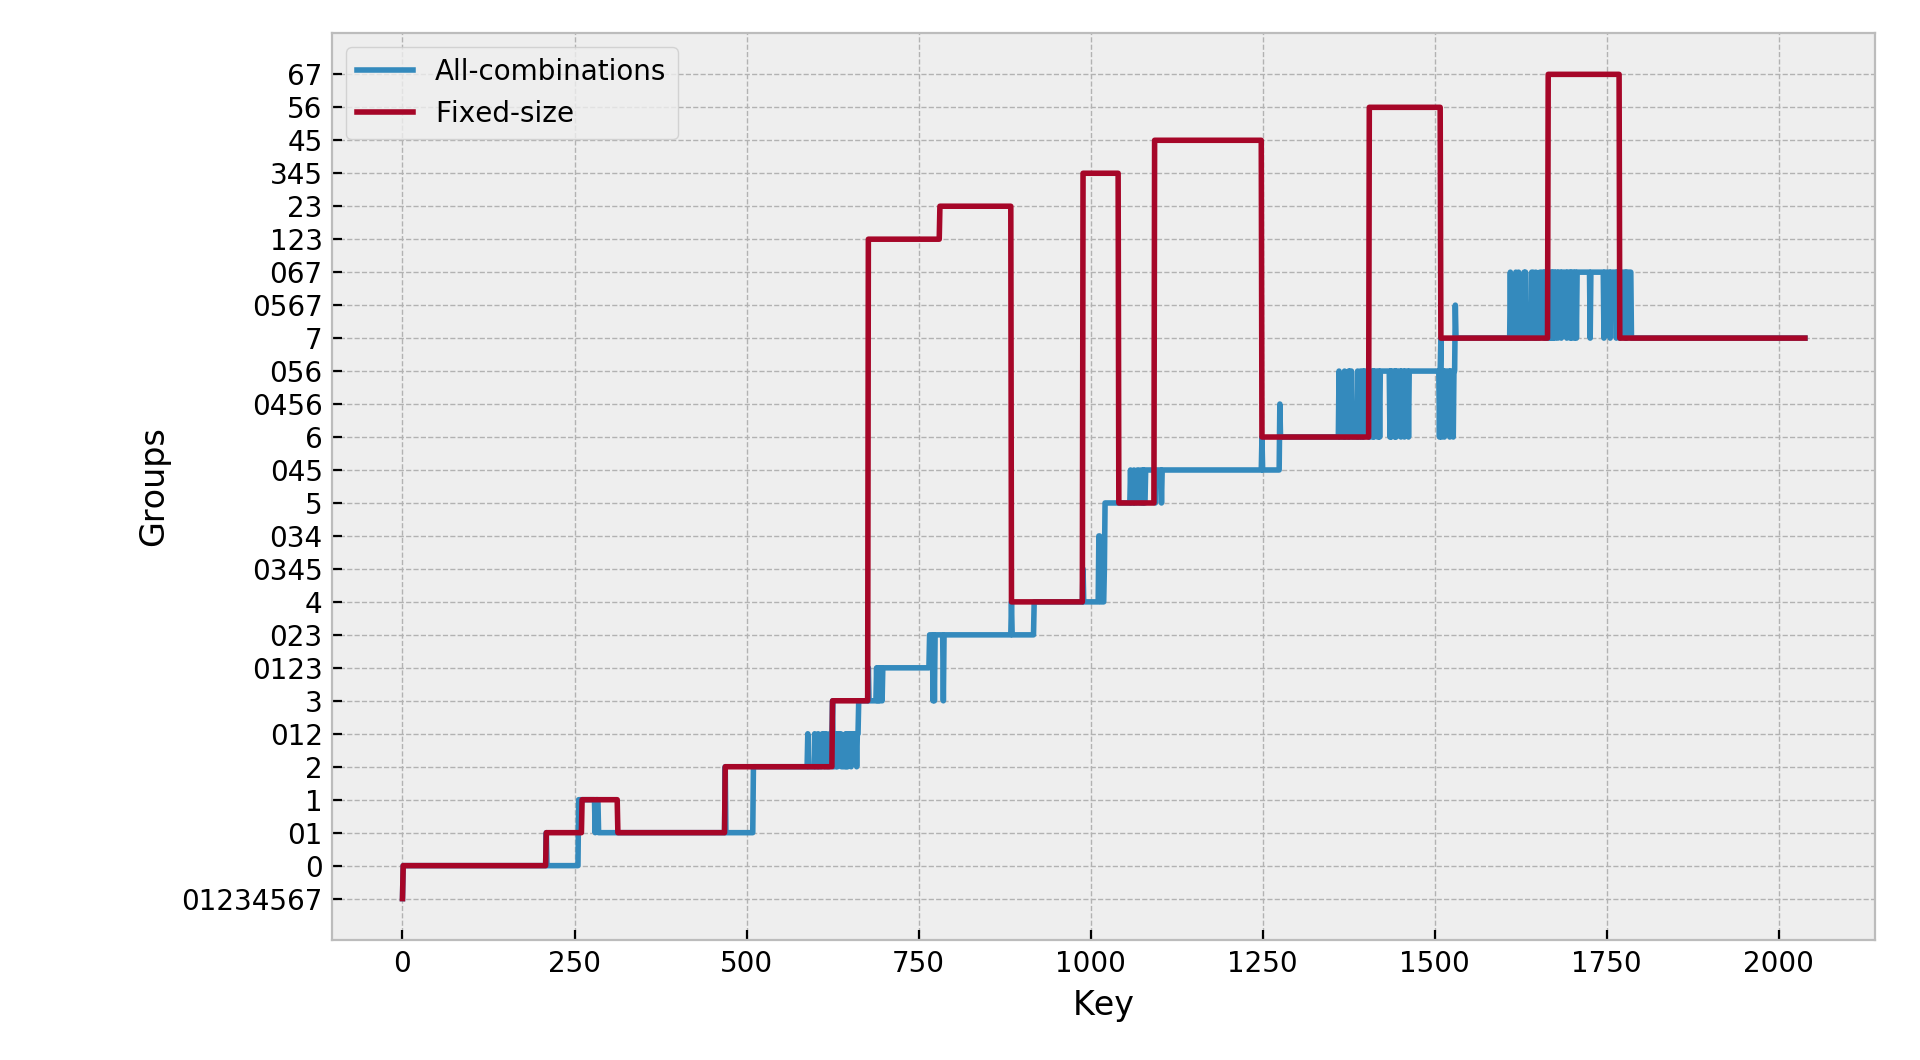
\includegraphics[width=\textwidth,height=\textheight,keepaspectratio]{img/partition_difference_fixed_all.png}
  \caption{The difference in partitions assignment between All-Combinations and Fixed-Size. The All-Combinations method shows higher variability in the key ranges where we have many operations from multiple groups. On the other hand, the Fixed-Size approach is more constant, since it decides the partitions based on aggregated statistics.}
  \label{fig:fixed-partitioning}
\end{figure}

\subsubsection{Performance}
As expected, the time required to perform the repartitions is greatly reduced compared to the previous case. When looking at the partitions of the objects, though, we see a noticeable difference in the assigned partitions. This becomes particularly apparent when we have many groups and many different loads. In the case with 8 groups and 100'000 items, out of 2039 nodes we have that 780 of those had different partitions assigned to them, which is more than one third wrongly approximated nodes. Given these results, the main reason to use this approach appears when the time of repartition is of much greater importance compared to its precision.

\clearpage
\subsection{Variable-Size Buckets Tests}\label{sec:Variable-Size-buckets-tests}
This approach is slightly more refined compared to the Fixed-Size approach, therefore we expect to see slightly better results. Since this approach generally computes more calculations compared to the Fixed-Size, we would expect the timings to be worse than the previous approach but still better than the All-Combinations one. We would also expect to see better partitions assignments.

For this method we also have to define a threshold value that is used to decide when it is worth computing the combinations for a node and when it is not. For our tests, we used as a threshold value $THRESHOLD = 0.8$, which means that if a node accounts for at least 80\% of the average expected workload of a single child node, then we will peform its calculations. The value given to this variable is a ``safe'' one chosen mostly based on previous results and we don't expect it to be ideal by any mean; still, it should be good enough to show the behavior of this approach.

\begin{figure}[!htb]
  \centering
  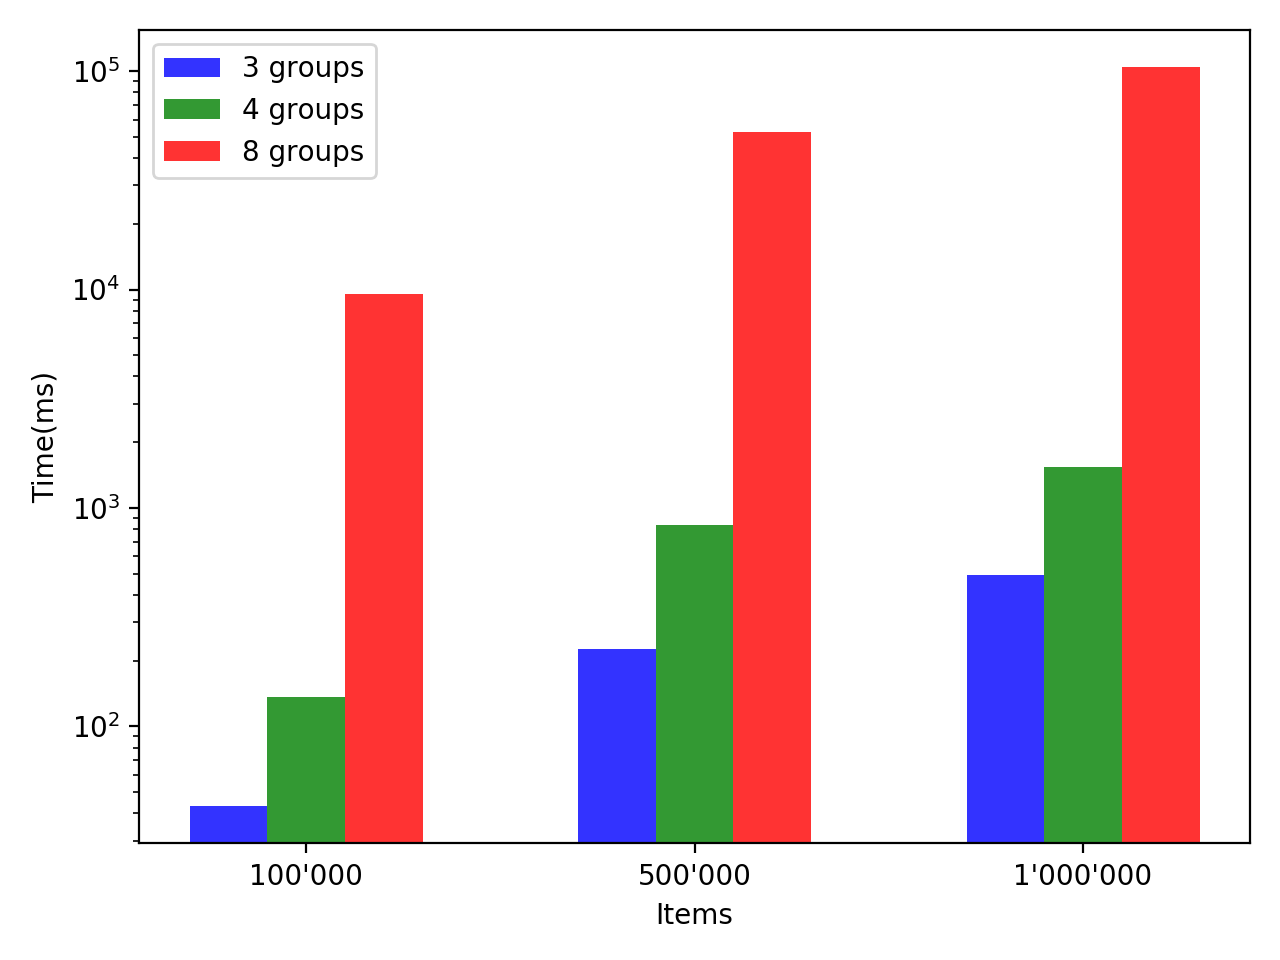
\includegraphics[width=\textwidth,height=\textheight,keepaspectratio]{img/dynamic.png}
  \caption{The performance of the Fixed-Size Buckets method with different groups and items number.}
  \label{fig:dynamic}
\end{figure}

\subsubsection{Performance}
Based on the results, this approach does not perform as well as expected: the performance is slightly better than the All-Combinations approach, but not by far, and it is much slower than the fixed-bucket approach. Also, when comparing the number of different partition assignments, we get similar results as the fixed approach, with around one third of different assignments. While this does not necessarily mean that the impact of the different assignments is the same, it does not look great. We also assume that this synthetic test might favor the Fixed-Size approach rather than the Variable-Size one, but that is just a conjecture.

\clearpage
\subsection{Hot Groups Tests}\label{sec:hot-groups-tests}
The Hot Groups approach aims at discarding combinations of groups, rather than nodes like the previous methods. This means that we expect to see an increasing gain in performance once we increase the number of groups, rather than the number of items.

In general we expect this method to perform similar to the All-Combinations one in the case with few groups, but we should also have a much more linear increment in time with the tests with more groups. We should also get better partition assignments compared to the buckets approaches, since we expect the heuristic of discarding groups to be more reliable than the ones used previously.

Like in the variable-buckets case, we have a threshold variable to set. This time it is used to decide if we should discard a group or not. We set the variable to $0.1$, which means that if a group has less than 10\% the statistics of the group with the most statistics of this node, then we will discard it. It is important to notice that the partitions assignment also depends on the ratio of reads and writes. We could use more complicate ways to calculate the threshold, taking into account the read/write ratio as well, but we preferred to keep the number of variables as little as possible to avoid complicating the tests.

\begin{figure}[!htb]
  \centering
  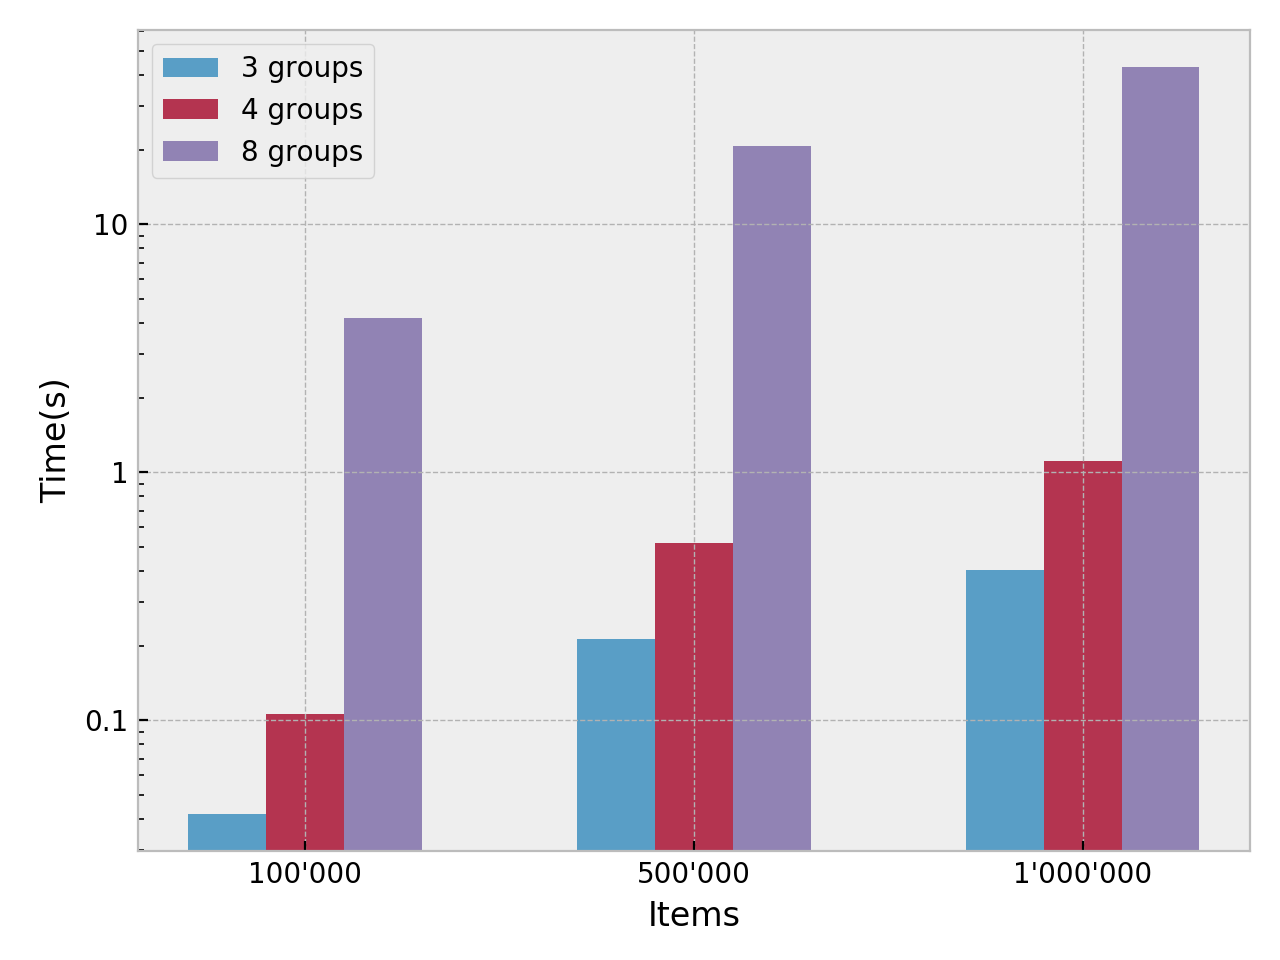
\includegraphics[width=\textwidth,height=\textheight,keepaspectratio]{img/hot.png}
  \caption{The performance of the Fixed-Size Buckets method with different groups and items number.}
  \label{fig:hot}
\end{figure}

\begin{figure}[!htb]
  \centering
  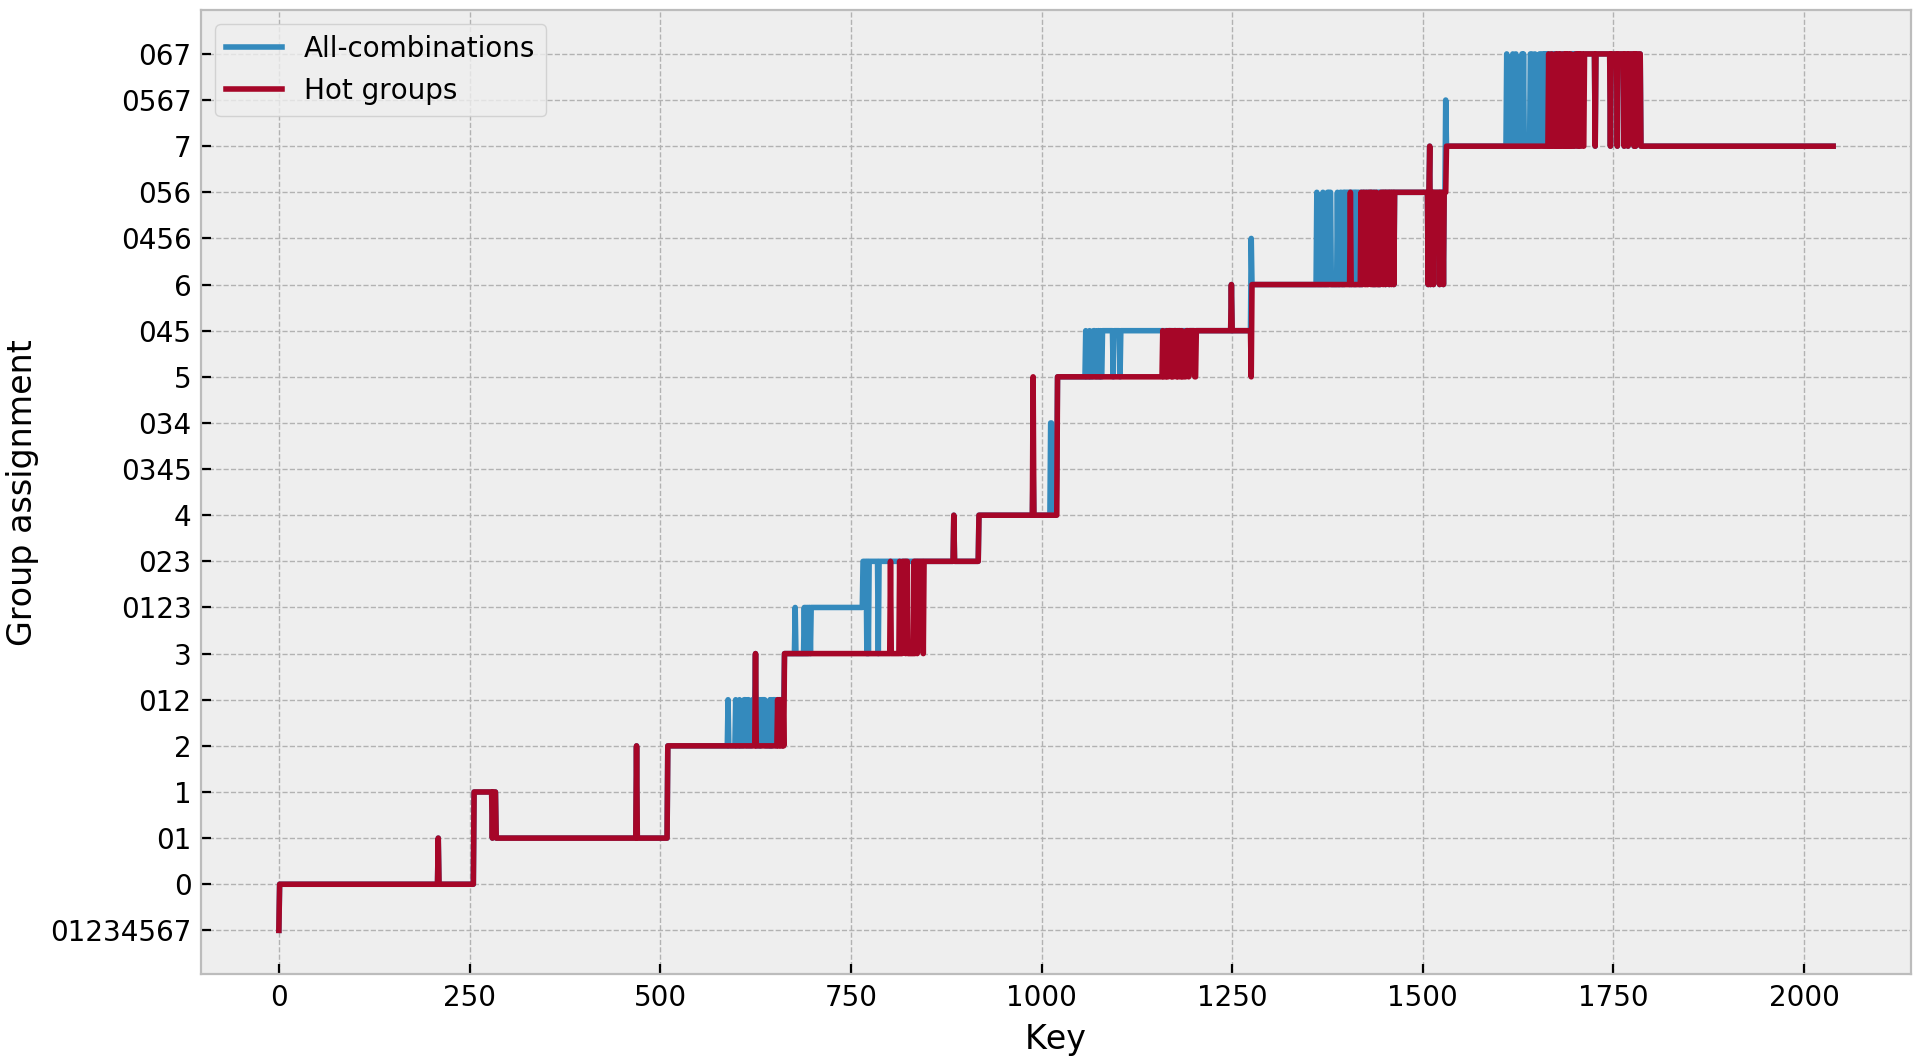
\includegraphics[width=\textwidth,height=\textheight,keepaspectratio]{img/partition_difference_hot_all.png}
  \caption{The difference in partitions assignment between All-Combinations and Hot Groups. The differences are mostly in the number of partitions that the nodes are assigned to. The All-Combinations approach assigns the nodes to multiple partitions more often than the Hot Groups. This is because Hot Groups discards the groups with few operations, therefore not considering the partitionings with multiple groups.}
  \label{fig:hot-partitioning}
\end{figure}

\subsubsection{Performance}
In this case the results of the tests are as expected. When compared to the All-Combinations case, we see that the performance in the tests with 3 groups are very similar, with the Hot Groups approach taking around 10-20\% less time. When we move onto 4 and 8 groups though the improvement is definitely more noticeable, with improvements in the order of 30-40\% and up to 65\% respectively.

Regarding the precision of the repartition, we see a difference of 380 out of 2039 nodes in the test with 100'000 items and 8 groups. The number of diffences is halved compared to the approach with buckets, which is a fair improvement. We also believe that with better, more refined choices of thresholds the number of discrepancies could be further decreased.

\clearpage
\subsection{LRU Caching Tests}\label{sec:lru-caching-tests}
As we said before, the Least Recently Used approach can be used on top of all the previous methods. For these tests, we will use it with the All-Combinations approach, to see how much we can improve upon the algorithm that gives us the optimal repartitioning. Again, since the LRU performs well once the cache is filled, this test will be performed with a series of 100 repartitions, calculating the time for each of them.

For this test, we decided to use a cache size of 1'000'000. Obviously a bigger cache would further allow improvements on the performance, at the cost of an increased load on the memory. With this cache size, we reached a usage of approximately 450MB.

We do not have a clear idea of how much the LRU will improve the results. It is hard to say if the limited size of the cache will be the bottleneck that will impede further improvements, or if we will get to the point where the mandatory calculations will become the main concern.

\begin{figure}[!htb]
  \centering
  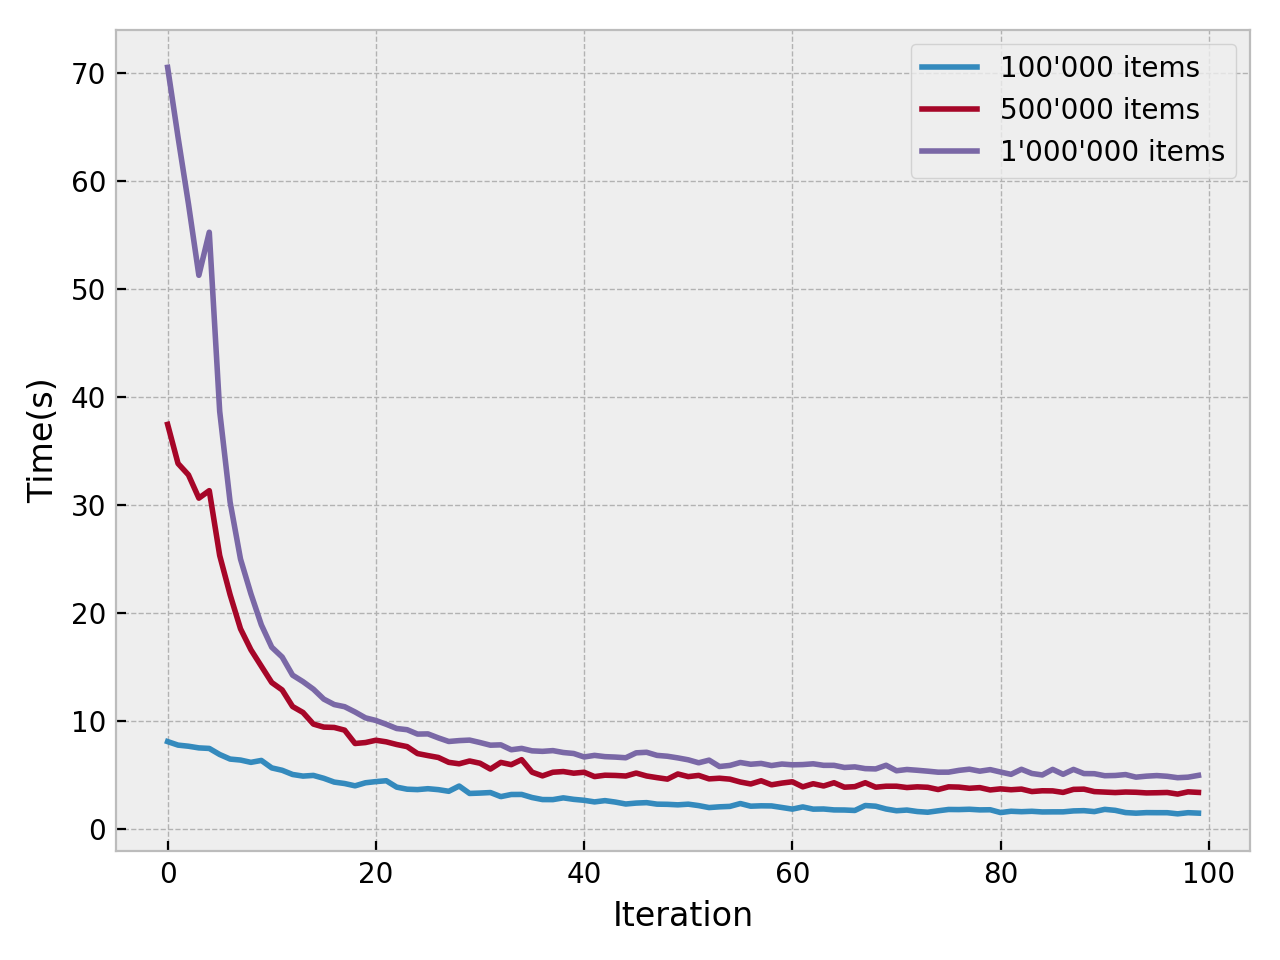
\includegraphics[width=\textwidth,height=\textheight,keepaspectratio]{img/LRU_8.png}
  \caption{The time required for 100 subsequent repartitions using the LRU and the All-Combinations method. The performance improves greatly once the LRU cache gets filled. }
  \label{fig:LRU_8}
\end{figure}

\subsubsection{Performance}
The results seem really good: in 100 repartitions the computation time decreased to $\frac{1}{10}$ of what it was initially, going below 10 seconds in the best cases. While 10 seconds is still a lot of time, we can be sure that even longer amounts of repartitions will boost the performance even more. 

It is also interesting to notice that even from the first repartition, the time was around 70 seconds, definitely less than the 105 of the approach with LRU. This shows that even with just one repartition we have a noticeable amount of cache-hits. This most likely happens with close objects, that have a high chance of having similar workloads thanks to their high locality.

\clearpage
\subsection{LRU with Hot Groups}\label{sec:lru-hot-groups}
We will now test the performance of the LRU combined with the Hot Groups approach; the idea is that the Hot Groups will make up for the slow initial repartitions when the LRU cache is empty. Once the cache is filling up the performance should increase rapidly, giving us good approximations of the repartitions thanks to the Hot Groups. 

\begin{figure}[!htb]
  \centering
  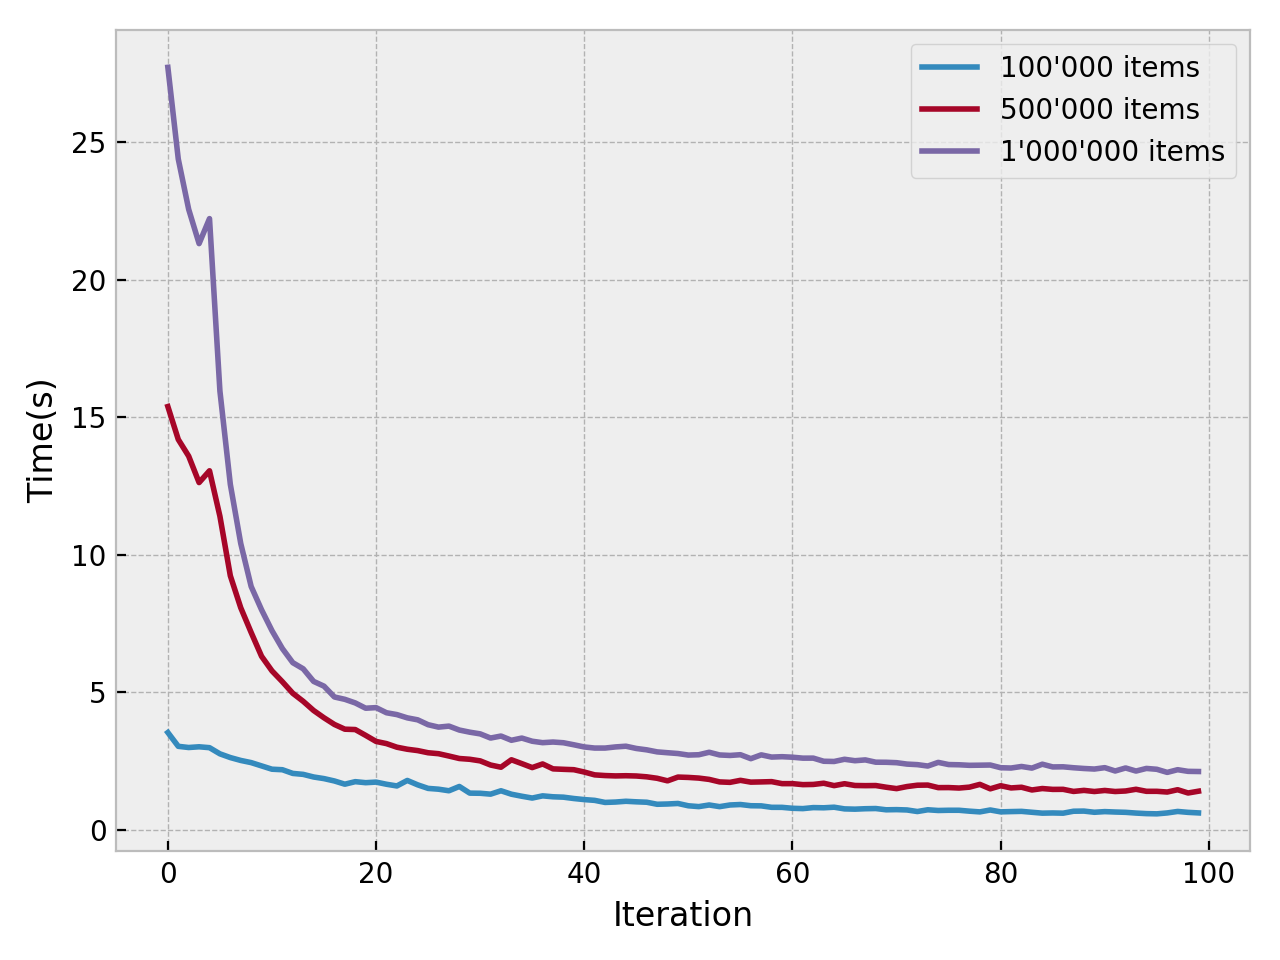
\includegraphics[width=\textwidth,height=\textheight,keepaspectratio]{img/LRU_8_hot.png}
  \caption{The time required for 100 subsequent repartitions using the LRU and the Hot Groups method. The shape of the plots is similar to the one with All-Combinations, but all the curves are lower, meaning that this always takes less time than the previous one, at the cost of precision.}
  \label{fig:LRU_8_hot}
\end{figure}

\subsubsection{Performance}
The results are in line with our expectations; the timing are consistently lower than the previous LRU test, both at the beginning and at the end. The percentage decrease in computation time is similar to the percentage decrease we saw without the LRU.

\clearpage
\section{Repartition Results Evaluation}\label{sec:repartition-results-evaluation}
Based on the results, we can draw some conclusions on the quality of the various methods compared against each others. 

The All-Combinations approach gives us the optimal partition assignments to obtain minimum average latency, but in the case of a repartition of relevant size the time it takes is definitely too long. the combinations with 8 groups take from 10.5 to 105 seconds; we definitely cannot stop the execution of the system for that long, unless we perform repartitions very infrequently.

The Fixed-Size buckets approach is on the other end of the spectrum; really short computation times, but it leads to great approximations in the repartition. Still, with the 8 groups, 1 million items workload, the repartition time was 2 seconds compared to 105, so it looks at least usable as a starting approach or when timing is a great concern.

The Variable-Size buckets turned out to be rather disappointing. Computation times are slightly better than the All-Combinations approach, but a number of ``wrong'' assignments comparable to the Fixed-Size one. We still believe that it was a bad test case for this method; perhaps different loads and different tresholds would lead to better results. Yet, we cannot feel encouraged to use this method given the results we have at hand.

The last computation optimization, the Hot Groups, performed quite well. In particular, the computational times with 8 groups are less than half compared to the All-Combinations, which is a nice improvement, and the number of wrong assignments is half of the Fixed-Size buckets. In general, it looks like the most balanced optimization. This method is also particularly useful because it targets the number of group combinations, which quickly becomes an issue when we have many groups.

The results get interesting when paired with the caching system. Even with the slowest computation method, the biggest workload goes from 105 seconds to less than 10 seconds in just 100 repartitions. When paired with a faster computation method, like Hot Groups, it goes even below 3 seconds. As a matter of fact, when we tried with 1000 repartitions, at the 500th one the time was around 1 second, plateauing at around 600, with around 950ms on average, and a memory usage of 1GB.
By comparison, the one without Hot Groups reached a plateau at 400 repartitions, with an approximate time of 2-2.5 seconds per repartition.

In conclusion, it looks like the way to go is definitely by exploiting the LRU caching, and pairing it with a different computational method depending on how time and precision are important for our system.

\clearpage
\section{GeoPaxos Tests}\label{sec:geopaxos-tests}
Now that we have asserted the performance of the various approaches, we will run a more in-depth suite of tests with various types of settings, to simulate how the B+ Tree on top of GeoPaxos behaves in different situations.
\subsection{Tests Setup}\label{sec:tests-setup}
It is quite hard to come up with tests that give us realistic workloads, but we believe that the tests we discuss in this section should give a decent idea of the cases where it performs better and the cases where it could be improved. While we could have included more combinations of tests in the report, we believe that it would have become overwhelming and more confusing rather than adding any useful extra information.

The tests have a range of variables to be set, including:
\begin{itemize}
  \item \textbf{Number of clients (per destination group)} The number of clients that are connected to each group of the system, e.g. the number of clients for each region.
  \item \textbf{Number of threads (per client)} The number of threads used for each client entity. Increasing the number of threads boosts the maximum throughput of a single client, but each client still has to receive a reply to a previous message sent before sending a new one. During testing we keep the value in a way so that the performance of the clients is consistent, and we use a high number of threads to limit the bottleneck of message handling so that we can focus the performance on the latency of the communications.
  \item \textbf{Number of outstanding messages} The maximum number of requests that a client can have on-hold at once. If set to one, a client can only send a second request after it has received an answer for the first request.
  \item \textbf{Number of items} The total number of items, or keys, on which the clients can perform operations.
  \item \textbf{Maximum throughput (msgs/s)} The maximum number of messages that a client can send in a second.
  \item \textbf{Range of operations} The interval of keys that the client is going to perform operations on. This usually corresponds to the total number of items, but the beginning and end of the range will be shifted depending on the region of the client.
  \item \textbf{Ratio of operations} The ratio of read and write operations performed by the client.
  \item \textbf{Skew alpha} The skew of the zipf[link] function that defines the frequency of operations on the range of keys (see Figure ~\ref{fig:skews}).
\end{itemize}

All the clients behave in the same way. Once started, they send messages to the replica that they are connected to (at a rate depending on the variables defined above), and waits for the replies. There are some possible behaviors of clients that may not seem important at first, but that are quite important to keep under control to avoid unexpected or unwanted results from the tests.

One interesting such case happens when a client, because of a time period with a high throughput, has a repartition that puts a lot of objects in the region where he is at. This leads to his operations having even lower latency than before, which leads to even higher throughput than before, leading to a situation where he will be the most performant client exactly because it was performant in the past. To handle this, we have two variables: the maximum throughput, that makes it so that after a certain point, the client cannot send more messages than a certain threshold. Furthermore, we can increase the number of outstanding messages; while this sounds counterintuitive, having a higher outstanding limit allows slower clients to send more messages without having to wait for replies of past messages, limiting the gap between fast and slow clients. Both these settings (maximum throughput and outstanding messages) could be realistic behaviours, too: common clients may not have the fastest internet speed, therefore limiting their maximum throughput, and not all requests may be dependent on each other, therefore a client will not have to wait a reply for all messages before sending new ones.

The tests will proceed as follows. After having started all the rpelicas, we will start all the clients at the same time. We will perform the first repartition after 1 minute, since the system will initially be slow and without any previous statistics to use. After that first one repartition, we will perform further repartitions every 30 seconds. Every test will run for a total of approximately 5 minutes, during which 8 repartitions will be performed.

For each region, we will have 10 clients (with multiple threads for each client, to make sure that we maximise its performance), with the distribution of operations dependant on the test. The clients will also have a limited throughput set to 50 messages per second. While this limits the maximum throughput of the system, it is important to remember that we do not want to test the maximum throughput, but only minimize the average latency. Furthermore, limiting the throughput simulate clients which do not have server-like performance, and it avoids that just a few clients monopolize the system, giving all the other clients an even opportunity to use the system.

\begin{figure}[!htb]
  \centering
  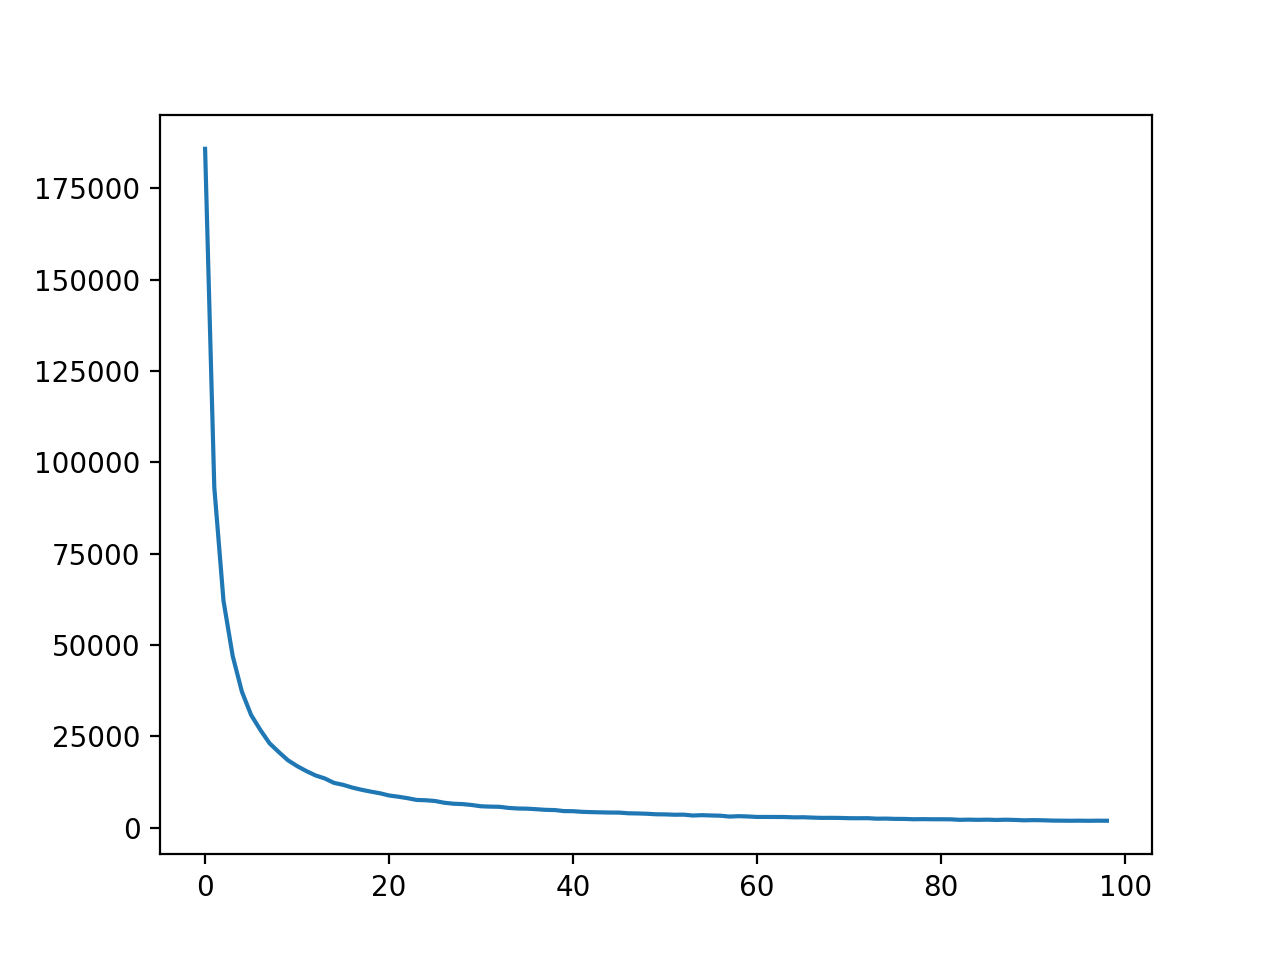
\includegraphics[width=0.49\textwidth,height=\textheight,keepaspectratio]{img/skew-alpha1.png}
  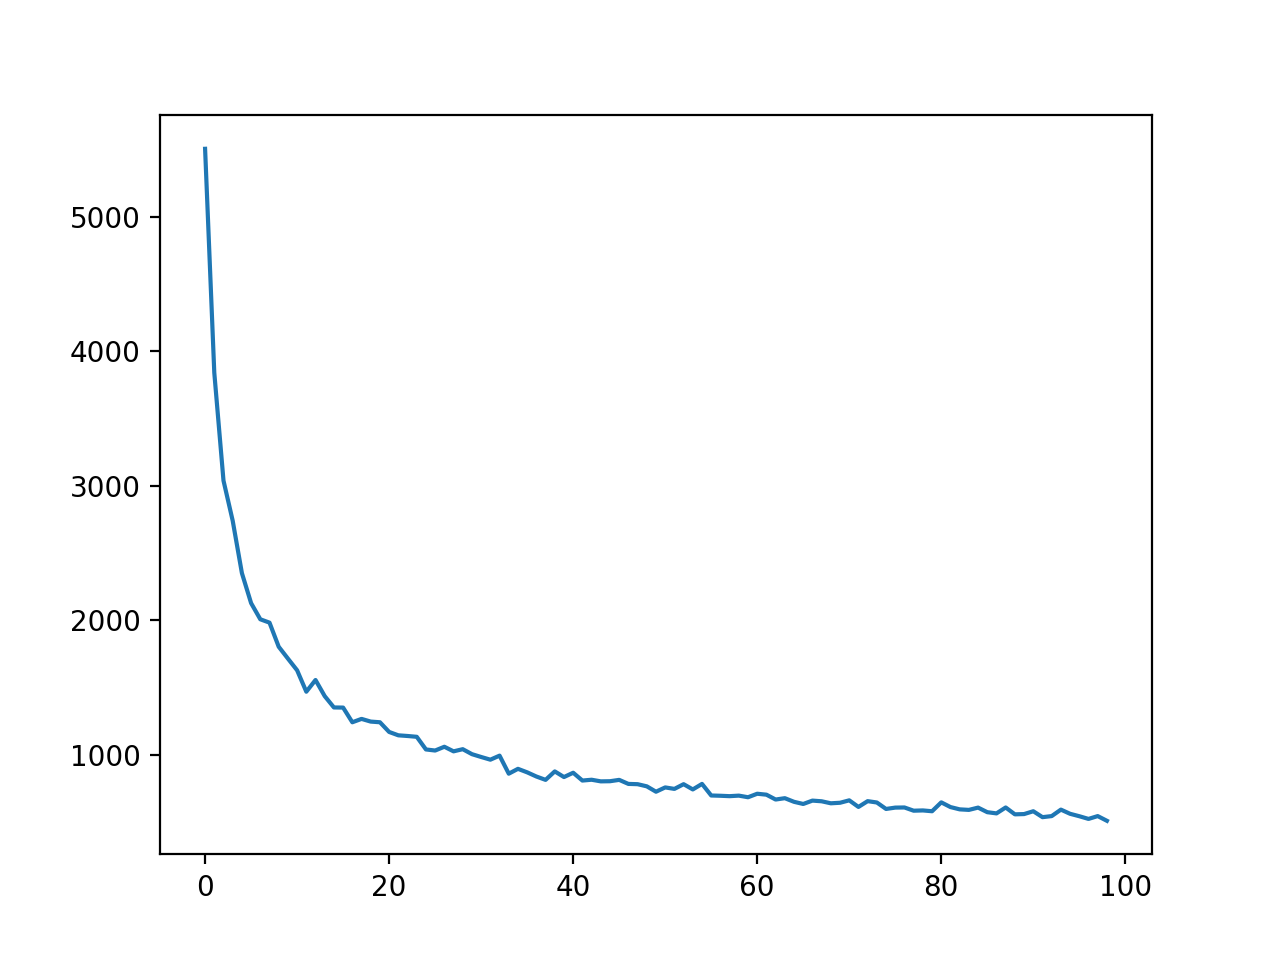
\includegraphics[width=0.49\textwidth,height=\textheight,keepaspectratio]{img/skew-alpha05.png}
  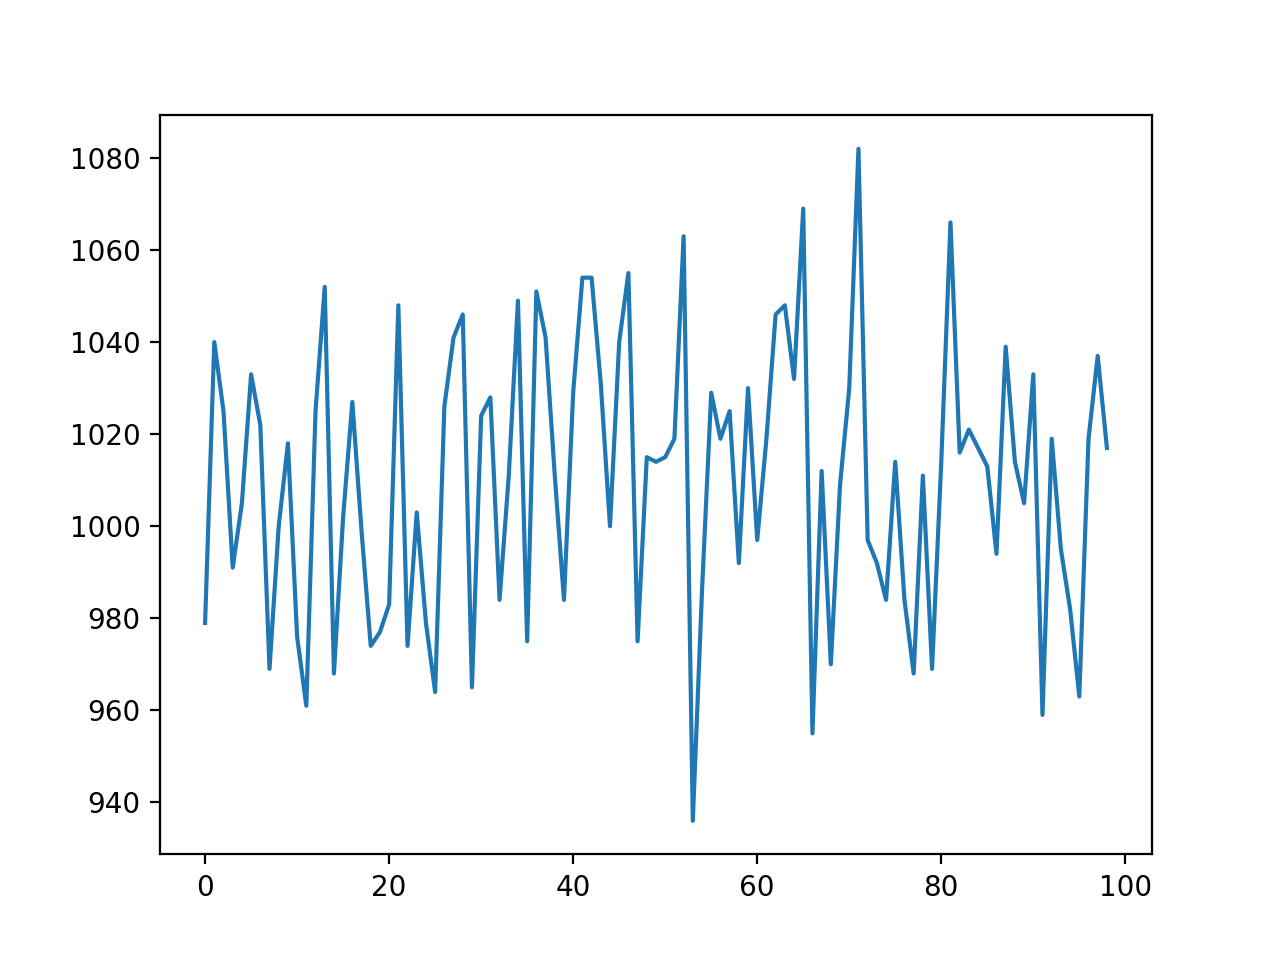
\includegraphics[width=0.49\textwidth,height=\textheight,keepaspectratio]{img/skew-alpha0.png}
  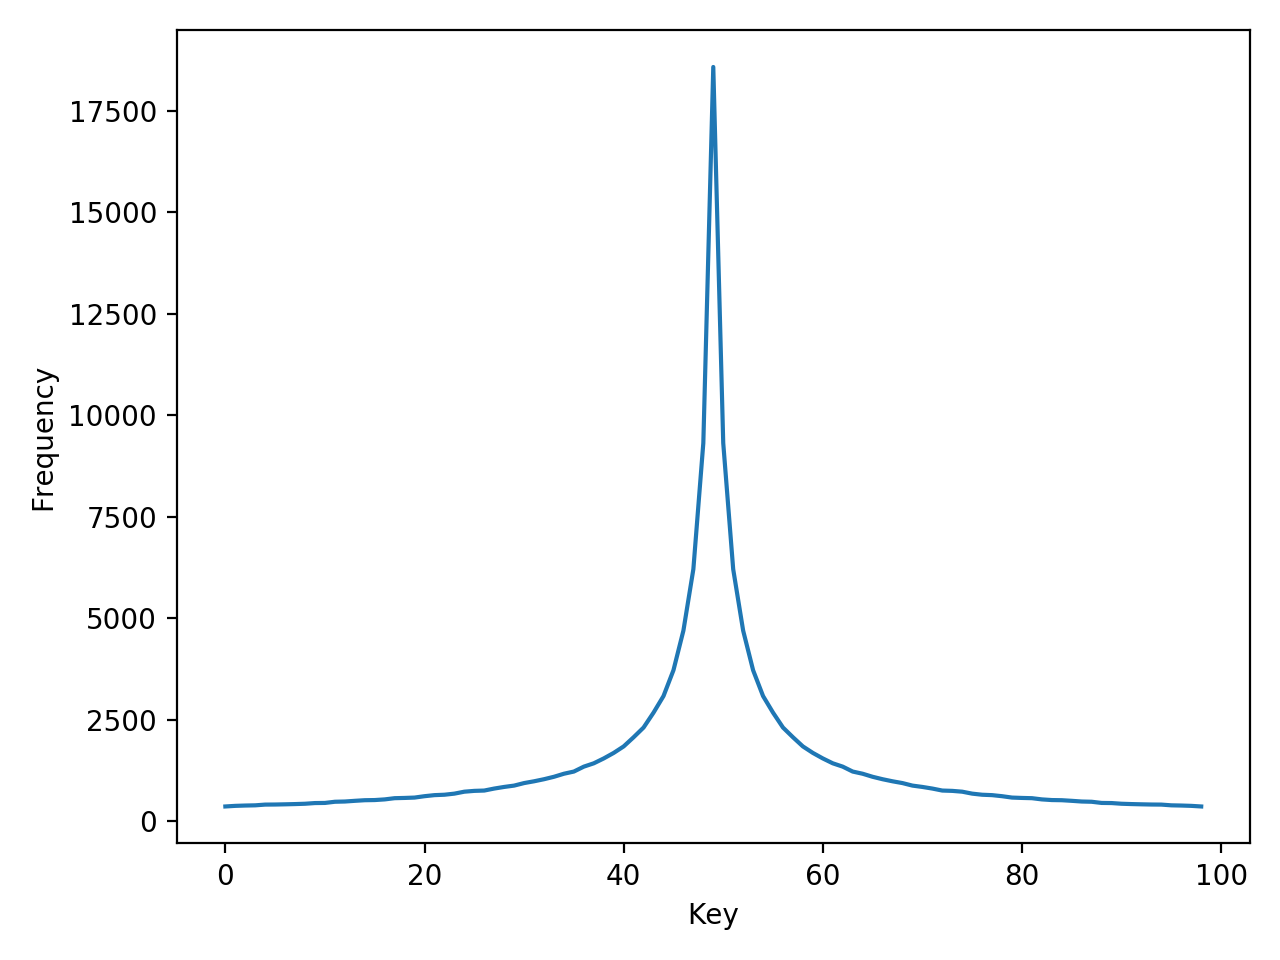
\includegraphics[width=0.49\textwidth,height=\textheight,keepaspectratio]{img/skew-alpha1smooth.png}
  \caption{ The four plots show the different skew distributions using different alpha values. Top-left: $alpha = 1$, Top-right: $alpha = 0.5$, Bottom-left: $alpha = 0$, Bottom-right: $alpha = 1$ with smooth setting. The first three are quite self-explanatory, with the curve getting flatter and flatter the more we get close to zero. With the smooth curve it is important to notice that we are cutting the original curve in half, therefore the distribution will look slightly different compared to a non-smooth one with the same alpha.}
  \label{fig:skews}
\end{figure}


Note that the zipf skew used in the tests is a slightly modified one, which we call \emph{smooth skew}, which is simply a skew that is mirrored after the peak point of the curve. This is because otherwise, there would be a really big difference in load between the maximum point of the curve and the minimum one, even though from a key point of view they are off by one, showing very low locality.

The particular setups that we will test are four types of client behaviors, that we call local-skewed, global-skewed, constant and variable. For each of these, we will run tests with read/write ratios of 50, 90,95,99 (where 99 means 99\% of operations are going to be reads). For the tests we will have three groups; the tests will be run on a local cluster of machines, but with with simulated latencies between the replicas. These latencies were measured during the testing of GeoPaxos[cite] while it was been tested on Amazon EC2 servers, and it was seen that the results of the real geographically distributed machines on EC2 nodes and the results with the simulated latencies were fairly similar. The simulated locations for the datacenters are in Tokyo(JP), California(CA) and Ireland(EU), with calculated latencies between the regions in table~\ref{tab:latencies}. For the Paxos entities, the datacenters in each region contain 3 acceptors and one replica co-located with one of the acceptors. The latencies measured inside a datacenter were negligible, in the order of 1ms.


\begin{table}[!htb]
  \centering
  \begin{tabular}{l l l l}
    \hline
    & \textbf{EU} & \textbf{CA} & \textbf{JP} \\
    \hline
    \textbf{EU} & 1 & 145 & 215 \\
    \textbf{CA} & 145 & 1 & 145 \\
    \textbf{JP} & 215 & 145 & 1 \\
    \hline
  \end{tabular}
  \caption{The latencies used in our local cluster of machines used to simulate geographically distant datacenters, placed in Ireland(EU), California(CA) and Tokyo(JP).}\label{tab:latencies}
\end{table}

[put image similar to GeoPaxos that shows replicas and latencies]

\clearpage
\subsection{local-skewed}\label{sec:local-skewed}
In a geographically distributed environment, one of the possible types of workloads that we expect to see is a workload that depends on the geographic location of the clients themselves. For example, we expect that the users from Europe will access data object related to news about Europe rather than America or Asia. Another similar example can be seen in social networks, where geographically close people have a higher chance of being connected.

Following this logic, the test we perform has three groups of clients in different regions that perform similar operations, but the distributions are shifted, so that they each focus on different key ranges. Figure ~\ref{fig:local-skewed-loads} shows a similar workload.

\begin{figure}[!htb]
  \centering
  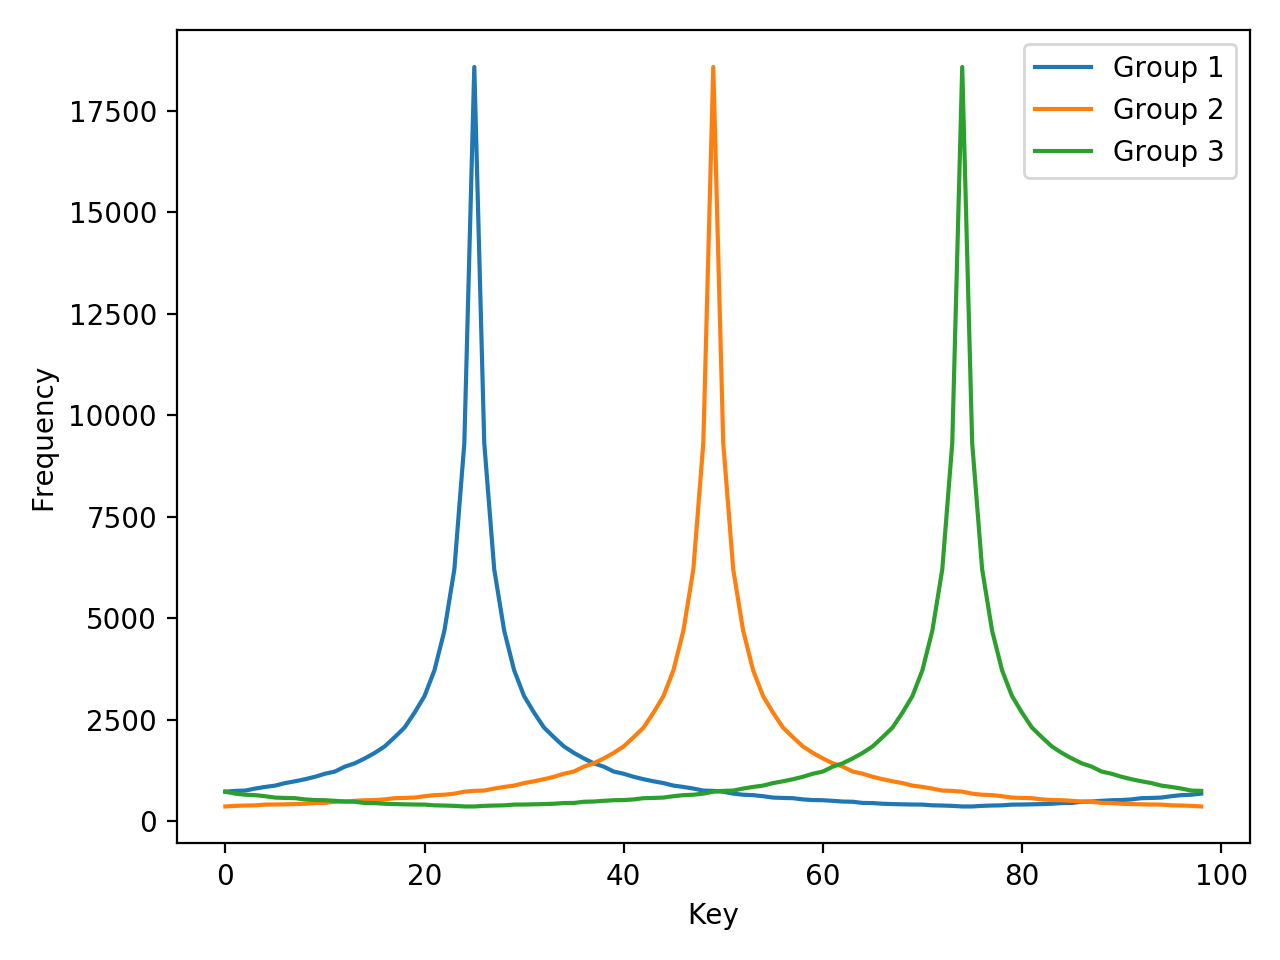
\includegraphics[width=\textwidth,height=\textheight,keepaspectratio]{img/clients_loads.png}
  \caption{ local-skewed-loads }
  \label{fig:local-skewed-loads}
\end{figure}

Because this situation is the ideal case for GeoPaxos, we expect the performance to grow quite steadily after a few repartitions. This is because the shifted loads allow to assign the different areas to the different groups quite easily, allowing us to perform all the single group operations with almost no latency involved in the communications.

\begin{figure}[!htb]
  \centering
  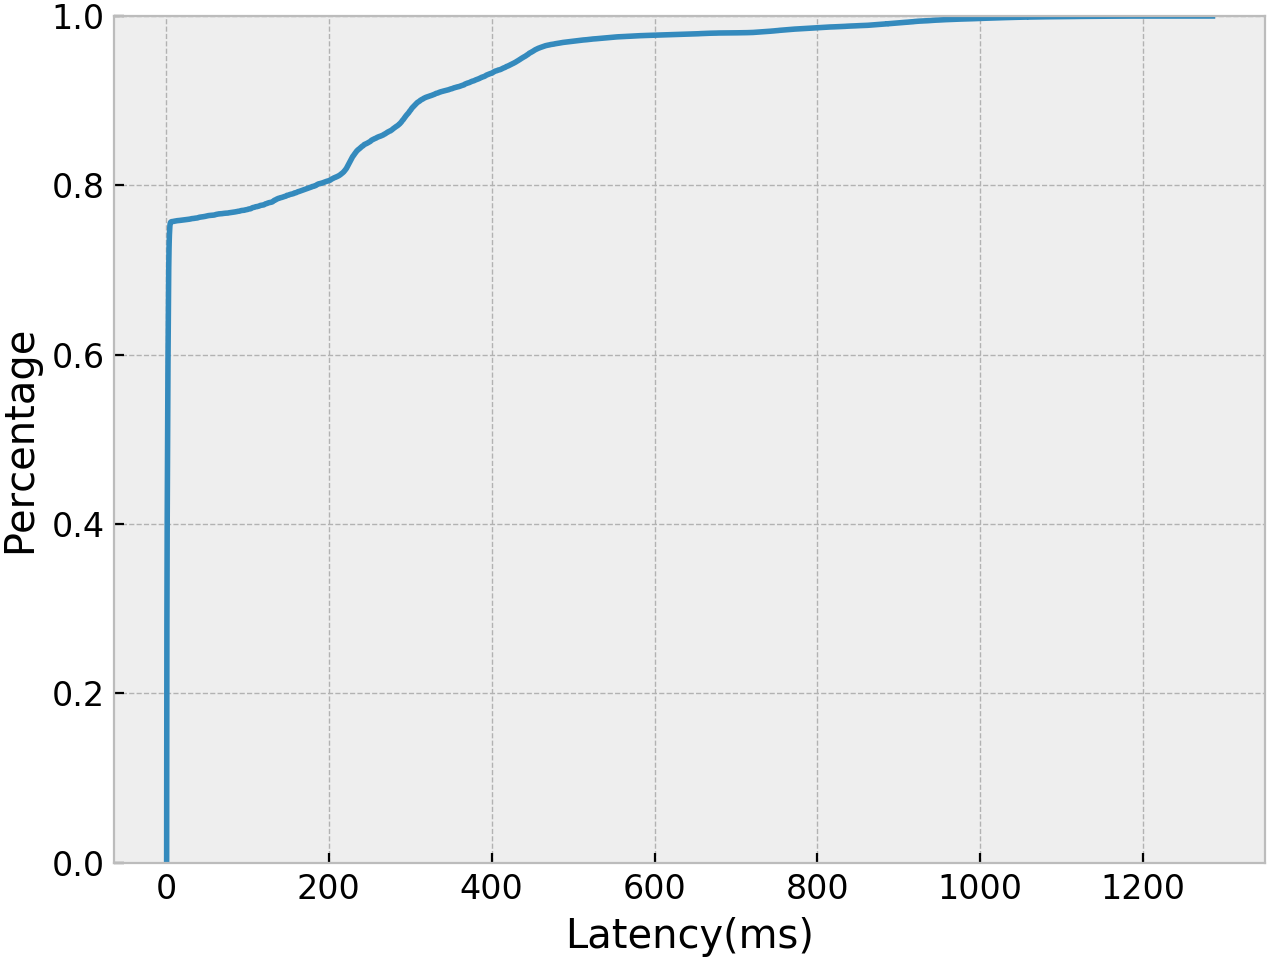
\includegraphics[width=0.49\textwidth,height=\textheight,keepaspectratio]{img/local50_lat.png}
  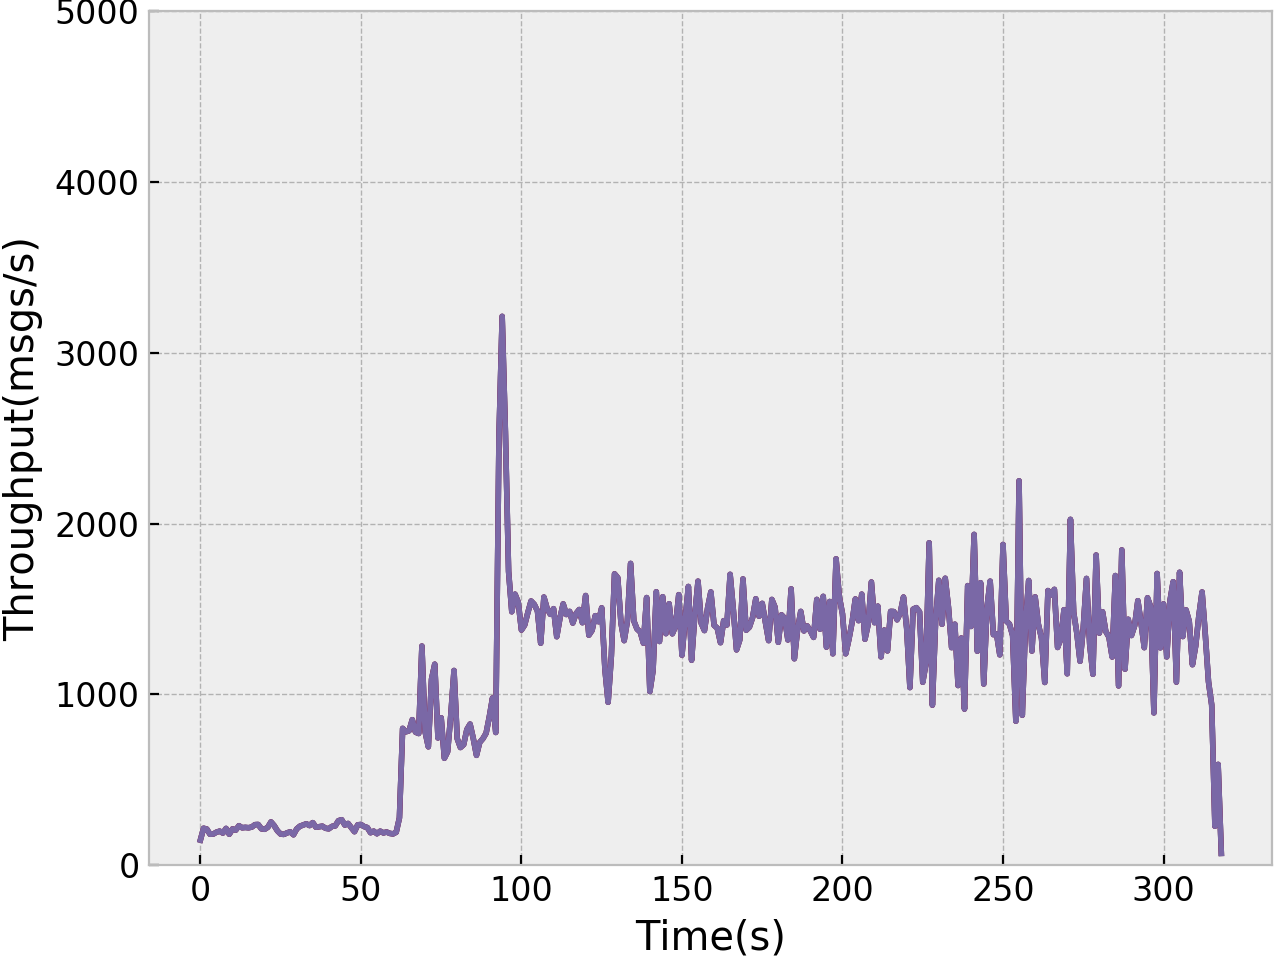
\includegraphics[width=0.49\textwidth,height=\textheight,keepaspectratio]{img/local50_tp.png}
  \caption{ 50\% reads }
  \label{fig:local50-performance}
\end{figure}

\begin{figure}[!htb]
  \centering
  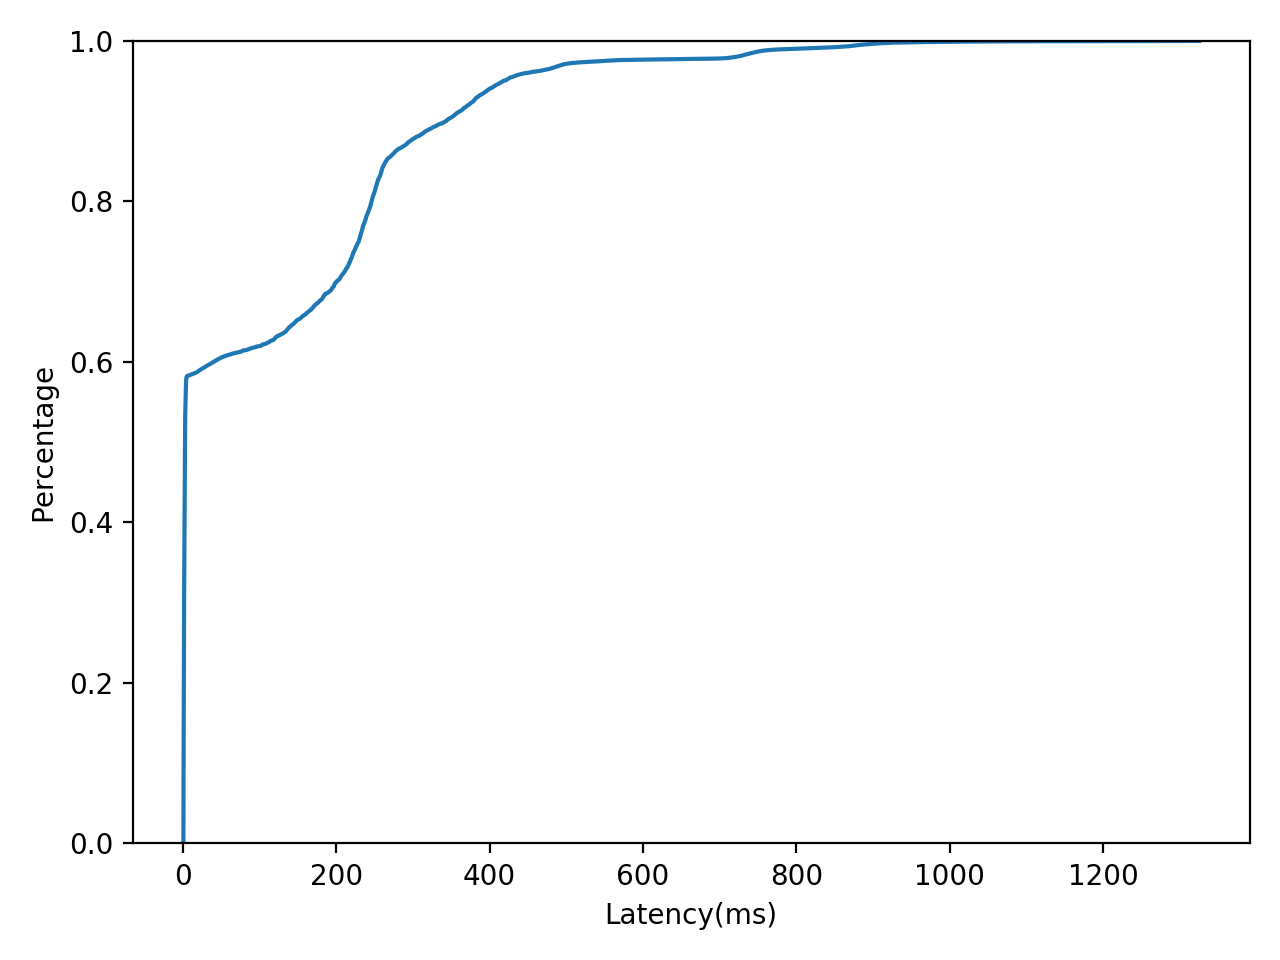
\includegraphics[width=0.49\textwidth,height=\textheight,keepaspectratio]{img/local10_lat.png}
  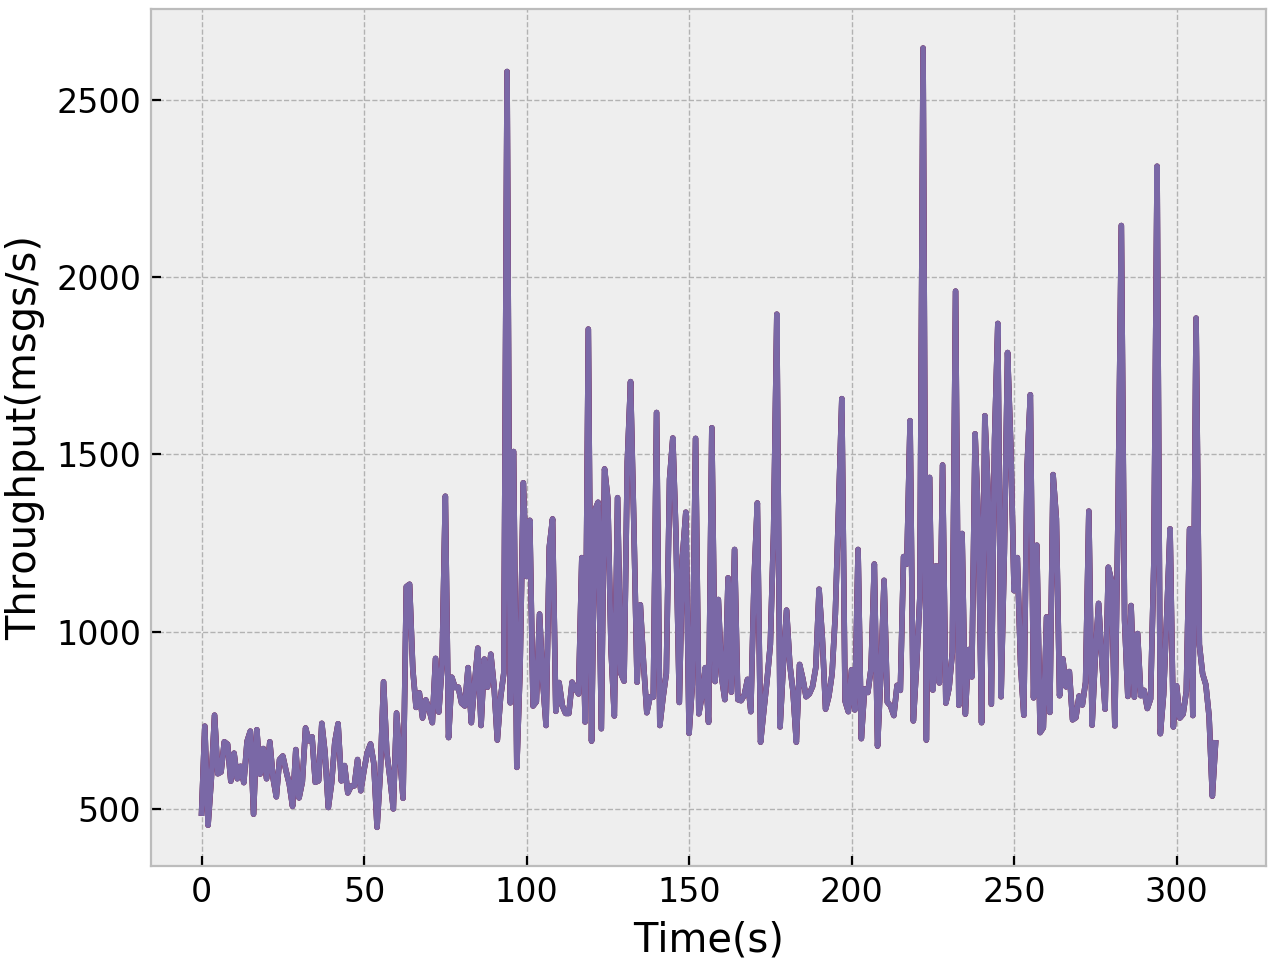
\includegraphics[width=0.49\textwidth,height=\textheight,keepaspectratio]{img/local10_tp.png}
  \caption{ picture that shows client loads }
  \label{fig:local10-performance}
\end{figure}

\begin{figure}[!htb]
  \centering
  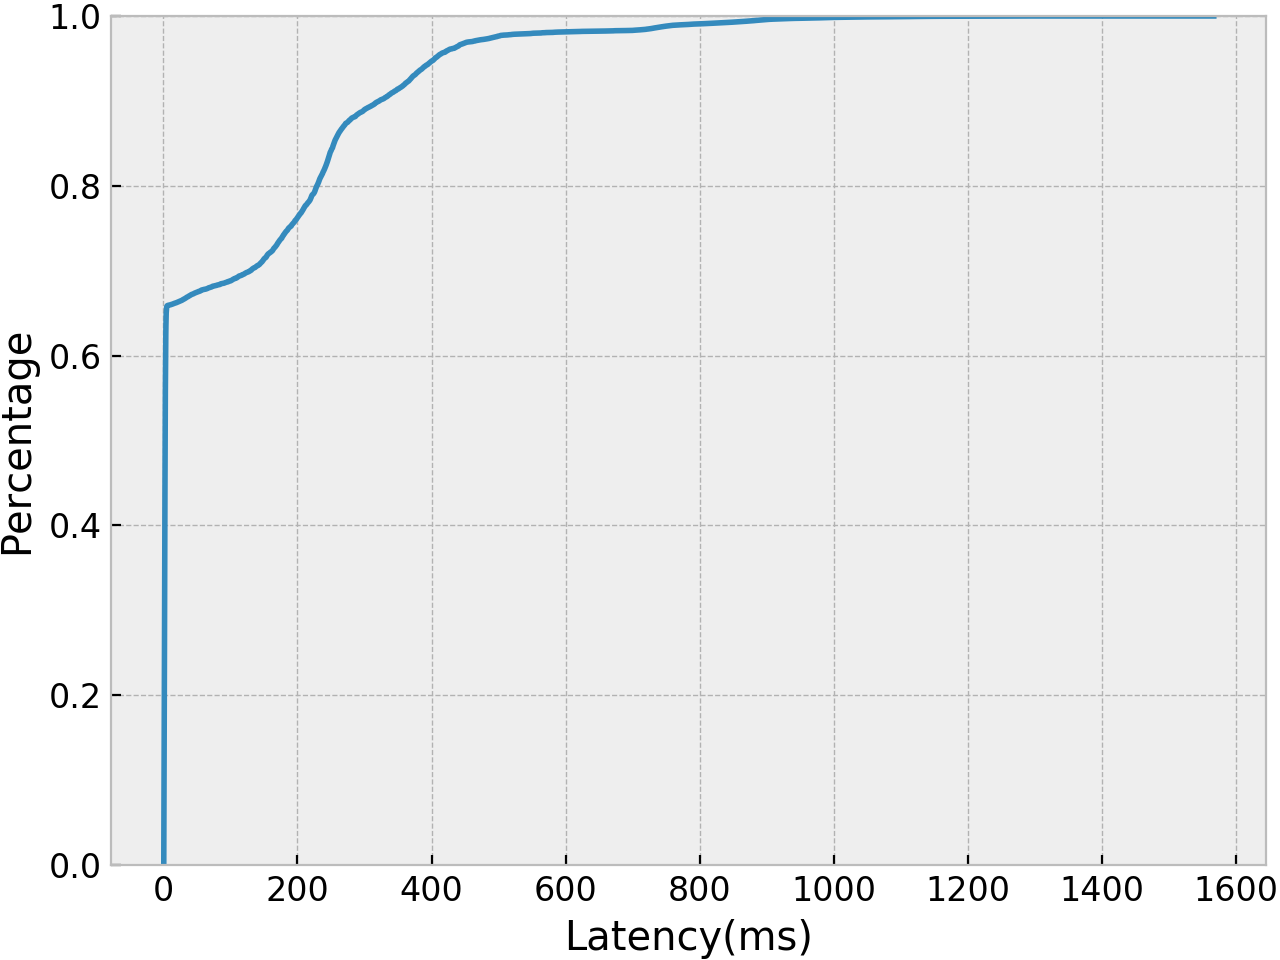
\includegraphics[width=0.49\textwidth,height=\textheight,keepaspectratio]{img/local5_lat.png}
  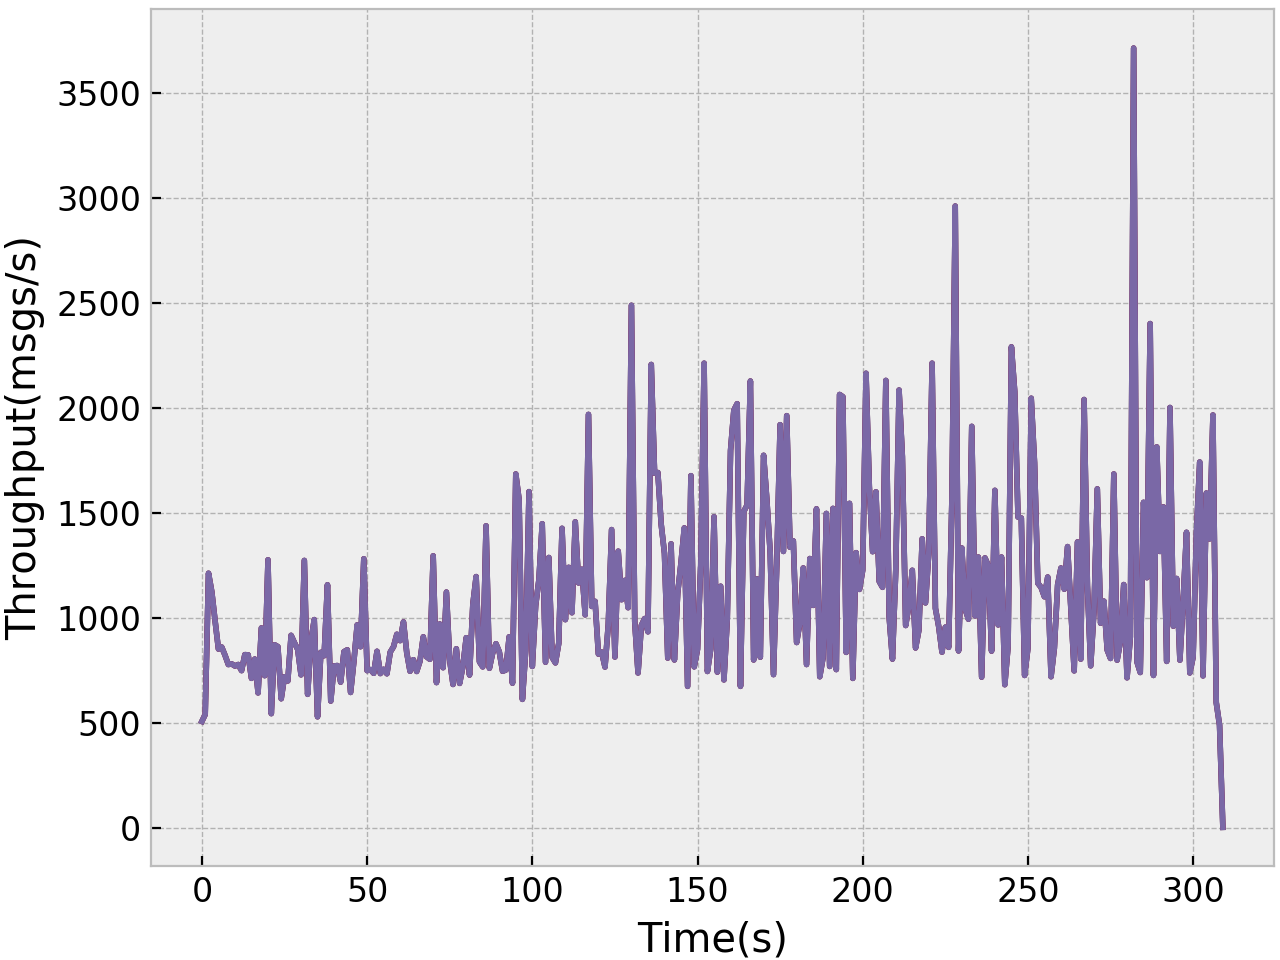
\includegraphics[width=0.49\textwidth,height=\textheight,keepaspectratio]{img/local5_tp.png}
  \caption{ picture that shows client loads }
  \label{fig:local5-performance}
\end{figure}

\begin{figure}[!htb]
  \centering
  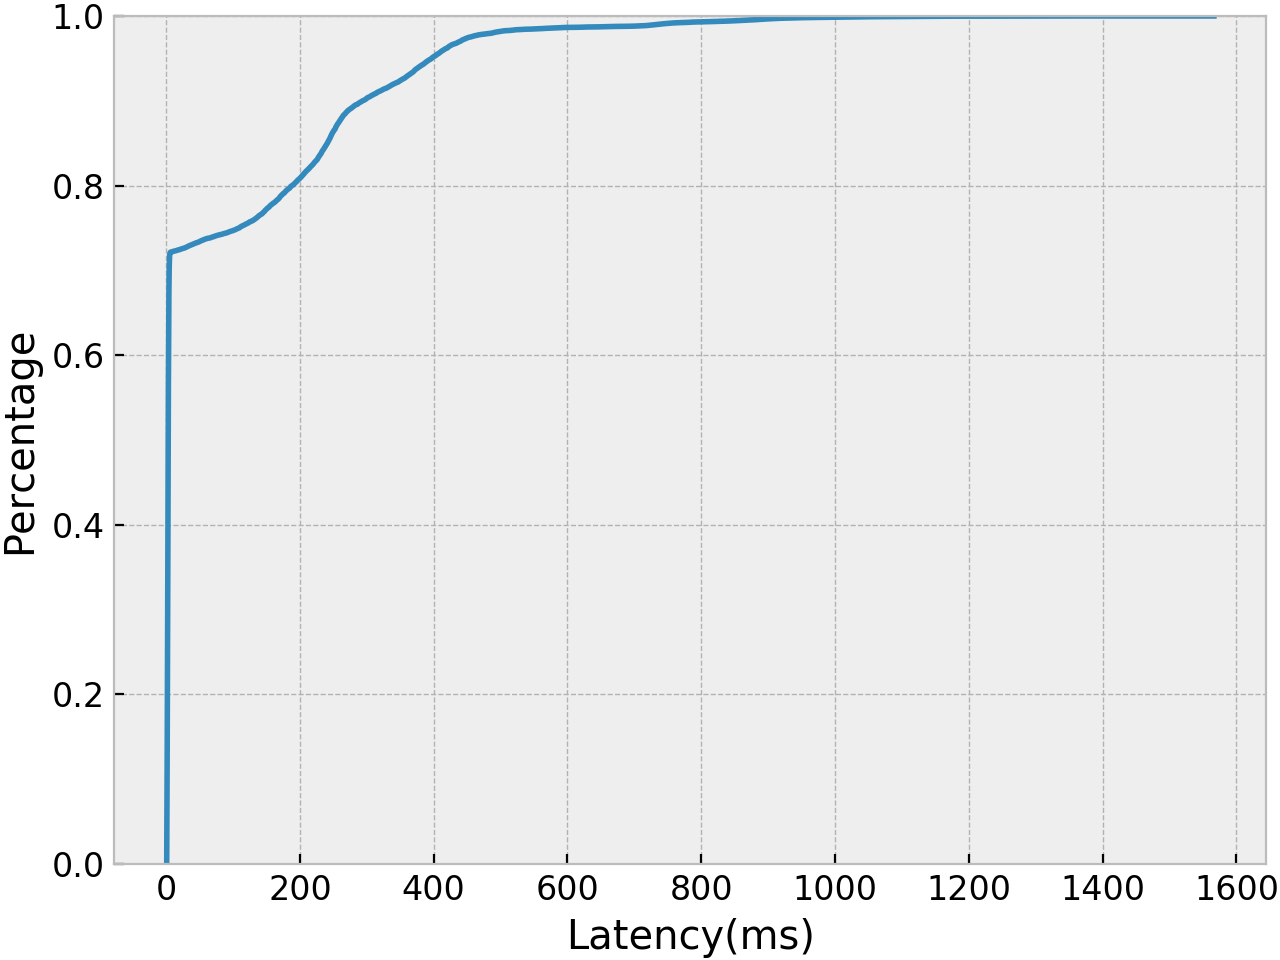
\includegraphics[width=0.49\textwidth,height=\textheight,keepaspectratio]{img/local1_lat.png}
  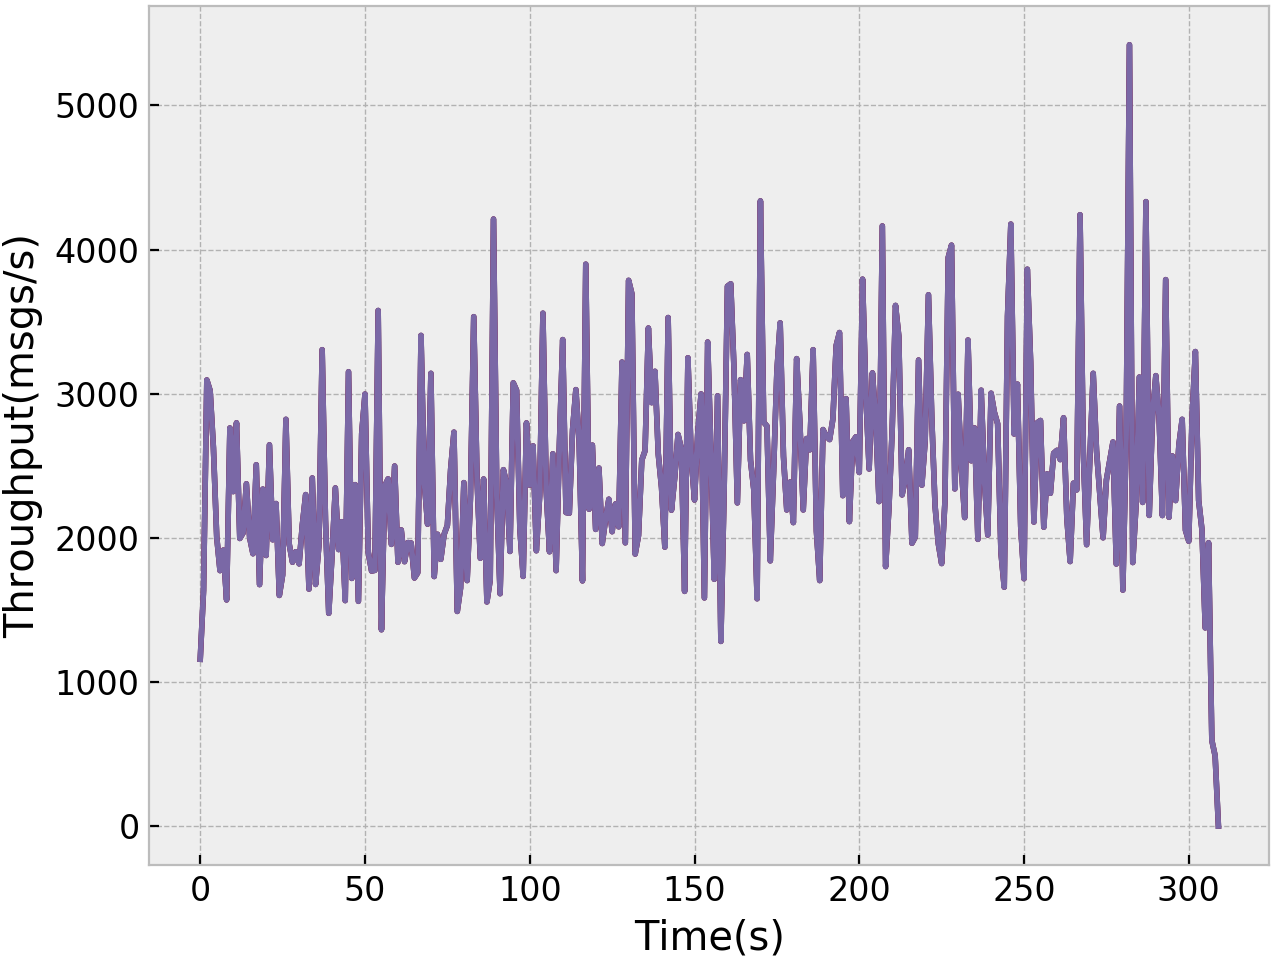
\includegraphics[width=0.49\textwidth,height=\textheight,keepaspectratio]{img/local1_tp.png}
  \caption{ picture that shows client loads }
  \label{fig:local1-performance}
\end{figure}

The plots regarding the tests with 90, 95 and 99 percent reads are pretty much as expected. The average throughput is slightly higher whenever we increase the amount of reads, since reads don't always require all the partitions to synchronize, allowing to perform multiple reads in parallel. The latencies follow a similar pattern, where the more reads we have, the lower the latencies are on average.

The unexpected results are with the test with 50\% reads, which surprisingly has both high throughput and many messages with low latencies. Upon further inspections, we noticed that this was due to the repartitions assigning nodes to different groups. For the nodes handling keys that are evenly shared between groups (for example, in Figure \ref{fig:local-skewed-loads}, we see this around keys 0, 38, 62 and 100) the repartitioning algorithm assigns those nodes to only one group, while in the tests with higher reads percentages these nodes are assigned all the groups (1, 2, 3). From the point of view of the algorithm, this makes sense: since in the first test we have 50\% reads, it is better to assign the nodes to only one group, to favor the write operations. Instead, in the tests with many reads, having these nodes assigned to multiple groups increases the performance with reads. This is why in the first test we have so many messages with close to zero latency.


\begin{table}[!htb]
  \centering
  \begin{tabular}{l l l l l l l l}
    \hline
    & \textbf{Mean} & \textbf{5\%} & \textbf{25\%} & \textbf{50\%} & \textbf{75\%} & \textbf{95\%}& \textbf{99\%} \\
    \hline
    \textbf{50\% reads} & 150 & 37 & 540 & 540 & 540 & 540 & 540 \\
    \textbf{90\% reads} & 150 & 37 & 540 & 540 & 540 & 540 & 540 \\
    \textbf{95\% reads} & 150 & 37 & 540 & 540 & 540 & 540 & 540 \\
    \textbf{99\% reads} & 150 & 37 & 540 & 540 & 540 & 540 & 540 \\
    \hline
  \end{tabular}
  \caption{asd}\label{tab:local-latencies-table}
\end{table}


\subsection{global-skewed}\label{sec:global-skewed}
Another possible view on client behavior in geographically distributed environments is the opposite of the previous one. Instead of having ``local loads'' that depend on the geographic locations of the clients, we could instead have one global load that is shared among all the clients. Examples of objects that could lead to this behavior are viral news that could interest the whole world, or famous people that have fans from all across the globe.

For the test we have similar loads as before, but this time they are not shifted, meaning that all clients access the same keys with the same distribution. This can be seen in Figure \ref{fig:global-skewed-loads}.

\begin{figure}[!htb]
  \centering
  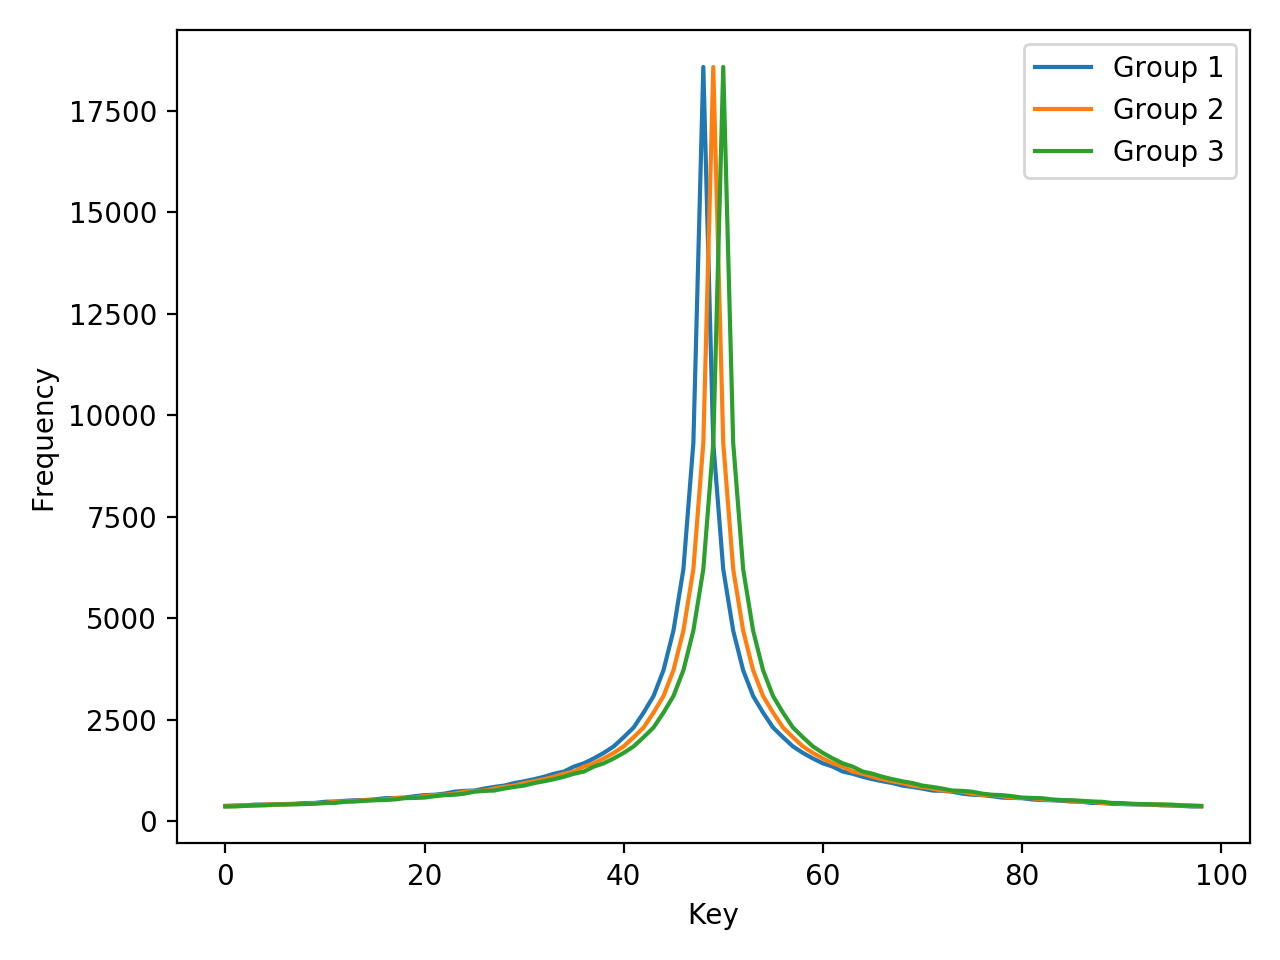
\includegraphics[width=\textwidth,height=\textheight,keepaspectratio]{img/clients_loads_global.png}
  \caption{ global-skewed-loads }
  \label{fig:global-skewed-loads}
\end{figure}

The results we expect to see is that the nodes will more or less have similar partitions, since the accesses that they receive from the clients are the similar.

\begin{figure}[!htb]
  \centering
  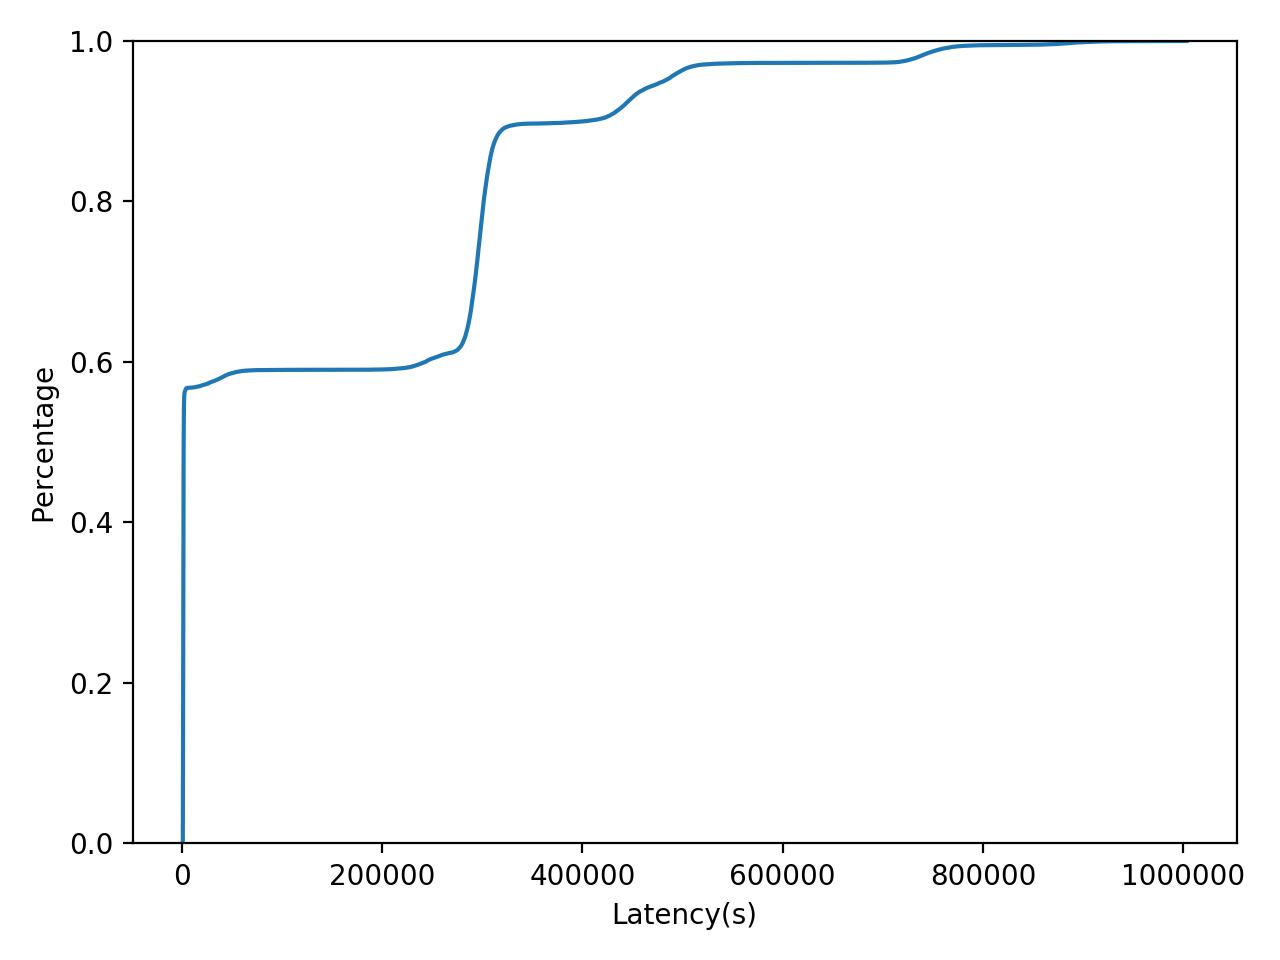
\includegraphics[width=0.49\textwidth,height=\textheight,keepaspectratio]{img/global50_lat.png}
  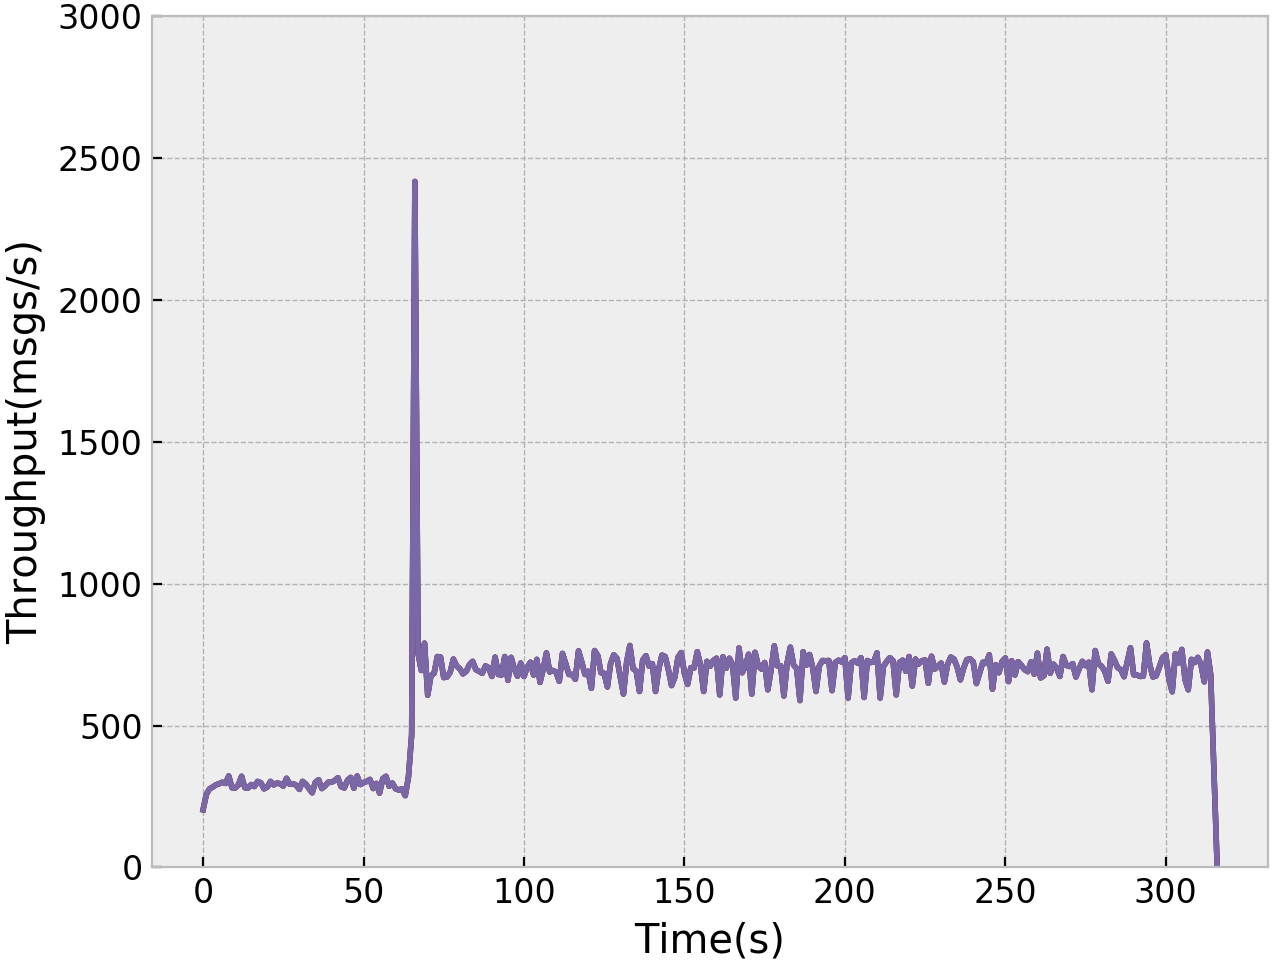
\includegraphics[width=0.49\textwidth,height=\textheight,keepaspectratio]{img/global50_tp.png}
  \caption{ 50\% global }
  \label{fig:global50-performance}
\end{figure}

\begin{figure}[!htb]
  \centering
  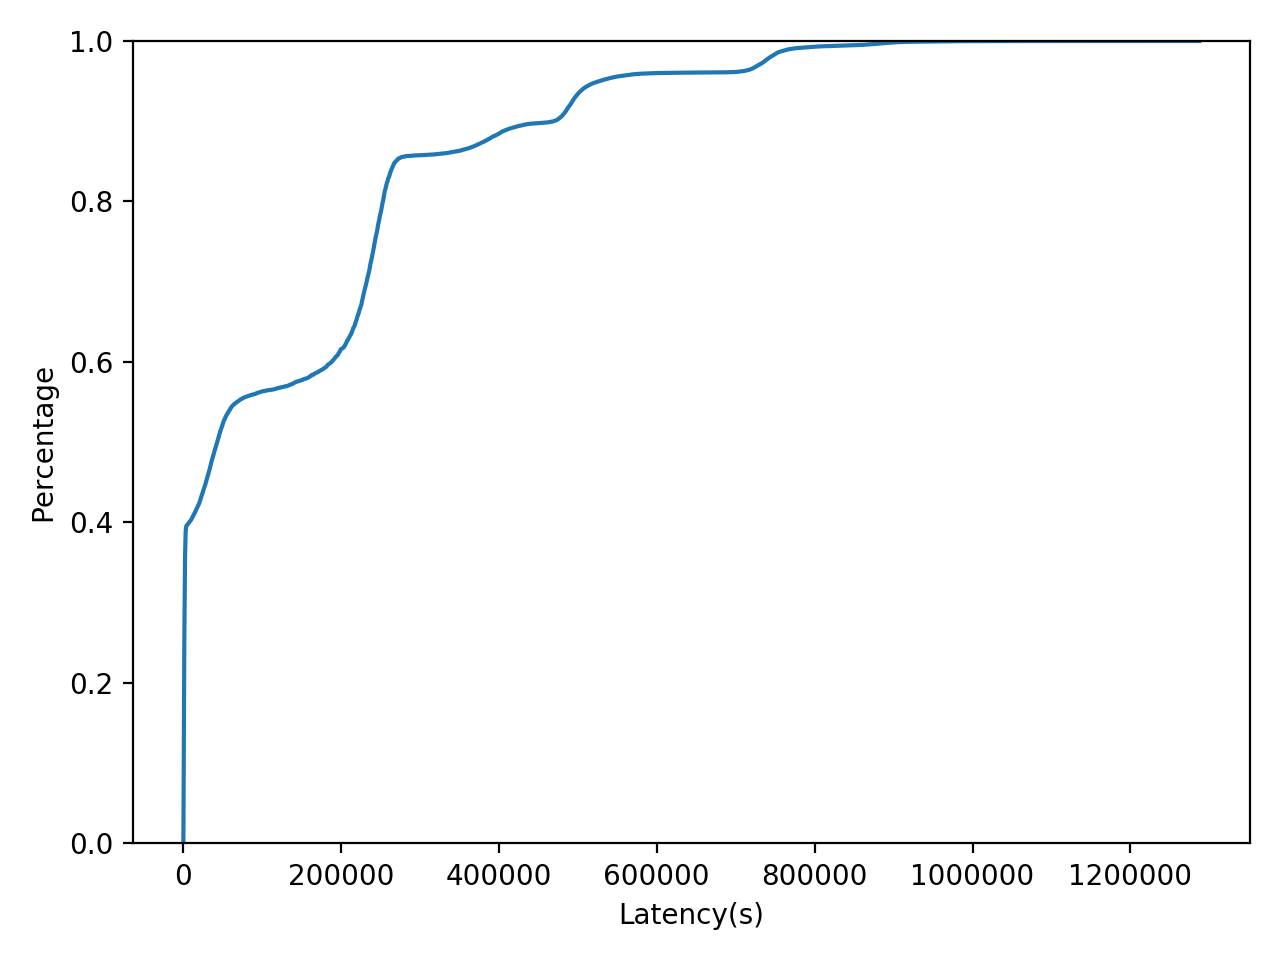
\includegraphics[width=0.49\textwidth,height=\textheight,keepaspectratio]{img/global10_lat.png}
  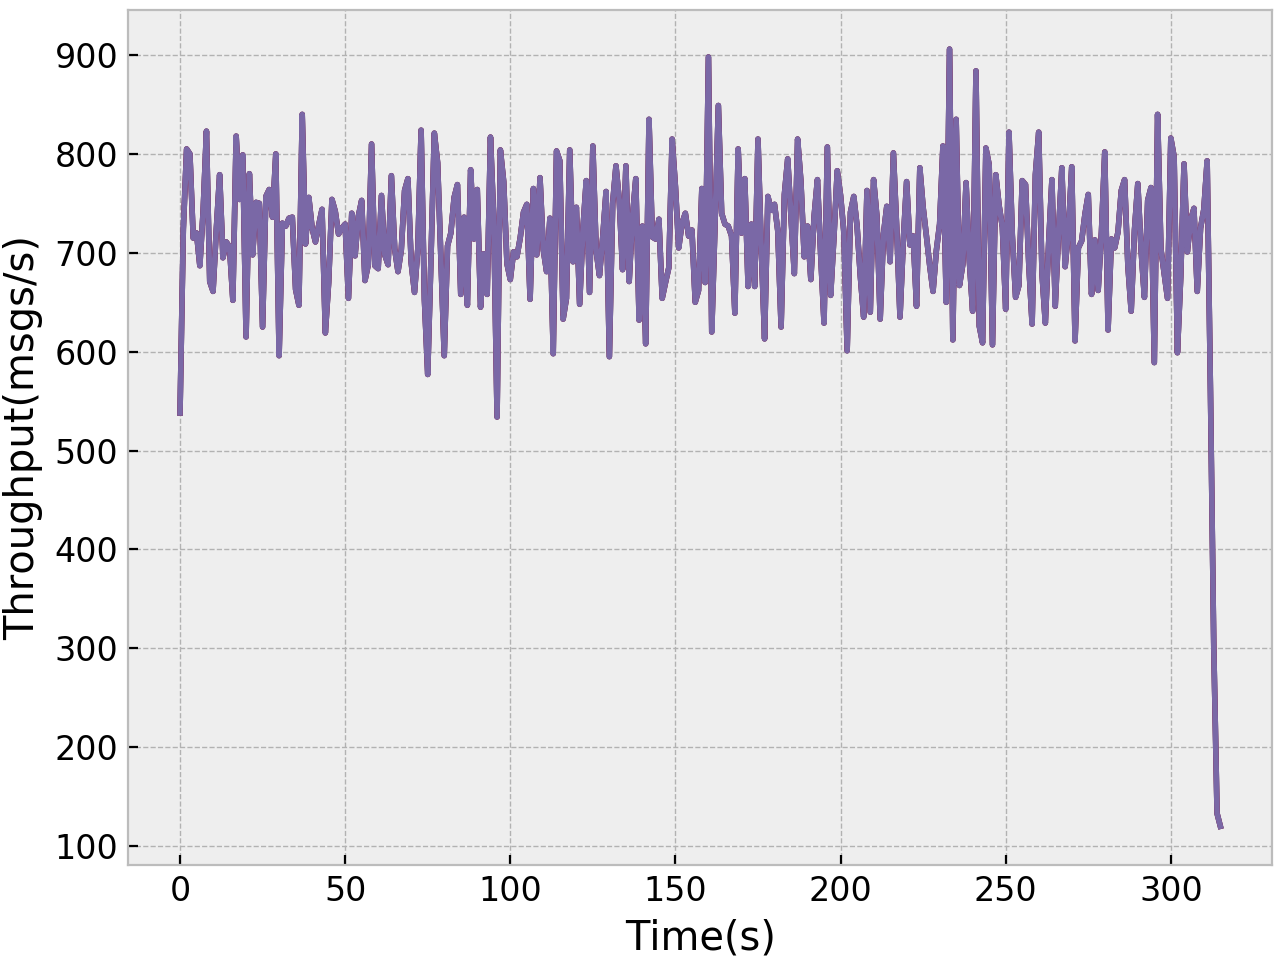
\includegraphics[width=0.49\textwidth,height=\textheight,keepaspectratio]{img/global10_tp.png}
  \caption{ 90\% global }
  \label{fig:global10-performance}
\end{figure}

\begin{figure}[!htb]
  \centering
  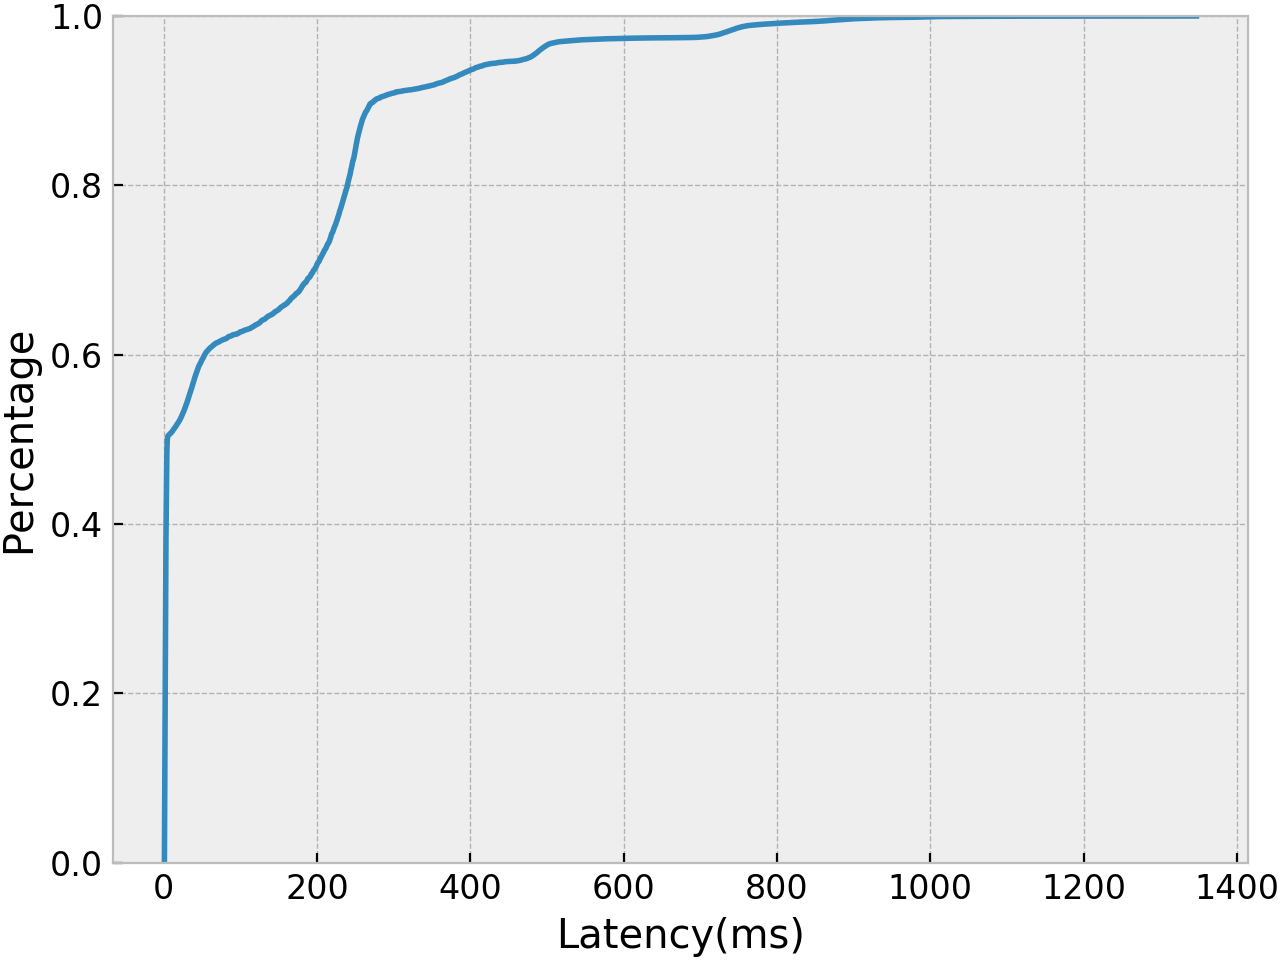
\includegraphics[width=0.49\textwidth,height=\textheight,keepaspectratio]{img/global5_lat.png}
  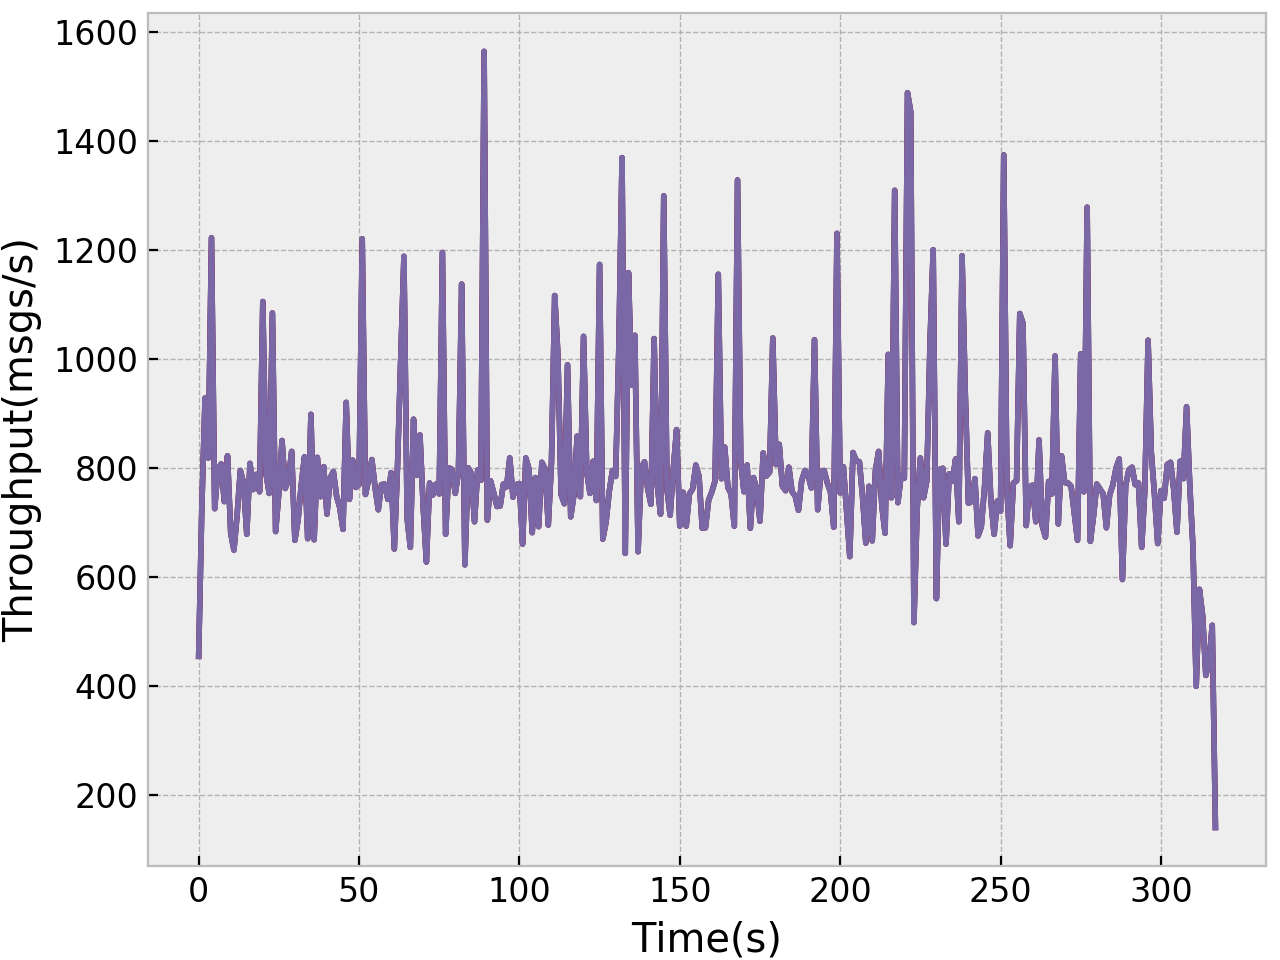
\includegraphics[width=0.49\textwidth,height=\textheight,keepaspectratio]{img/global5_tp.png}
  \caption{ 95\% global }
  \label{fig:global5-performance}
\end{figure}

\begin{figure}[!htb]
  \centering
  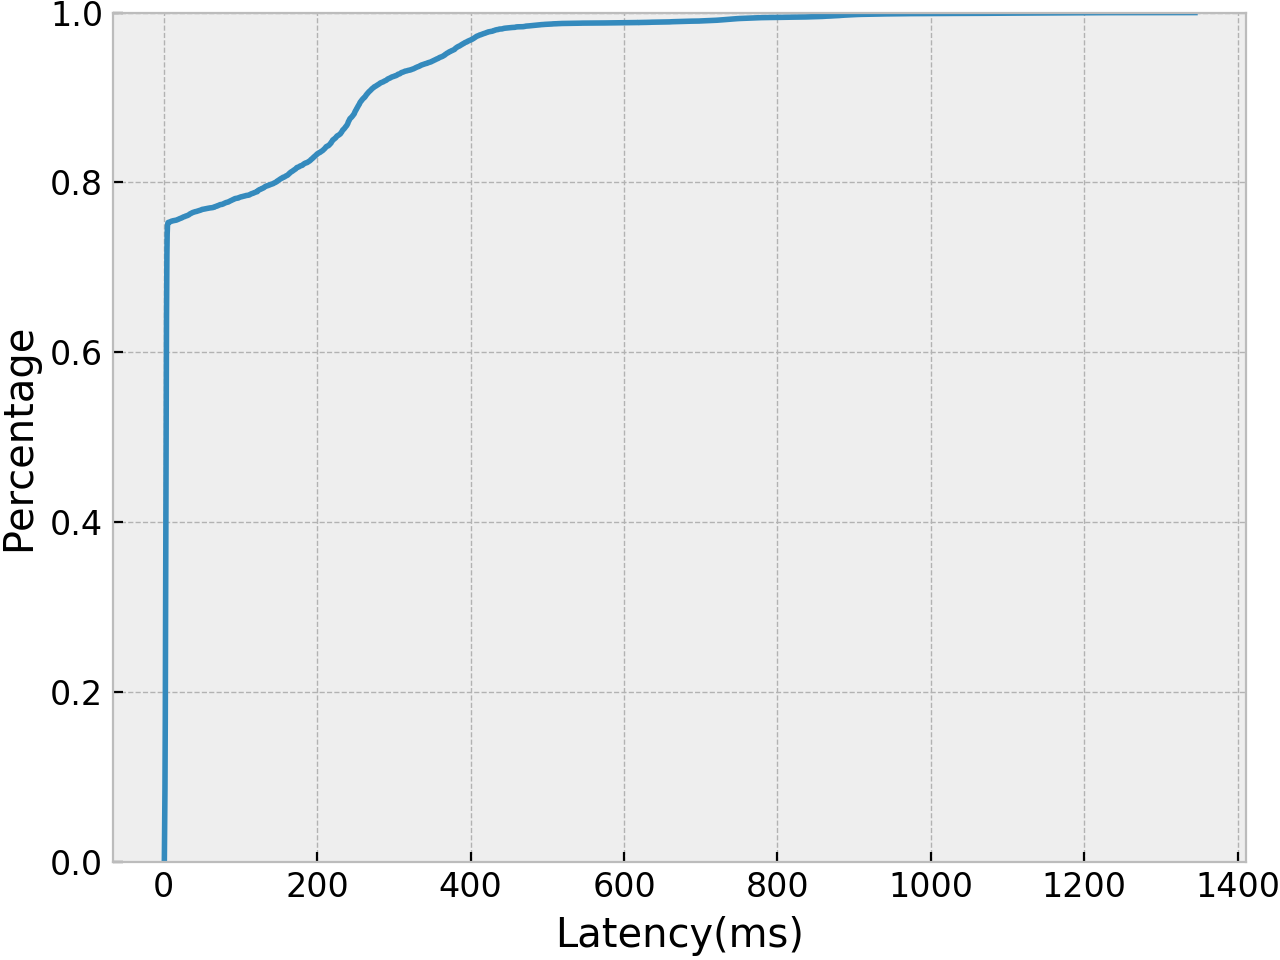
\includegraphics[width=0.49\textwidth,height=\textheight,keepaspectratio]{img/global1_lat.png}
  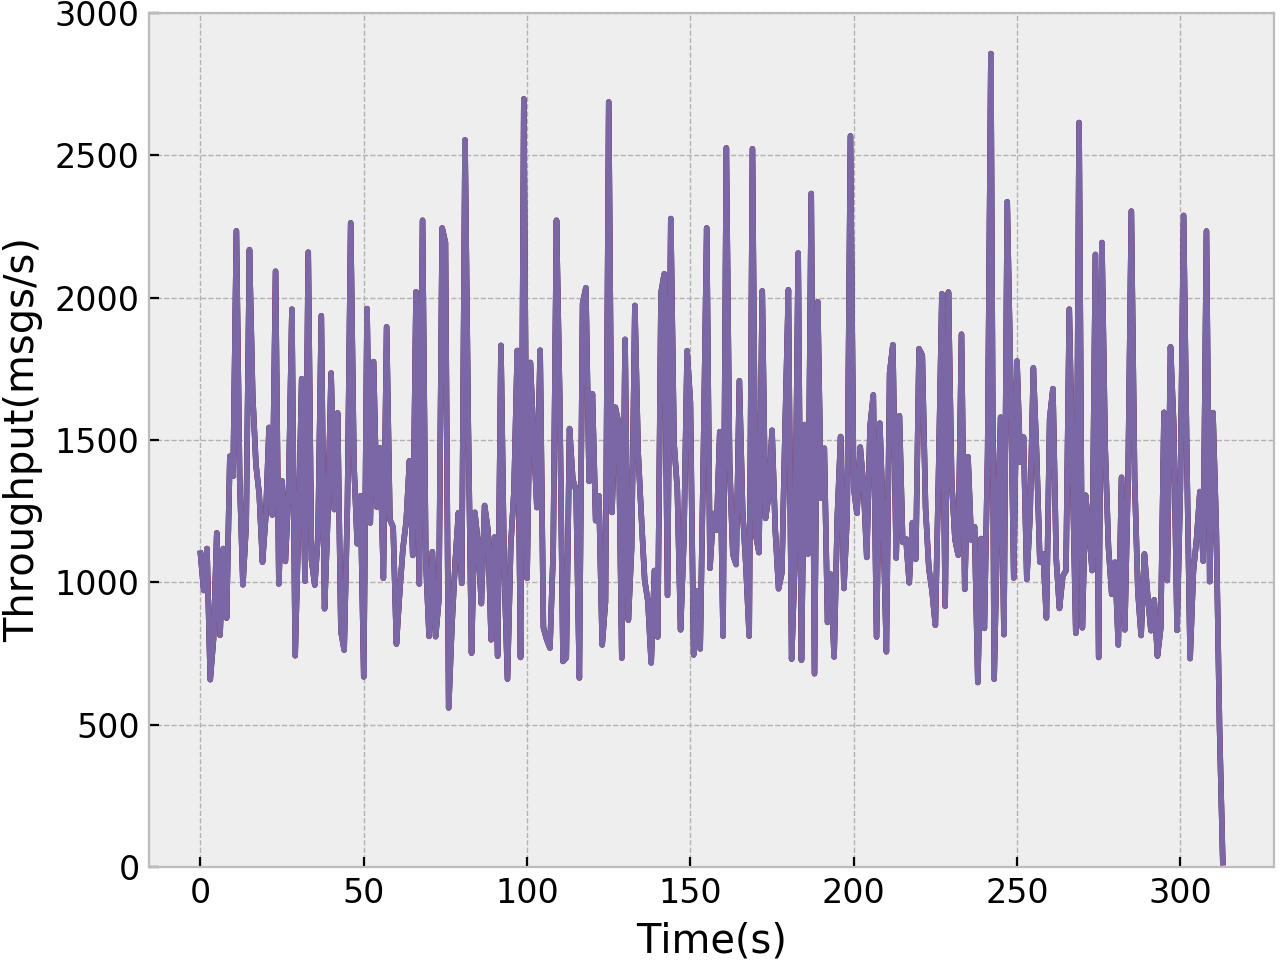
\includegraphics[width=0.49\textwidth,height=\textheight,keepaspectratio]{img/global1_tp.png}
  \caption{ 99\% global }
  \label{fig:global1-performance}
\end{figure}

The results of the global tests are as expected. The throughput are higher in the tests with more read operations. we don't see any improvements in throughput during the tests, because the nodes are by default assigned to all groups, and the loads of the clients are almost identical, which means that there is no real way to improve the partitioning. The latencies are on average worse than the tests with local skews, again as expected, since in those tests we were able to perform a partitioning that takes advantage of the locality.

Looking at the latencies there is an interesting stair-like shape, that gets less and less noticeable when increasing the reads. Those could be the plateaus given by the operations that require multiple groups to deliver the messages.



\begin{table}[!htb]
  \centering
  \begin{tabular}{l l l l l l l l}
    \hline
    & \textbf{Mean} & \textbf{5\%} & \textbf{25\%} & \textbf{50\%} & \textbf{75\%} & \textbf{95\%}& \textbf{99\%} \\
    \hline
    \textbf{50\% reads} & 150 & 37 & 540 & 540 & 540 & 540 & 540 \\
    \textbf{90\% reads} & 150 & 37 & 540 & 540 & 540 & 540 & 540 \\
    \textbf{95\% reads} & 150 & 37 & 540 & 540 & 540 & 540 & 540 \\
    \textbf{99\% reads} & 150 & 37 & 540 & 540 & 540 & 540 & 540 \\
    \hline
  \end{tabular}
  \caption{asd}\label{tab:global-latencies-table}
\end{table}

\subsection{constant}\label{sec:constant}
A third possible load would be a test with a flat distribution, achievable with a skew of $alpha = 0$. This test would be a worst case scenario, since there are no different loads from the clients that can be exploited by the system to better distribute the objects. For this case we don't expect a good performance, as probably most nodes will be assigned to the same partitions.

\begin{figure}[!htb]
  \centering
  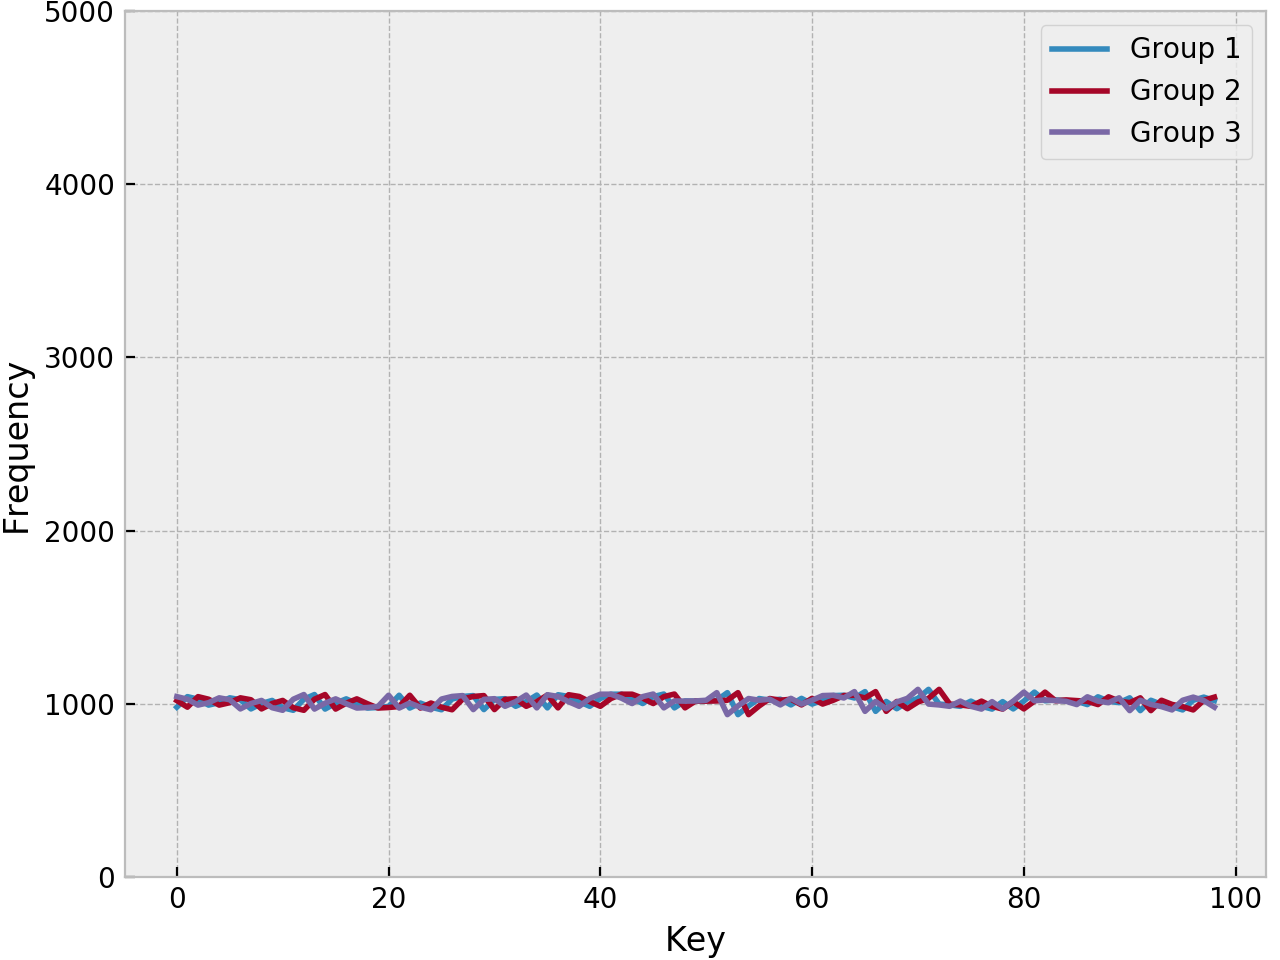
\includegraphics[width=\textwidth,height=\textheight,keepaspectratio]{img/clients_loads_constant.png}
  \caption{ constant-skewed-loads }
  \label{fig:constant-skewed-loads}
\end{figure}

\begin{figure}[!htb]
  \centering
  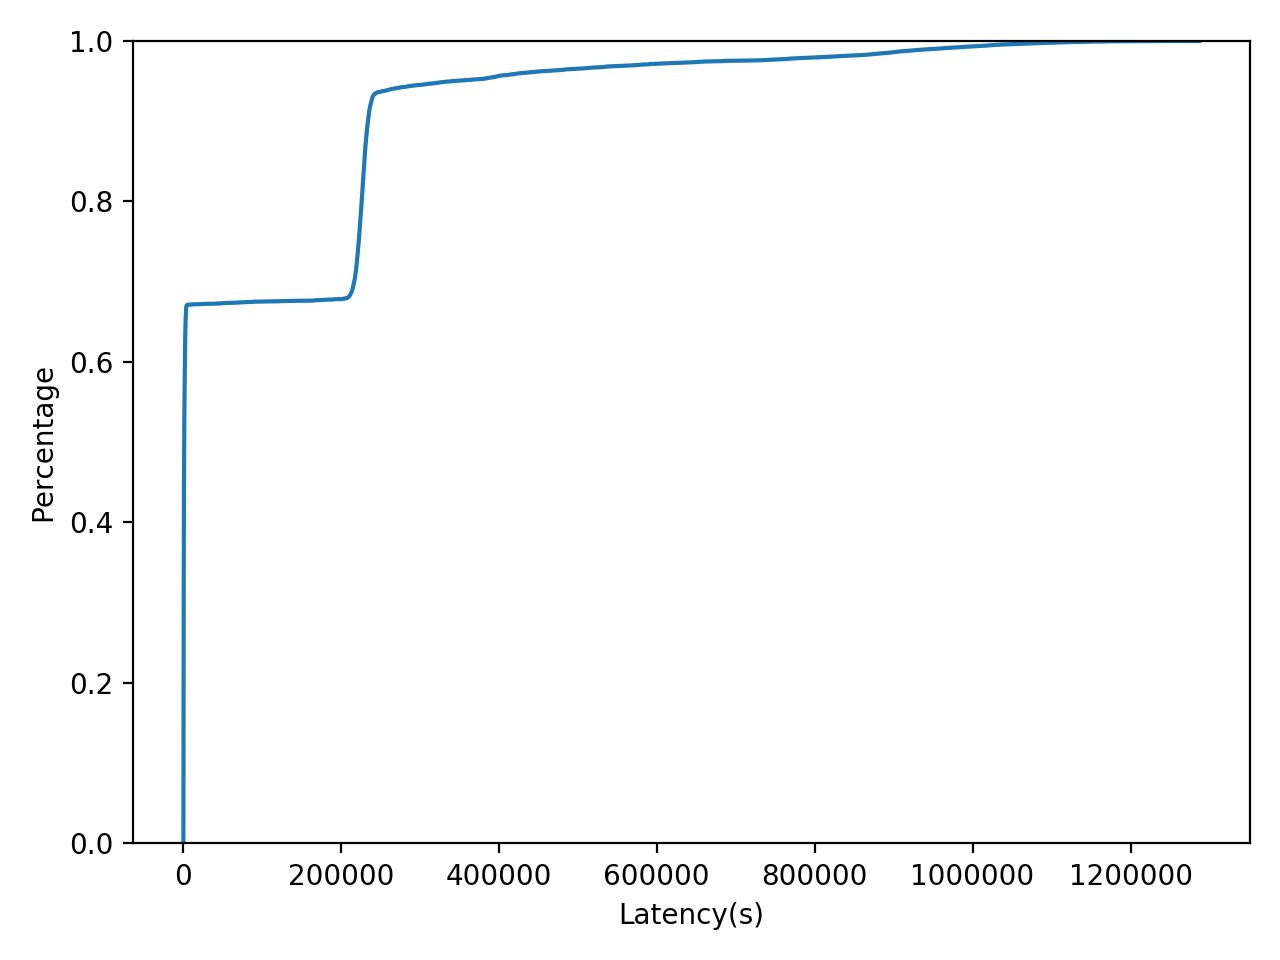
\includegraphics[width=0.49\textwidth,height=\textheight,keepaspectratio]{img/constant50_lat.png}
  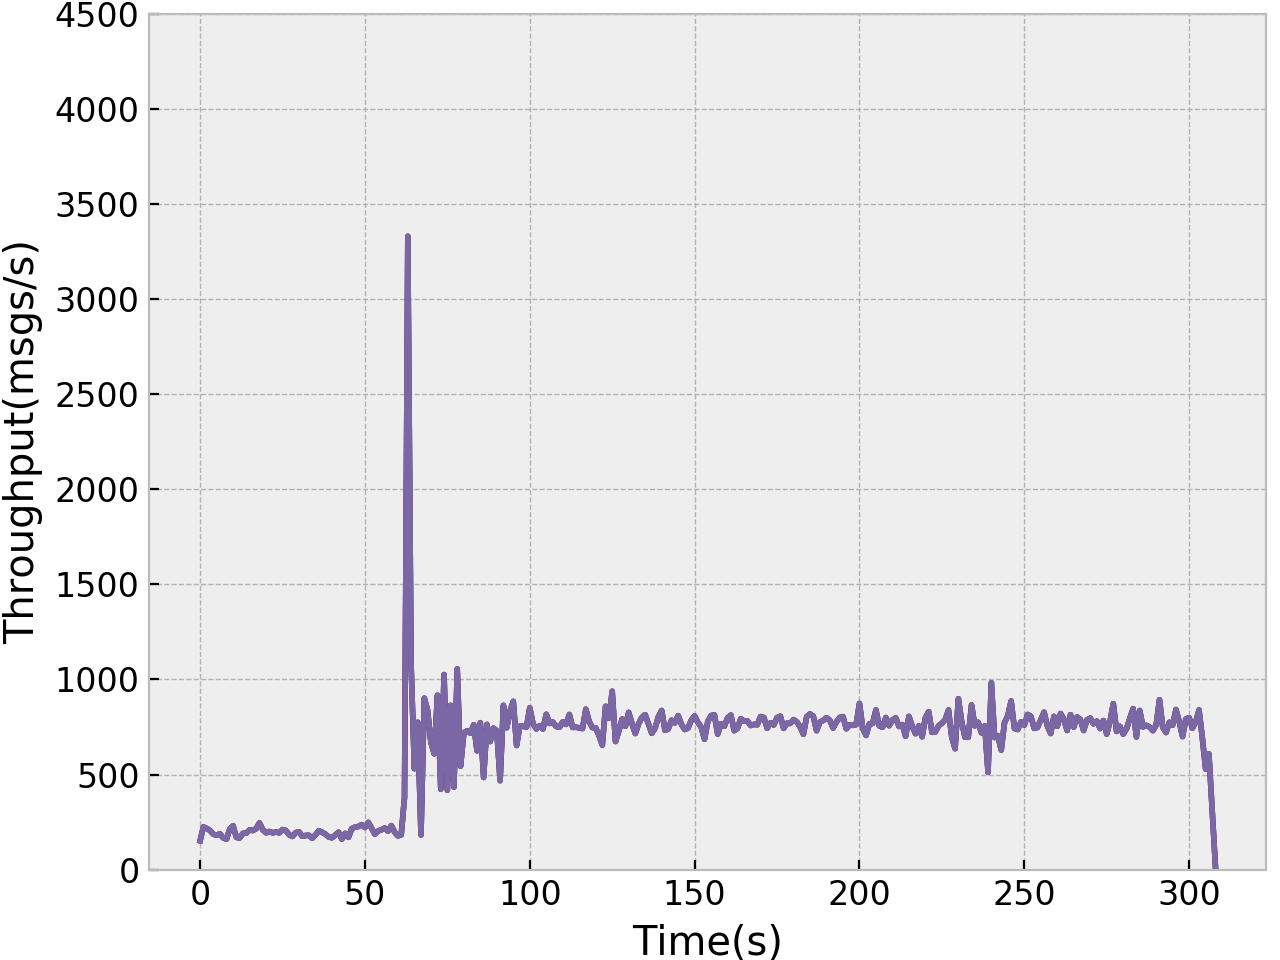
\includegraphics[width=0.49\textwidth,height=\textheight,keepaspectratio]{img/constant50_tp.png}
  \caption{ picture that shows client loads }
  \label{fig:constant50-performance}
\end{figure}

\begin{figure}[!htb]
  \centering
  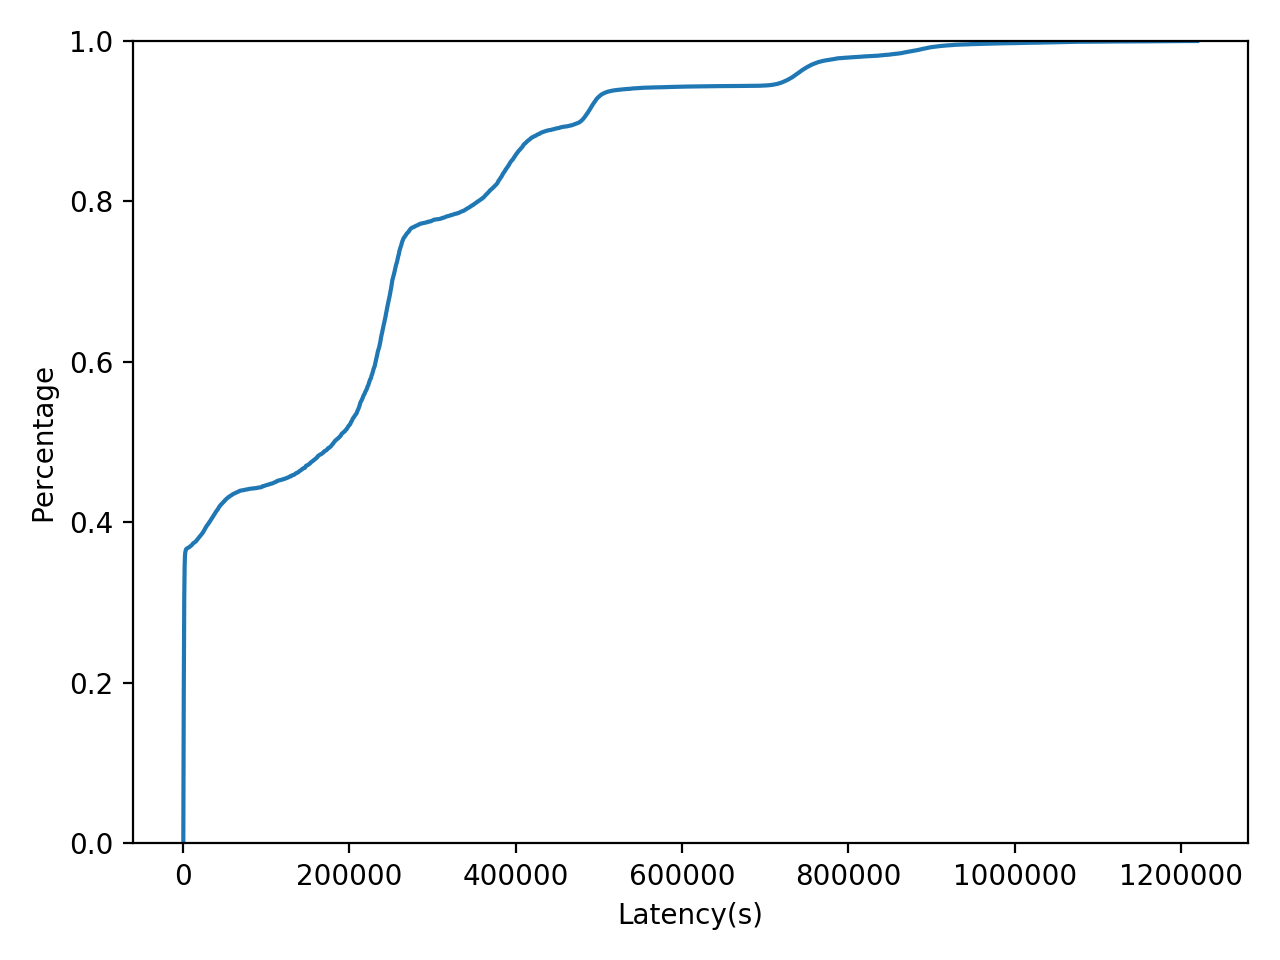
\includegraphics[width=0.49\textwidth,height=\textheight,keepaspectratio]{img/constant10_lat.png}
  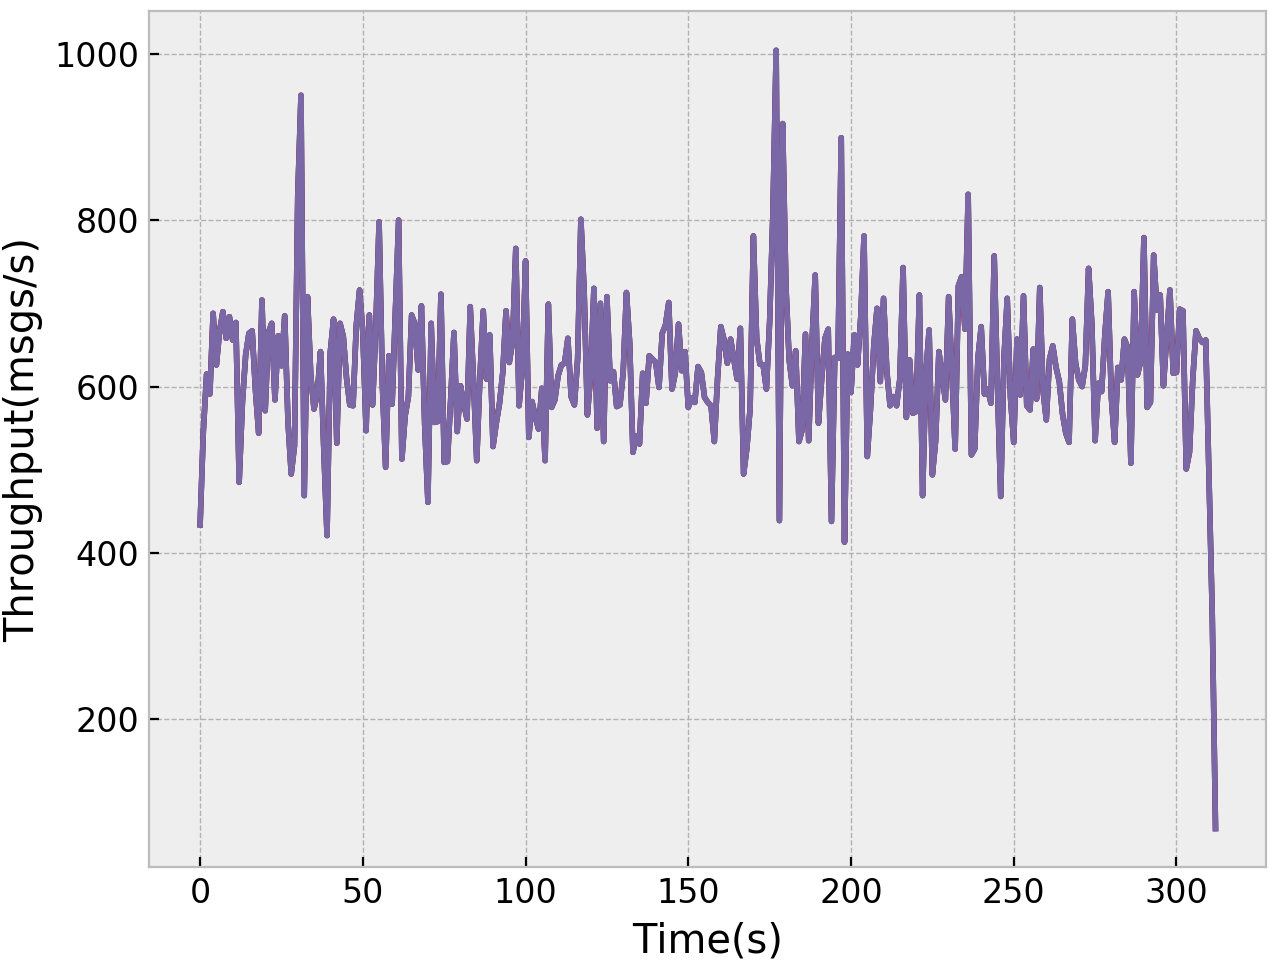
\includegraphics[width=0.49\textwidth,height=\textheight,keepaspectratio]{img/constant10_tp.png}
  \caption{ picture that shows client loads }
  \label{fig:constant10-performance}
\end{figure}

\begin{figure}[!htb]
  \centering
  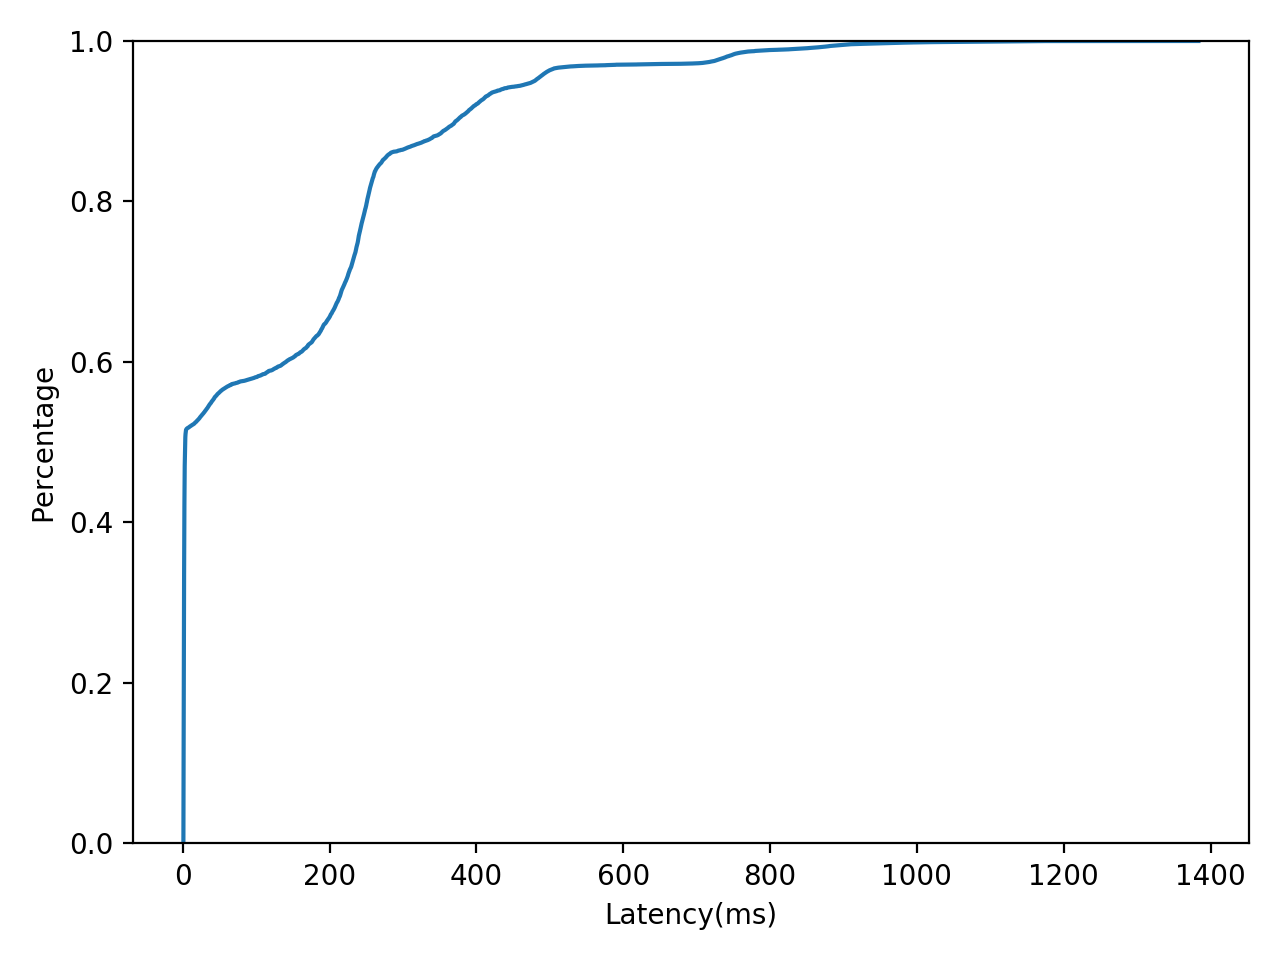
\includegraphics[width=0.49\textwidth,height=\textheight,keepaspectratio]{img/constant5_lat.png}
  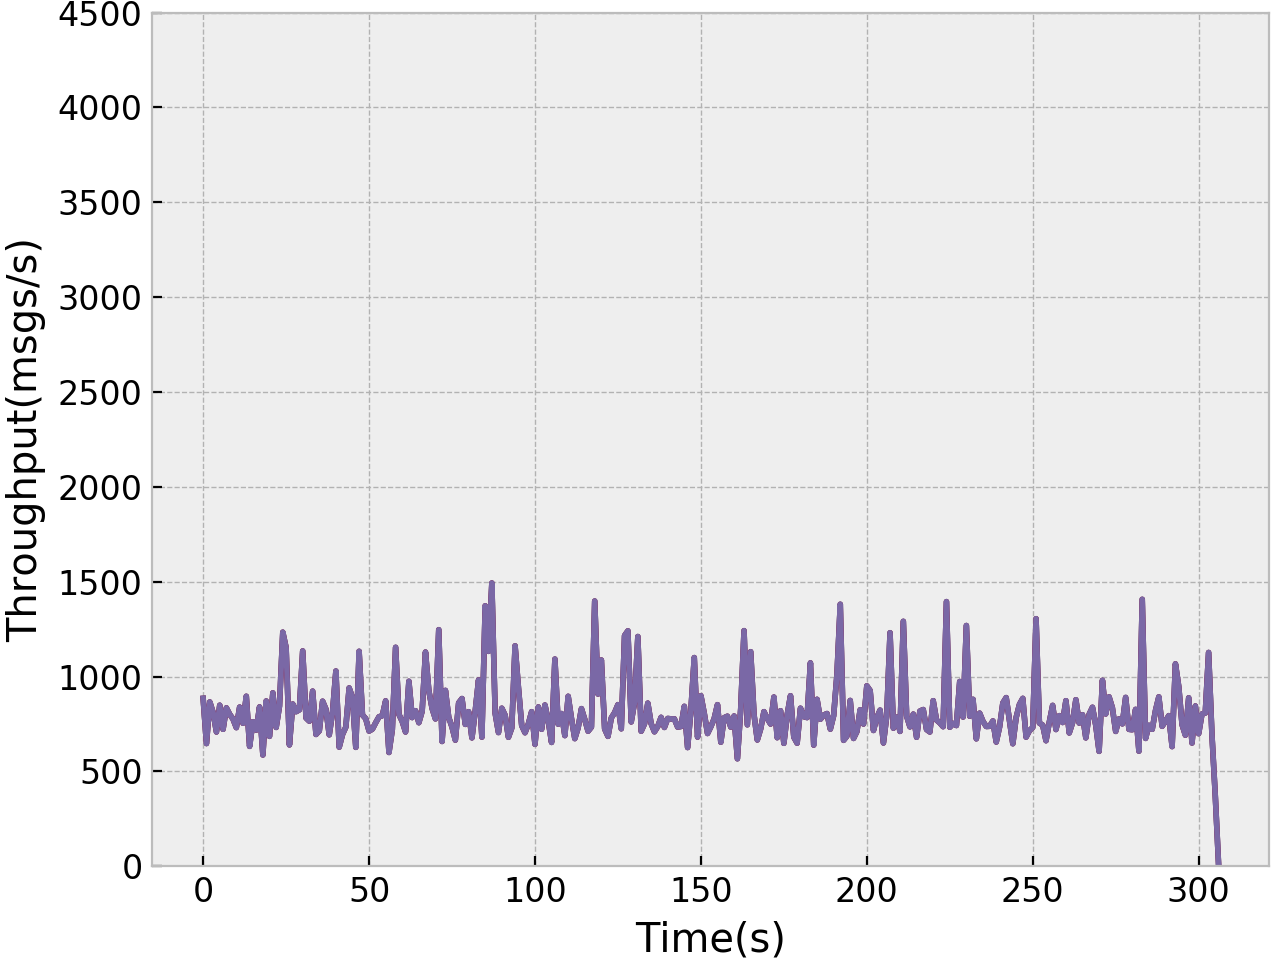
\includegraphics[width=0.49\textwidth,height=\textheight,keepaspectratio]{img/constant5_tp.png}
  \caption{ picture that shows client loads }
  \label{fig:constant5-performance}
\end{figure}

\begin{figure}[!htb]
  \centering
  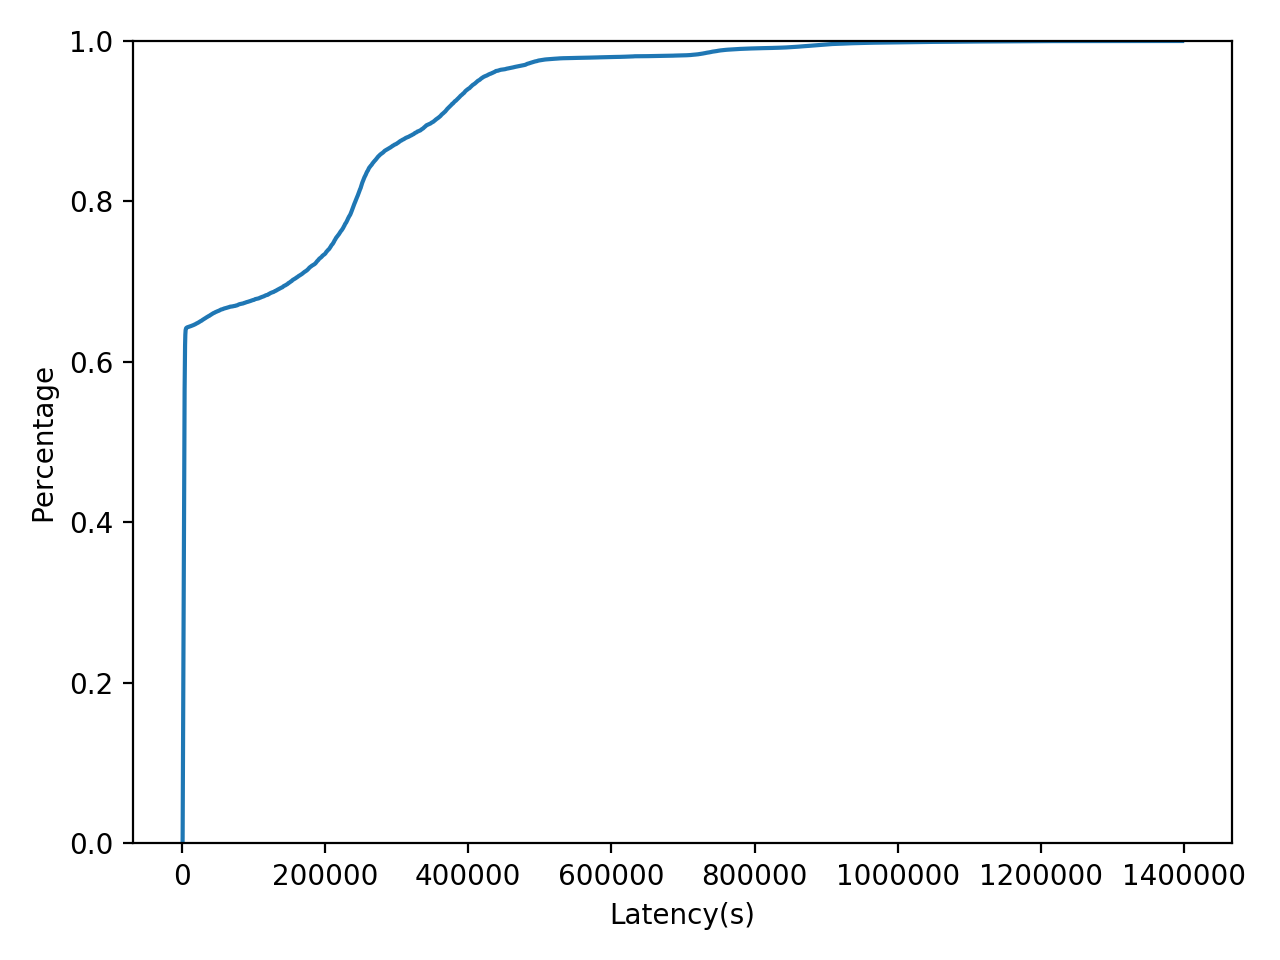
\includegraphics[width=0.49\textwidth,height=\textheight,keepaspectratio]{img/constant1_lat.png}
  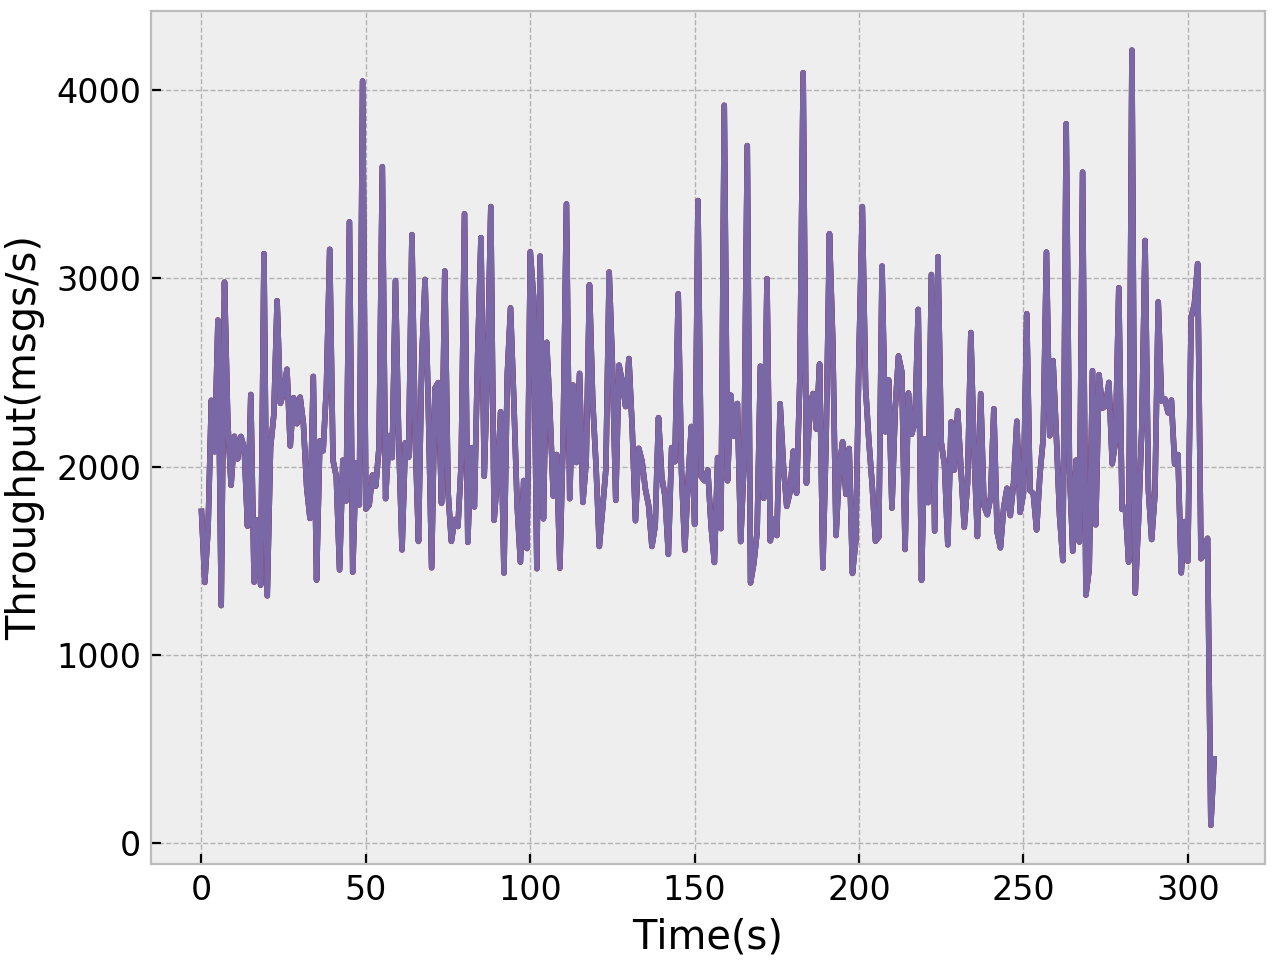
\includegraphics[width=0.49\textwidth,height=\textheight,keepaspectratio]{img/constant1_tp.png}
  \caption{ picture that shows client loads }
  \label{fig:constant1-performance}
\end{figure}

The results are similar to the global-skewed, since in this case the clients have similar behaviors as well. The observations made for the global tests apply for the constant tests as well. Interestingly, in the 50\% read test, the plateaus in the latencies are even more noticeable, perhaps because there's less variation in the combinations of groups destinations.

\begin{table}[!htb]
  \centering
  \begin{tabular}{l l l l l l l l}
    \hline
    & \textbf{Mean} & \textbf{5\%} & \textbf{25\%} & \textbf{50\%} & \textbf{75\%} & \textbf{95\%}& \textbf{99\%} \\
    \hline
    \textbf{50\% reads} & 150 & 37 & 540 & 540 & 540 & 540 & 540 \\
    \textbf{90\% reads} & 150 & 37 & 540 & 540 & 540 & 540 & 540 \\
    \textbf{95\% reads} & 150 & 37 & 540 & 540 & 540 & 540 & 540 \\
    \textbf{99\% reads} & 150 & 37 & 540 & 540 & 540 & 540 & 540 \\
    \hline
  \end{tabular}
  \caption{asd}\label{tab:constant-latencies-table}
\end{table}

\subsection{variable}\label{sec:variable}
This last test is slightly different, since this time we want to test if, and how quickly, the system adapts to a change in workloads. We will initially start with a local-skewed workload like in the first case, and after some time we will shift the clients once more, effectively changing the interest in the objects for all clients. What we expect to see is that after the workload change the performance will drop, and after some repartitions the system will slowly move onto the new partitioning that increases the performance with the new workload. The change in workload is shown in Figure \ref{fig:variable-loads}.

The speed at which the system adapts to the new workload is highly dependant on the $alpha$ variable used when updating the statistics, which defines how quickly the statistics are aging with every repartition. We use an alpha of $0.5$, as from our tests it looked like it was a fine compromise between adaptability and resiliance to unexpected behaviors. A slow adaptation to the new workload would be acceptable, since in our test we are using the most abrupt change possible, which is quite unlikely in a normal execution.

Note that we performed this test only with the 50\% reads load, since what we want to see from this test is not related to the ratio of reads/writes, but just the behavior upon a change of client operations. The test is performed as follows: we start the system with the client loads as in the left image of Figure \ref{fig:variable-loads}. We perform a repartition after 1 minute, and then we repartition every 30 seconds. After 3 minutes and 30 seconds, when we expect the performance to be stable, we stop the clients, and start new ones with distributions as in the right image of Figure \ref{fig:variable-loads}. We then repeat the repartition after 1 minute and then 30 seconds, for at least a couple of minutes to see if the system recovers or not.

\begin{figure}[!htb]
  \centering
  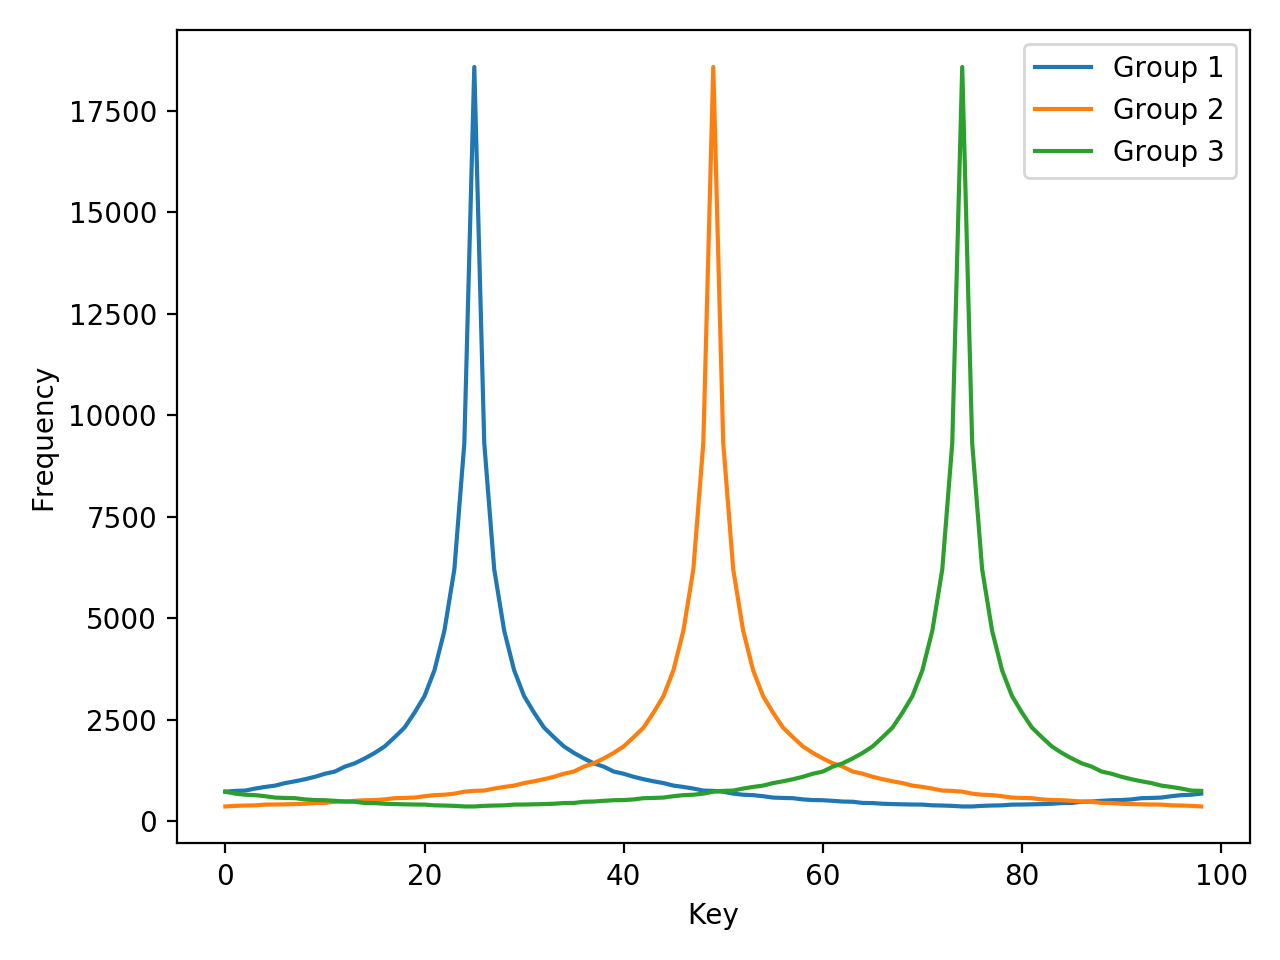
\includegraphics[width=0.49\textwidth,height=\textheight,keepaspectratio]{img/clients_loads.png}
  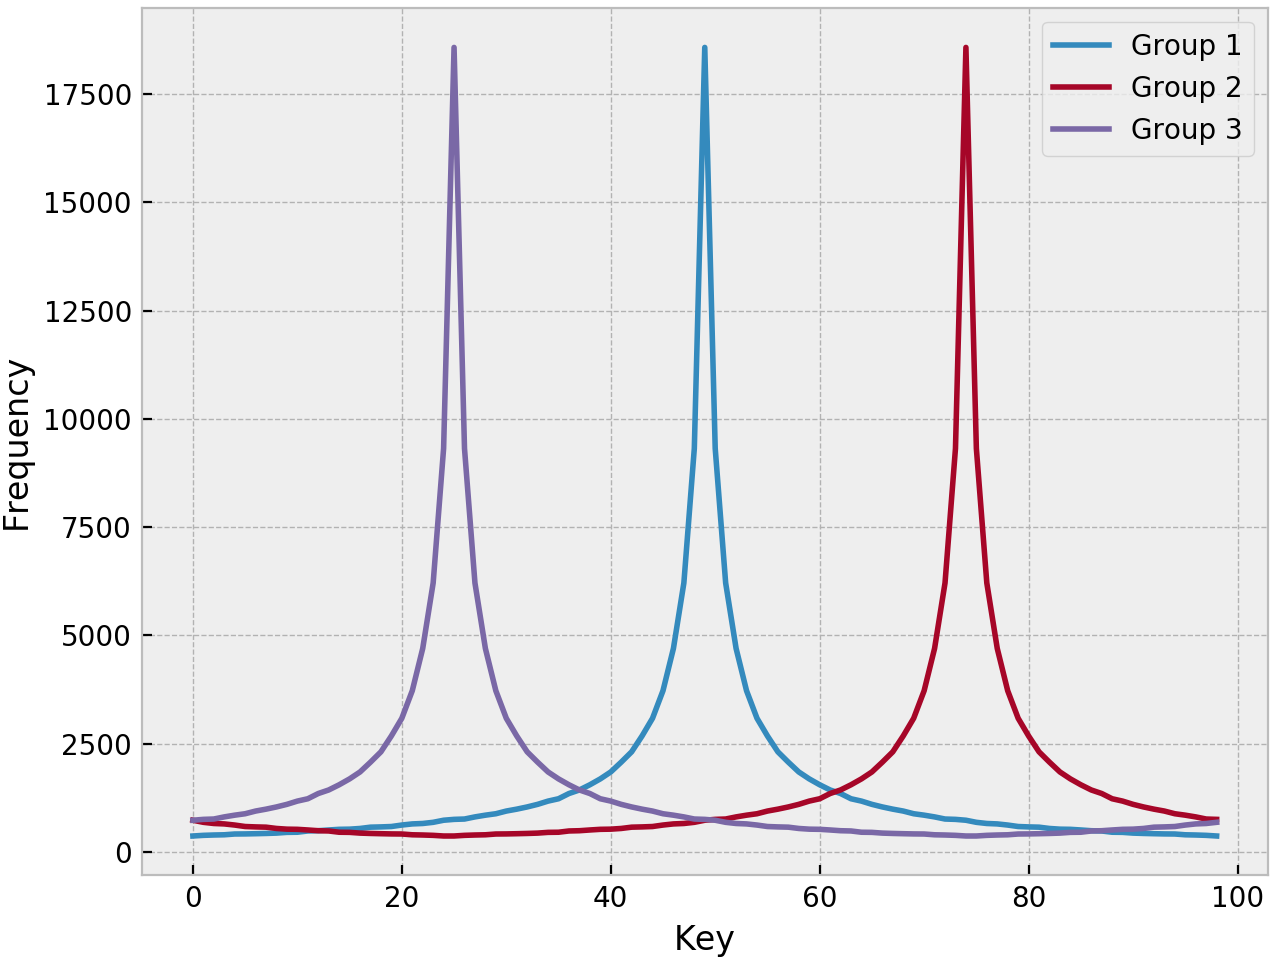
\includegraphics[width=0.49\textwidth,height=\textheight,keepaspectratio]{img/clients_loads_variable.png}
  \caption{ picture that shows client loads }
  \label{fig:variable-loads}
\end{figure}

\begin{figure}[!htb]
  \centering
  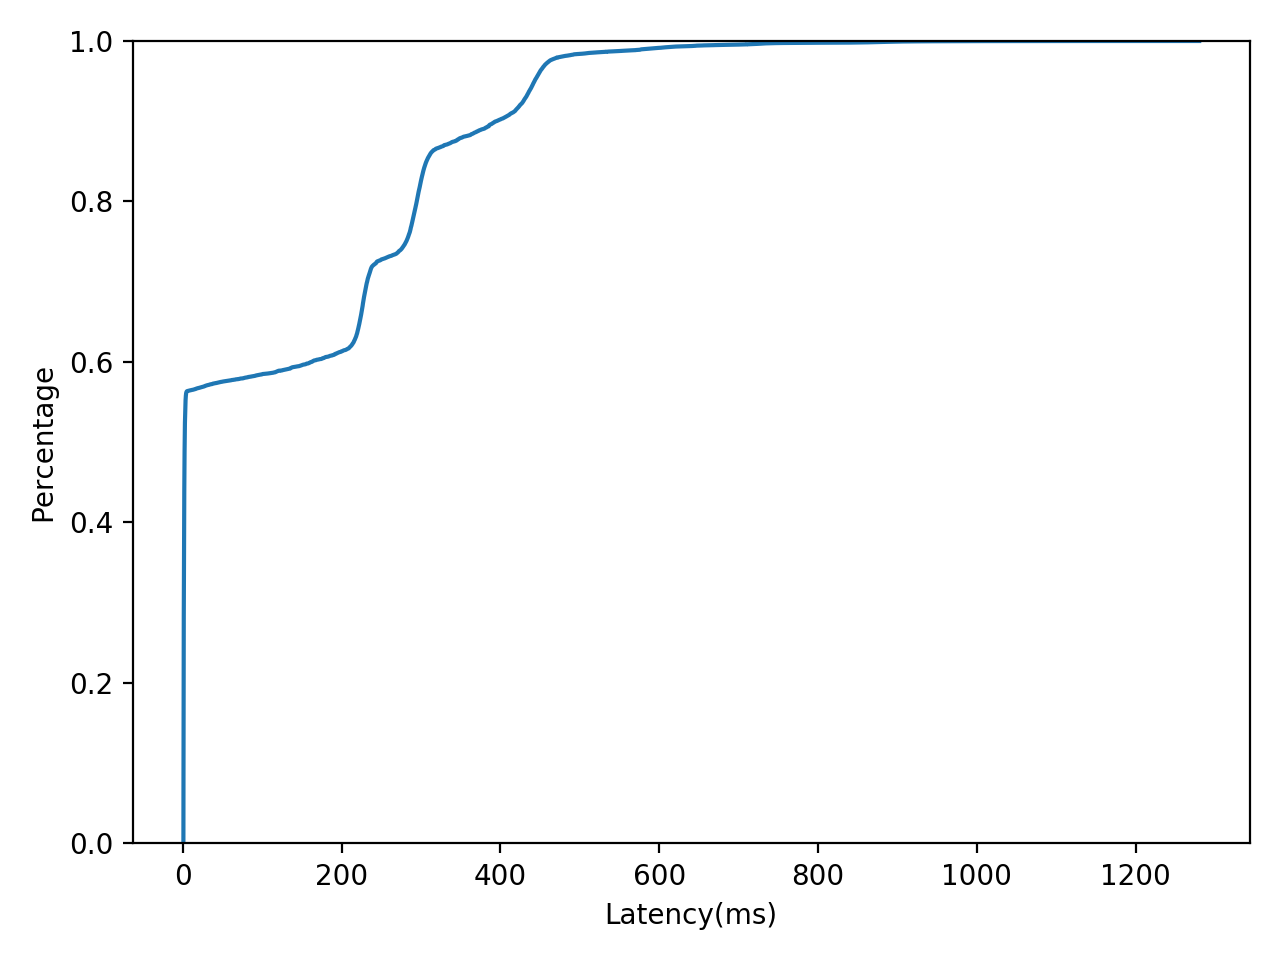
\includegraphics[width=0.49\textwidth,height=\textheight,keepaspectratio]{img/variable50_lat.png}
  \includegraphics[width=0.49\textwidth,height=\textheight,keepaspectratio]{img/variable50_tp.png}
  \caption{ picture that shows client loads }
  \label{fig:variable50-performance}
\end{figure}

The result is quite nice. The latency is nothing particularly different compared to the previous cases, as it shows a similar shape. The throughput instead is a positive result: in the right image of Figure \ref{fig:variable50-performance} we can see the green line that represents the performance with the initial clients, and the red line which represents the performance after we changed the client behavior. The green line behaves as usual, with noticeable increments in performance at the 90 and 120 seconds mark, which correspond to two repartitions. Once we change the clients, the performance drops, since the partitioning is not optimal for the new clients. After the second repartition with the new clients, at 280 seconds, we see that the performance goes back up, meaning that the system adapted to the new clients, and that the repartition correctly re-assigned the nodes based on the recent operations of the new clients.

\clearpage
\section{GeoPaxos Results Evaluation}\label{sec:geopaxos-results-evaluation}
Let us now analyze the results of the tests of the B+ Tree with GeoPaxos, and see if there are some interesting patterns or behaviors that are noteworthy.

\subsubsection{read/write ratios performance}
As expected, in general the tests with more read than writes show better performance. This is the expected behavior, since we don't always need to involve all the replicas that handle an object for a read operation, and furthermore GeoPaxos allows read operations to be performed in different orders in the case where the two operations do not conflict.

\subsubsection{different partitionings}
One interesting exception happened in the local-skewed test, where the different ratio of reads and writes made it so that the nodes where partitioned differently, which ended up increasing the throughput by quite a noticeable margin. This is interesting because we were not expecting this to happen, but on further analyis it made sense that such a case could have happened.

\subsubsection{resiliance}
Another interesting result is that the constant and global-skewed tests have their partitions and throughput almost costant troughout all the tests. what could have happened instead was that because of an uneven period of operations, one region could have monopolized the system, ending up with the repartitioning favoring this one region with an avalanche effect. Fortunately this did not happen, which means that the repartitioning is not too susceptible to such events.

\subsubsection{Plateaus}
Regarding the graphs of the latencies, we have plateaus which are particularly noticeable in the tests with few read operations. These can almost certainly explained by the importance of multi-group operations. In the tests with 50\% writes, we have many occurrences where a message has to be ordered by a set of groups, which on average will have a latency cost that is highly dependant on the geographic location of the groups, and therefore the messages ordered by the same set of groups will have very similar latencies. Therefore, we will have that these operations are grouped together, ending up with the stair-like shape of the latency graphs. 

\subsubsection{variable test}
The variable test case, which was the more peculiar one, showed good results as well. the system adapted quite quickly to the change in clients behaviors, bringing the throughput back to normal levels after a couple of repartitions. This makes us think that the approach is definitely usable in more complicated and variable environments.

\subsubsection{conclusion}
In conclusion, the tests showed positive behaviors, with no particularly surprising results. Obviously the tests were hand-made and highly specific, therefore they can only give an approximate idea of the working of the system; further real world tests would have to be performed, with more complicated and realistic situations. Still, the results do show that the concept idea has some interesting qualities for possible future usages.

% Regarding the graphs of the latencies, we have plateaus which are particularly noticeable in the tests with few read operations. These can almost certainly explained by the importance of multi-group operations. In the tests with 50\% writes, we have many occurrences where a message has to be ordered by a set of groups, which on average will have a latency cost that is highly dependant on the geographic location of the groups, and therefore the messages ordered by the same set of groups will have very similar latencies. Therefore, we will have that these operations are grouped together, ending up with the stair-like shape of the latency graphs. 

% constant before a repartition is faster than local, because the loads are evenly distributed, less change to conflict keys

